\documentclass[oneside]{book}

%TODOTODOTODOTODOTODOTODOTODOTODOTODOTODOTODOTODOTODOTODOTODOTODOTODOTODO
%juiste git commit voorzien!!!

% Load the VUB package.
% This has many options, please read the documentation at
% https://gitlab.com/rubdos/texlive-vub
\usepackage{vub}

%href package to make references clickable.
\usepackage{hyperref}
\hypersetup{
    colorlinks,
    citecolor=black,
    filecolor=black,
    linkcolor=black,
    urlcolor=black
}

%subfigures
\usepackage{caption}
\usepackage{subcaption}
\usepackage{wrapfig}

% Some highly suggested packages, please read their manuals.
\usepackage{cleveref}
\usepackage[natbib,style=apa]{biblatex}
\addbibresource{../bibliography.bib}

%space between paragraph and indent all
\setlength{\parskip}{1em}
\usepackage{indentfirst}

%space between bib entries
\setlength\bibitemsep{2\itemsep}

%images settings
\graphicspath{ {./images/} }
\usepackage{graphicx,caption}
\usepackage{float}
\usepackage{rotating}
\usepackage{tikz}

%fix section numbering for use with parts
\renewcommand*\thepart{\Roman{part}}
\makeatletter
\@addtoreset{section}{part}
\makeatother
\renewcommand*\thesection{\arabic{part}.\arabic{section}}
\renewcommand*\thesubsection{\thesection.\arabic{subsection}}

%START title
% done
\title{Animal classification AI}
\subtitle{Machine Learning}
\author{Lennert Bontinck}
\date{January, 2021}
\promotors{Master Computer Science: AI}
\faculty{Sciences and Bio-Engineering Sciences}
\begin{document}
\frontmatter
\maketitle
%END title


%START abstract
% done
\chapter*{Abstract}

This report documents the development of an \textit{animal classification AI} using a more \textit{old-school approach} of Visual-Bag-of-Words models.
This AI is capable of differentiating 12 different animals.
These models, and thus the AI, are developed in Python-based Jupyter Notebooks accompanied by this document.
This animal classification AI was developed as a fulfilment of the Machine Learning course requirements and was used to compete in the organised Kaggle competition \citep{kaggle_competition}.

Part \ref{part:about_the_code} of this report discusses the accompanied code in general.
Section \ref{section:inc_files} explains which files are the most important. 
Section \ref{section:ideology_dev_code} describes the ideology used to created the code. 
To make testing multiple models easier, \textit{a template} for model exploration was created and is discussed in section \ref{section:typical_model_exploration}.

In part \ref{part:data_analysis}, the \textit{data analysis} part of this project is discussed.
Section \ref{section:DA_data_distribution} talks about the \textit{unbalanced data} distribution.
In the next section, section \ref{section:DA_deeper_look_data}, a deeper look is taken into the data and possible \textit{preprocessing} is discussed.
The last few sections of this part discuss how the \textit{feature extraction} is dealt with and what the numerical representation looks like.

The \textit{linear baseline model} is discussed in part \ref{part:linear_baseline}.
This model is a fine-tuned \textit{Logistic Regression model} from the SciKit Learn library.
This model is often used to compare other models with.
Only models that perform better then this baseline model should be considered.
This part discusses the parameters used and the road to finding those optimal parameters.

Afterwards \textit{Support vector Classifiers} (SVC) are explored.
Part \ref{part:svc} discusses non-linear SVC models with different kernels and finds the \textit{rbf kernel} to be the best from three tested kernels.
Part \ref{part:linear_svc} focuses on linear SVC models in a similar fashion and finds them to perform worse.
An ensemble approach is discussed in part \ref{part:gradien_boost}.
This approach makes use of Gradient Boosting which, while interesting, didn't perform well.

It is chosen to do the model analysis in a separate part, part \ref{part:model_anal}.
Afterwards, part \ref{part:final_model} goes over some other possible optimisations considering what is learned from all experiments thus far.
Some of these are implemented whilst others are just discussed in a theoretical manner.
This results in the final, best performing, model.
Afterwards, in part \ref{part:conclusion}, a short conclusion is given.

It is noted that the page count of this document doesn't represent its actual length due to clear part separation from the used template and large figures.
Content that isn't crucial or is a repetition of supplied information is discarded or given as an appendix.
%END abstract


%TOC
\tableofcontents
\mainmatter

%START about
\part{About the code}
\label{part:about_the_code}

%------------------------------------

\section{Files accompanied by this report}
\label{section:inc_files}
Since this report discusses the development of an AI, \textit{a lot of code} is discussed as well.
This code is not shown inside this document but is available on the GitHub repository \citep{github_project}.
All code is written in Python-based Jupyter Notebooks.

%------------------------------------


\section{Ideology of the developed code}
\label{section:ideology_dev_code}
The Jupyter Notebooks have many inline comments and markdown blocks to make reading the code easier.
If code is extensively discussed in this report, a reference to the corresponding section is made inside the code. 
Some of the gathered results come from time-consuming function calls.
These can take \textit{multiple hours} to complete.
To spare some time, these results are saved in a Pickle file so they can be loaded in without having to do the function call.
The Notebooks are written in a way that makes testing multiple models easy, paying extra attention to reusability. 

%------------------------------------

\section{A typical model exploration}
\label{section:typical_model_exploration}
The testing of a model consists of two main parts.
Firstly the input of the model has to be optimized.
Afterwards, the (hyper)parameters of the model itself can be optimized.
These steps are clearly visible with the discussed models in this report since they follow a form of \emph{template}.
This template makes testing new models rather easy.
After optimizing everything in a standalone fashion, it has to be checked that these newly optimized parameters do not influence previously optimized parameters.
The resulting model should perform better than the linear baseline model in order to be considered.
Whilst many abstractions were made and creating a \emph{one-call pipeline} is possible, it's chosen to not do so.
This is because \textit{human reasoning} can be required in finding truly optimal parameters.
It also makes understanding and discussing the model easier.
After all, the goal of this report is to gather an understanding on how these models work, not solely  to get the best Kaggle score.

%------------------------------------


\section{Technical remarks}
\label{section:technical_remarks}

Most source files, for this report and the created models, are available on GitHub \citep{github_project}. Some files, like the used training images, were not included in this GitHub repository. Details about this can be found on the GitHub page (\texttt{README} file). Rights to this GitHub repository can be asked from the author. This report was created in \LaTeX{} by modifying the VUB themed template from Ruben De Smet (\citeyear{latex_template}).

%START data analysis
\part{Data analysis}
\label{part:data_analysis}

%------------------------------------

\section{About this part}
\label{section:DA_about_part}
Before rigorously testing different models available, it's important to take a look at the data that is supplied. The supplied data consists of 2 main groups of images, labelled training images and unlabeled test images.
As per the requirements of the Kaggle competition, the test images should only be used for evaluating the model on the Kaggle page by submitting a CSV of the prediction results.
Thus the test images can't be used for creating the model in any shape or form.
This means that only the labelled training images can be used to create and validate the model in development.
To avoid altering the model to perform well on the supplied test data and not in general, only the training data will be analysed.
All code used for this part is available under the developed code folder on GitHub, in the Jupyter Notebook \emph{data\_analysis.ipynb}.
This part describes how data can be analysed with the given code.
This code can be easily changed to analyse other variations of the data, e.g. using another descriptor.

%------------------------------------

\section{Data distribution}
\label{section:DA_data_distribution}
The provided labeled training data consists of 12 different classes.
There is a total of 4042 labelled training images supplied, the distribution of which is shown in figure \ref{fig:1-data_analysis-labeled_data_distribution}.
As visible in this figure, the distribution between classes is not balanced.
This has to be taken into account when fitting a model since some models will show unwanted behaviour when fitted with unbalanced data.
Luckily many solutions exist to minify the impact of this unbalance.
This unbalance has to be kept in mind when using a split of the training set as a validation set as well.
This is because such split might lead to a test set where some classes have considerably fewer instances in the test set and thus the performance on those classes has less impact on the total score, which may be unwanted.


\begin{figure}[H]
    \centering
    \fbox{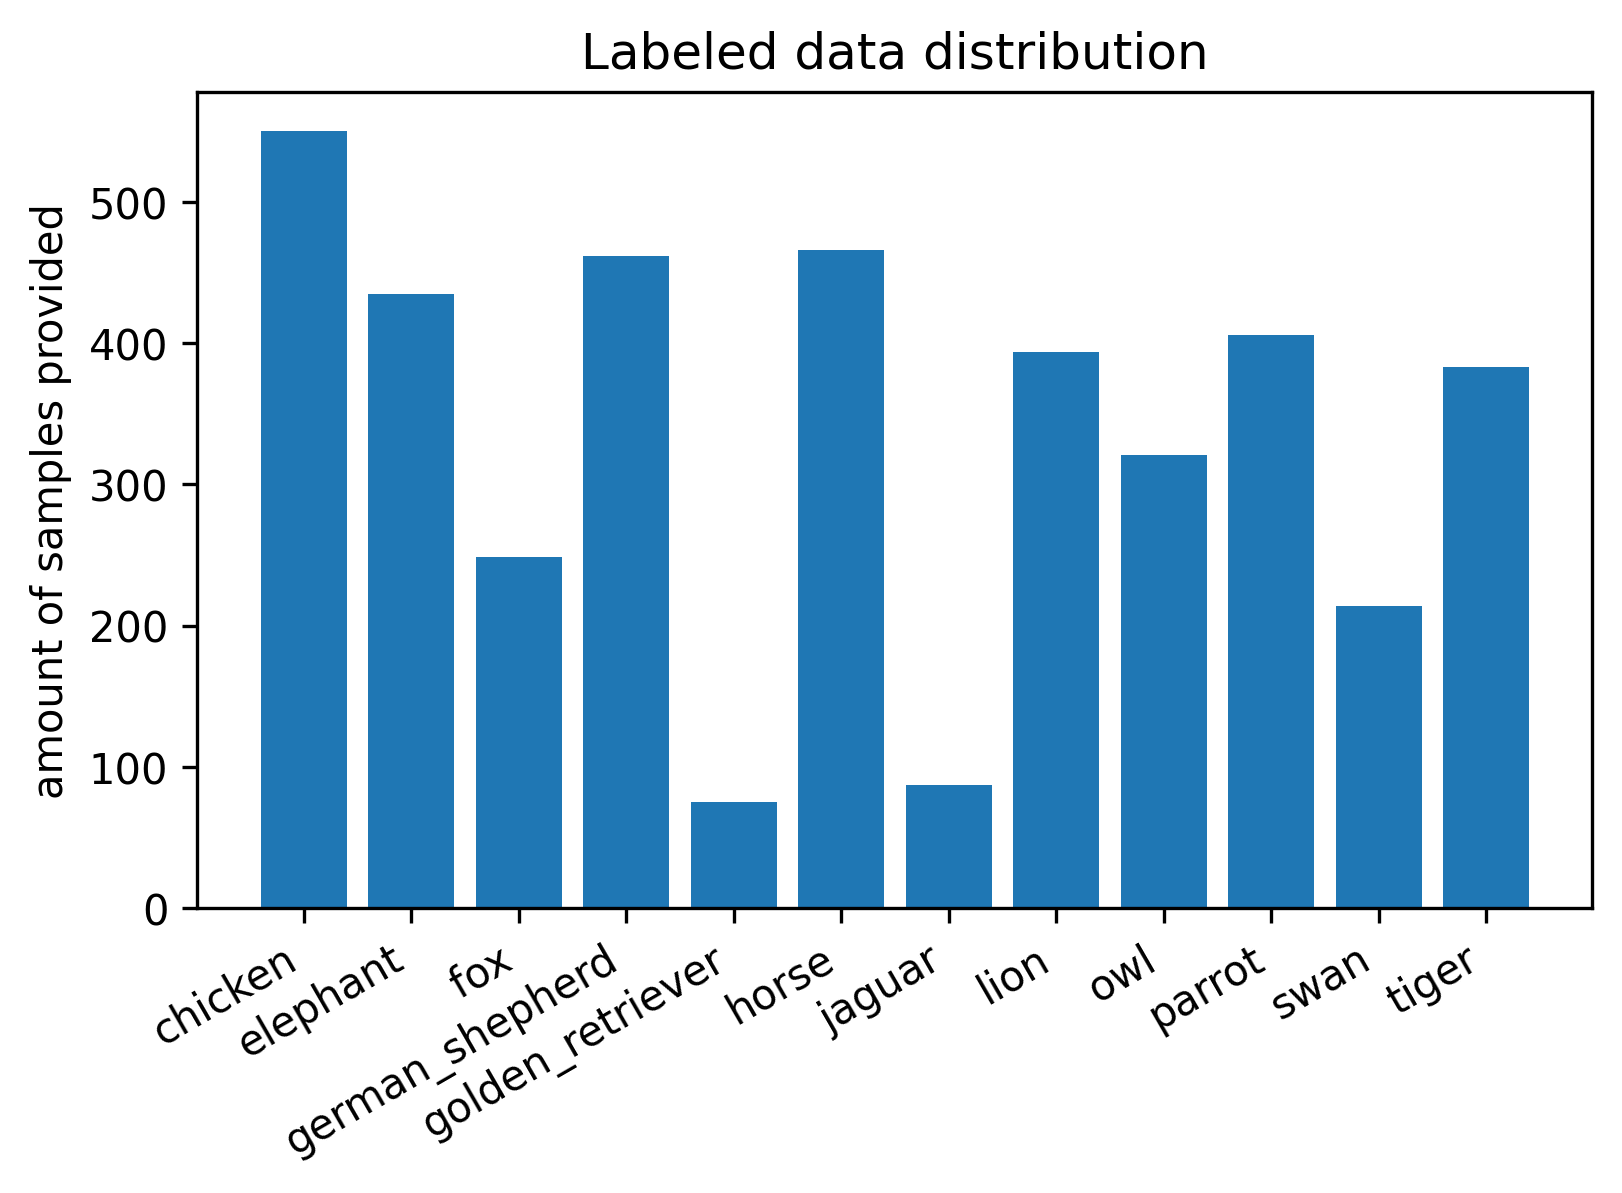
\includegraphics[width=0.7\linewidth]{images/1-data_analysis-labeled_data_distribution.png}}
    \captionsetup{width=0.65\linewidth}
    \captionsetup{justification=centering}
    \caption{The data distribution of the supplied training set.}
    \label{fig:1-data_analysis-labeled_data_distribution}
\end{figure}

%------------------------------------

\section{Deeper look at the training data}
\label{section:DA_deeper_look_data}

Whilst noting that the available data isn't balanced over all the classes is very important, there are also different aspects of the data that need analysing. 
An overview of the supplied training data is given in figure \ref{fig:1-data_analysis-labeled_data_overview.png}, available in the figures list at the end of this report.
This figure shows the first five images of each class.
From this, it becomes apparent that multiple factors of the data aren't \emph{optimal}.
This knowledge is important since it can aid in better prepossessing and in finding a better model in general.
The most noteworthy findings are listed here:
\begin{itemize}
    \item Images vary in shapes, some are taken in portrait, others in landscape.
    \item Images vary in size, some are high resolution whilst others are relatively low resolution.
    \item The framing of the subject(s) varies a lot. Sometimes the labelled animal is completely visible and centred in the frame. In some images there are multiple animals spread across the image, others show a close-up of the animal.
    \item Some images have a detailed background that makes up for a lot of the image, in others the background is blurry and its impact is presumably less.
    \item Some images have very vibrant colours in broad daylight, others are black and white in dimly lit environments.
\end{itemize}

This diversity in the provided training set is expected since it has been scraped from the web.
This also means that \emph{noise} can be expected, another important factor to keep in mind when choosing and optimizing models.
Many of the listed things can be minified by doing some clever prepossessing of the images.


%------------------------------------

\section{Feature extraction}
\label{section:DA_feature_extraction}

Since the focus of this competition is on developing great models and not necessarily on data prepossessing and feature extraction, some feature extraction has already been provided.
More info on the prepossessing and feature extraction provided is available in the provided notebook \emph{creating\_vbow.ipynb}.
In short, images are converted from there typical RGB representation to a numerical representation of interesting points, which can be used as input for our model.
How this is done will briefly be discussed here.

Instead of using the whole image as data, only a select few of \emph{interesting points} of the image are taken into consideration.
These interesting points of an image are found by using the \emph{Shi-Tomasi corner detector}.
The following important parameters for the \emph{features.extractShiTomasiCorners} function call are:
\begin{itemize}
    \item number of interesting points = 500
    \item minimum distance between interesting points = 20
\end{itemize}

Shown in figure \ref{fig:1-data_analysis-POI} is an example output of interesting points found by the Shi-Tomasi corner detector.
It's clear that this is far from optimal, but finding interesting points isn't an easy task and thus the results are better then they might seem on first sight.
This method might perform better after fine-tuning.

\begin{figure}[H]
    \centering
    \fbox{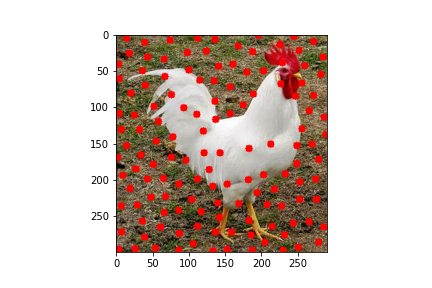
\includegraphics[width=0.8\linewidth]{images/1-data_analysis-POI.png}}
    \captionsetup{width=0.7\linewidth}
    \captionsetup{justification=centering}
    \caption{Example of points of interest found by Shi-Tomasi corner detector.}
    \label{fig:1-data_analysis-POI}
\end{figure}

Finding interesting points is only half of the work.
These interesting points now need to be represented by numerical values that have actual meaning, afterwards, they're clustered using a helper function.
Remember from section \ref{section:DA_deeper_look_data} that the provided images differ a lot.
Thus the numerical representation, generated by a descriptor, has to be so that it minifies the impact of different lighting, scaling...
The following descriptors are used and their outputs are provided: DAISY, ORB, FREAK, LUCID, VGG, BoostDesc, SIFT.
Whilst SURF is another great descriptor, it's not provided nor is the license available for this project.
SIFT is often referred to as the most famous and successful of these descriptors, but all of them should be explored.
Clustering is done by the \emph{createCodebook} function which uses Mini-Batch K-Means clustering from the SciKit Learn library.
This is also something that might be fine-tuned.

%------------------------------------

\section{The numerical representation}
\label{section:DA_numerical_representation}

As discussed in section \ref{section:DA_feature_extraction}, the images are stored as numerical representations using descriptors.
To save time, these numerical representations for all the descriptors are stored in a separate \emph{Pickle} file.
Since these representations form the input of a model, it's important to get a grip on how these look.
The provided \emph{createCodebook} function is used for clustering this data, which was also discussed in the previous section.
This function allows specifying how many clusters should be created for clustering the interesting points.
These different clusters can be thought of as different \emph{features}.
The function returns 2 lists.
The first contains the labels for the image represented at a certain index.
The other contains information about each image at that index.
This information is the output of the clustering done for that image and thus corresponds to an array which size equals the requested cluster amount.

An overview of the data from such clusters/features given by the SIFT descriptor is given in figure \ref{fig:1-data_analysis-labeled_data_overview.png}, available in the figures list at the end of this report.
From this, it is visible that the values seem to be normalized.
This would have to be checked for all descriptors used and perhaps some outliers would need to be removed.

In figure \ref{fig:1-data_analysis-correlation_matrix} the correlation matrix is shown for 30 clusters of the SIFT descriptor.
The correlation between these values doesn't seem too dramatic, which is mostly positive for our model building.
This is again something that would have to be checked for different parameters.

\begin{figure}[H]
    \centering
    \fbox{\includegraphics[width=0.8\linewidth]{images/1-data_analysis-correlation_matrix.png}}
    \captionsetup{width=0.7\linewidth}
    \captionsetup{justification=centering}
    \caption{Correlation matrix of 30 clusters made from the SIFT descriptor.}
    \label{fig:1-data_analysis-correlation_matrix}
\end{figure}

%START linear baseline model
\part{Linear baseline model}
\label{part:linear_baseline}

%------------------------------------

\section{About this part}
\label{section:LB_about_part}
TODO XXX



%START SVC
% done
\part{Support Vector Classifier}
\label{part:svc}

%------------------------------------

\section{About this part}
\label{section:SVC_about_part}

Now that a fine-tuned linear baseline model is established, the search for better models can start.
Sci Kit learn has a flow chart for deciding which estimator to use, \href{https://scikit-learn.org/stable/tutorial/machine_learning_map/index.html}{available here}.
When following this chart a Support Vector Classifier (SVC) is proposed, thus one is examined here.
Since part \ref{part:linear_baseline} already exhaustively discusses the model testing strategy used, this part will go into less detail to avoid repetition. 
The Notebook corresponding with this part is \texttt{support\_vector\_classifier.ipynb}.


%------------------------------------

\section{Scoring and methodology for fine-tuning}
\label{section:SVC_methodology}

Again, the multi-class Log Loss (MCLL) score is used to compare models.
\texttt{GridSearchCV} was used to find optimal parameters were no human reasoning is needed.
Figure \ref{fig:3-clusters} shows the results of experimenting with different clusters and descriptors.
It is noted that overfitting is clearly visible when using over 250 clusters.
For the final model SIFT with 100 clusters is used.

Balancing the class weight had a small positive impact, which is great!
The non-balanced one is discussed here but found parameters and reasoning are identical for both.
Making the toll more precise had a negligible impact (-0.00) on the results thus it is left default.
\texttt{GridSearchCV} was used to find the optima for C and gamma for the \textit{rbf}, \textit{sigmoid} and \textit{poly} kernel.
For the poly kernel, it was also used to find an optimal degree.
It was insured \texttt{GridSearchCV} uses Stratified K-Folds cross-validation (SCV) with MCLL scoring to keep the unbalance of classes in mind.
What follows are tested parameters and the found optimal for each of these experiments:
\begin{itemize}
    \item Rbf kernel
    \begin{itemize}
        \item Tested C: 0.001, 0.01 , 0.1, 0.5, 1.0, 1.5, 3, 5, 10 and 100.
        \item Tested gamma: "scale", "auto", 0.001, 0.01 , 0.1, 0.5, 1.0, 1.5, 3, 5, 10 and 100.
        \item Found optima: C = 1.5 | gamma = 0.01, auto or scale | SCV MCLL score of ± 1.46.
    \end{itemize}
    \item Sigmoid kernel
    \begin{itemize}
        \item Tested C: 0.001, 0.01 , 0.1, 0.5, 1.0, 1.5, 3, 5, 10 and 100.
        \item Tested gamma: "scale", "auto", 0.001, 0.01 , 0.1, 0.5, 1.0, 1.5, 3, 5, 10 and 100.
        \item Found optima: C = 5 or 10 | gamma = 0.001 | SCV MCLL score of ± 1.54.
    \end{itemize}
    \item Poly kernel:
    \begin{itemize}
        \item Tested C: 0.1, 0.5, 1.0, 1.5, 3 and 5.
        \item Tested gamma: "scale", "auto", 0.001, 0.01 , 0.1, 0.5, 1.0 and 1.5.
        \item Tested degree: 2, 3, 4, 5, 7 and 10.
        \item Found optima: C between 1 and 5 | degree = 3 | gamma = scale, auto or 0.01  | SCV MCLL score of ± 1.59.
    \end{itemize}
\end{itemize}

\begin{figure*}[ht]
    \centering
    \begin{subfigure}{.45\textwidth}
        \centering
        \fbox{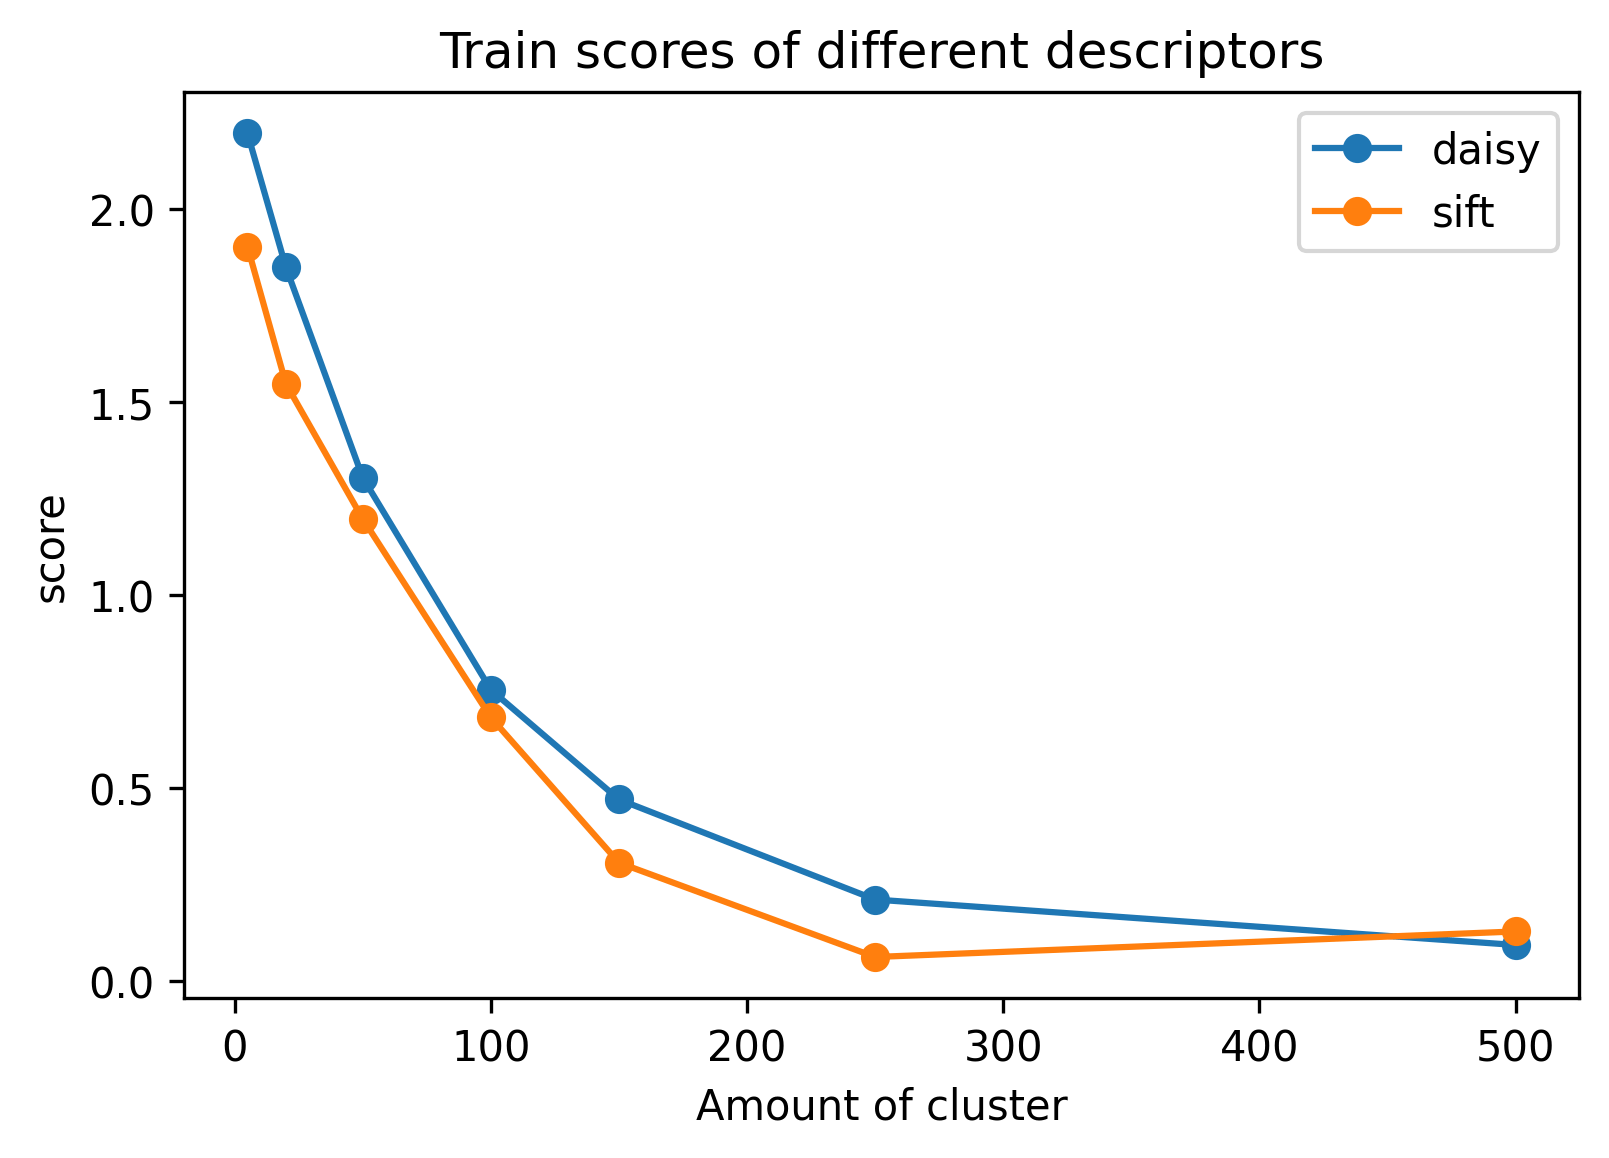
\includegraphics[width=\textwidth]{images/3/3_different_descriptors_train.png}}
        \captionsetup{width=0.9\linewidth}
        \captionsetup{justification=centering}
        \caption{Train scores.}
    \end{subfigure}
    \hspace{1cm}
    \begin{subfigure}{.45\textwidth}
        \centering
        \fbox{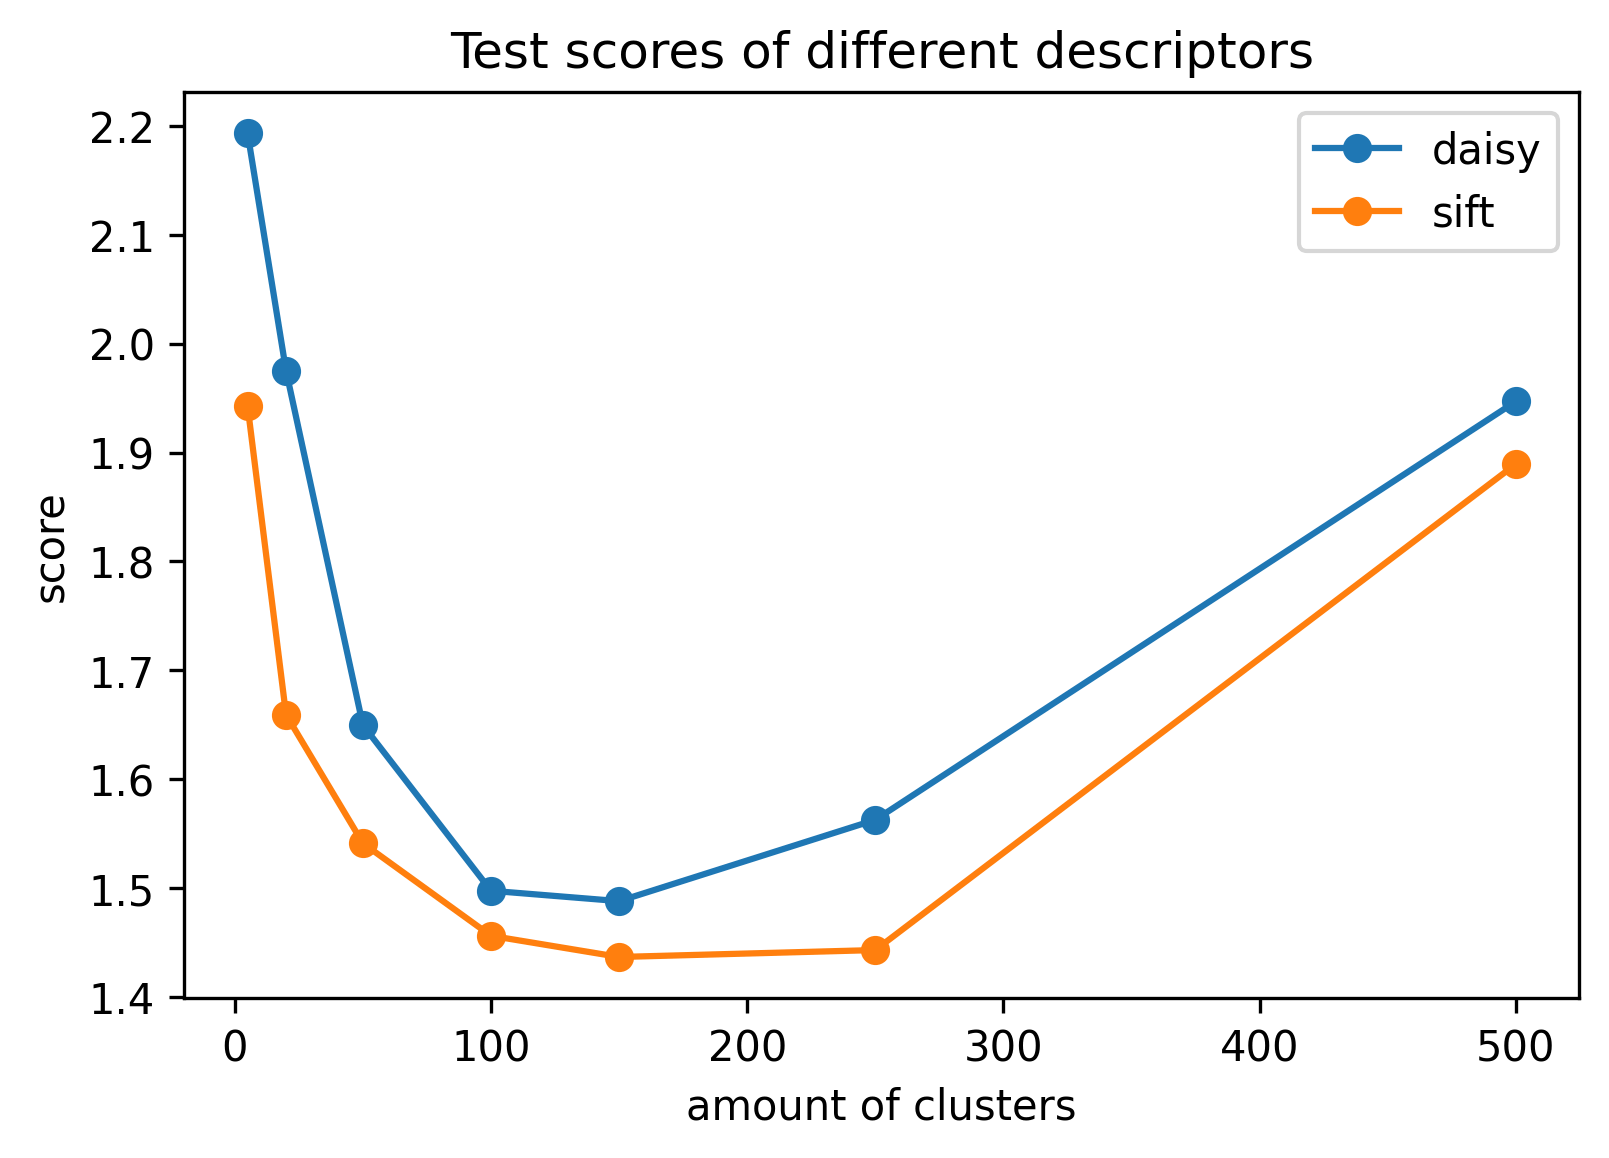
\includegraphics[width=\textwidth]{images/3/3_different_descriptors_test.png}}
        \captionsetup{width=0.9\linewidth}
        \captionsetup{justification=centering}
        \caption{Test scores.}
    \end{subfigure}
    \captionsetup{width=0.8\linewidth}
    \captionsetup{justification=centering}
    \caption{Averaged MCLL scores for optimal SVC model using different descriptors and clusters amounts over 3 trials. Lower score is better.}
    \label{fig:3-clusters}
\end{figure*}

\begin{wrapfigure}[13]{r}{0.6\textwidth}
    \centering
    \fbox{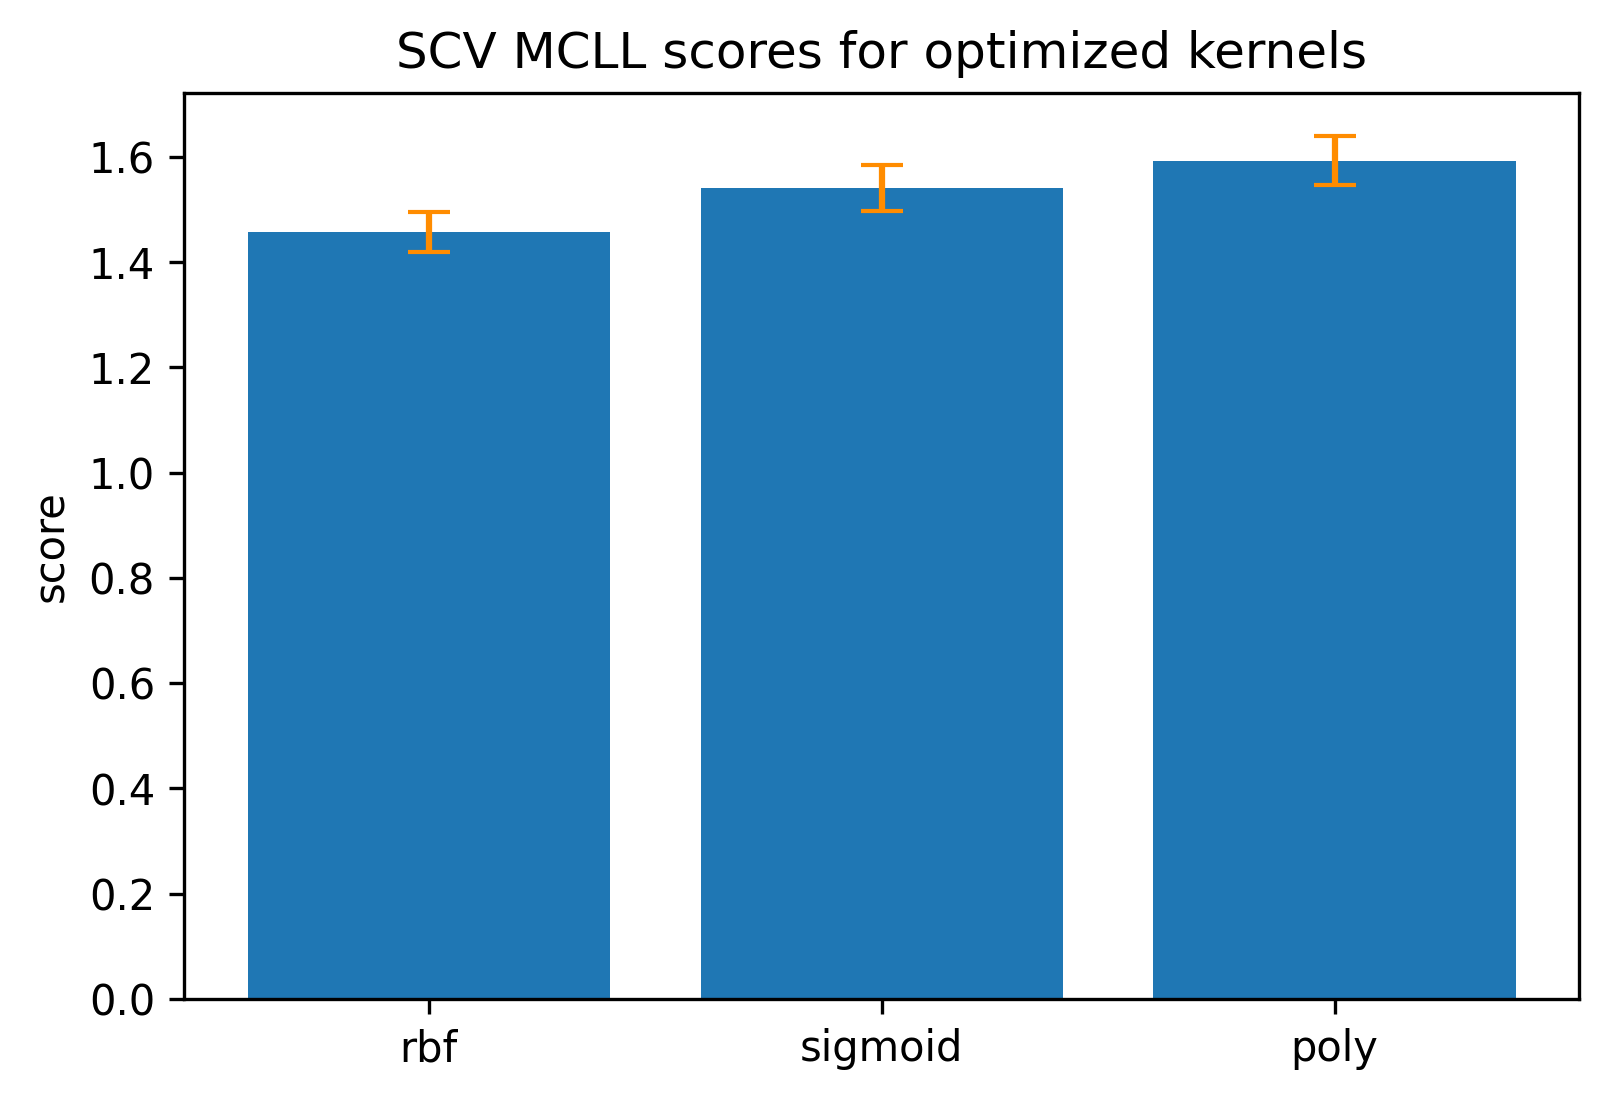
\includegraphics[width=0.75\linewidth]{images/3/SVC_optima_w_std.png}}
    \captionsetup{width=0.8\linewidth}
    \captionsetup{justification=centering}
    \caption{SCV MCLL score per kernel. \newline Lower score is better.}
    \label{fig:SVC_optima_w_std}
\end{wrapfigure}

A histogram showing the SCV MCLL score for each optimal kernel configuration together with the standard deviation is given in figure \ref{fig:SVC_optima_w_std}.
It is visible that the rbf kernel performed the best.
Thus, it was chosen to optimize this kernel further by doing another grid search that included more values around the found optima C and gamma.
The results from this further fine-tuning were negligible, C = 1.75 and gamma = 0.01 is used for the final model.

%------------------------------------

\section{The optimal settings for this model}
\label{section:svc_optimal}

The optimal settings and received score for the described model are:
\begin{itemize}
    \item Descriptor used: SIFT with 100 clusters
    \item Sample size for validation set: 15\%
    \item Class weight = balanced
    \item C =  1.75 | gamma = 0.01 | kernel = rbf | tol = 0.001
    \item MCLL score for validation set: ± 1.45 (balanced and unbalanced)
    \item SCV MCLL score: ± 1.48 (balanced and unbalanced)
    \item Score received on Kaggle: 1.55355 (non-balanced), 1.53626 (balanced)
\end{itemize}

%START linear SVC
% done
\part{Linear SVC}
\label{part:linear_svc}

%------------------------------------

\section{About this part}
\label{section:LinSVC_about_part}

In the previous part, three different kernels for SVC were explored.
Another kernel available for SVC is the \textit{linear kernel}.
However, there's also a separate model, \texttt{LinearSVC}, available as well.
The performance of the linear kernel and this separate model are explored in this part.
The Notebook corresponding with this part is \texttt{linear\_SVC.ipynb}.

%------------------------------------

\section{Scoring and methodology for fine-tuning}
\label{section:LinSVC_methodology}

The algorithms are tested and evaluated as the non-linear SVC from part \ref{part:svc}.
In order for MCLL scoring to work, a \texttt{predict\_proba} function should be available.
For \texttt{LinearSVC} this is not the case, it can, however, be implemented by wrapping it with Sci-Kit's \texttt{CalibratedClassifierCV}.
Arguably, this wrapping can influence the performance, however, the Kaggle competition also requires a \texttt{predict\_proba} function thus the wrapping is necessary and its performance impact should be taken into account.
Both balanced and non-balanced variant were considered, the received scores were comparable and the balanced variant is preferred and discussed.
A short discussion of the tried parameters and found results using \texttt{GridSearchCV} is listed here:
\begin{itemize}
    \item \texttt{SVC} with linear kernel:
    \begin{itemize}
        \item Tested C: 0.001, 0.01 , 0.1, 0.5, 1.0, 1.5, 3, 5, 10 and 100.
        \item Tested gamma: "scale", "auto", 0.001, 0.01 , 0.1, 0.5, 1.0, 1.5, 3, 5, 10 and 100.
        \item Found optima: C: 0.01 | gamma had no influence, 0.001 is chosen | SCV MCLL score of ± 1.56.
    \end{itemize}
    \item \texttt{LinearSVC}:
    \begin{itemize}
        \item Tested C: 0.001, 0.01 , 0.1, 0.5, 1.0, 1.5, 3, 5, 10 and 100.
        \item Tested penalty and loss: l1 and l2 | hinge and squared hinge.
        \item Tested dual: True and False.
        \item Found optima: C: 0.1 | penalty: l1 | dual: False | loss: squared hinge | SCV MCLL score of ± 1.63.
    \end{itemize}
\end{itemize}

%------------------------------------

\section{Linear is not the way to go}
\label{section:linsvc_optimal}

The SVC model with linear kernel performed better than the LinearSVC model.
Further fine-tuning around the found optima didn't gain any performance.
It is noted that LinearSVC often \textit{fitted quicker}, which perhaps explains it's existence.
Since the linear SVC approach performed worse then the optimal SVC found in part \ref{part:svc} it was not discussed in great detail and is not explored further.
Only SIFT with 100 clusters was tested.
During testing, the received MCLL score for the validation set was ± 1.60 and the SCV MCLL score was ± 1.55.
The received Kaggle score for the optimal linear SVC model is 1.59520.

%START random forest
% done
\part{Gradient Boosting}
\label{part:gradien_boost}

%------------------------------------

\section{About this part}
\label{section:gb_about_part}

All previous models where standalone classifiers, to make things more interesting an ensemble is tried next.
An ensemble consists of cleverly combining multiple \textit{weaker} classifiers to form a final \textit{strong} classifier.
Gradient Boosting and random forest are common ensembles.
A quick experiment showed that default Gradient Boosting performed better than an optimised random forest (MCLL of 1.68 vs 1.74).
Thus, it is chosen to only discuss Gradient Boosting further.
The Notebook corresponding with this part is \texttt{gradient\_boosting.ipynb}.

%------------------------------------

\section{Scoring and methodology for fine-tuning}
\label{section:gb_methodology}

Fine-tuning and evaluation of the model is done in an equal manner as the previous models.
This model doesn't have a parameter like class weight which specifies to work in a balanced manner.
Due to the many parameters that need fine-tuning and limited computing power, the use of \texttt{GridSearchCV} was split over 2 independent searches.
Found optima were retested to validate they don't influence previous determined parameters.
The tried parameters using \texttt{GridSearchCV} are listed here:
\begin{itemize}
    \item Experiment 1:
    \begin{itemize}
        \item Tested loss: deviance and exponential.
        \item Tested learning rates: 0.001, 0.01 , 0.1 and 0.5.
        \item Tested amount of estimators: 50, 100, 250, 500, 600, 750 and 1000.
    \end{itemize}
    \item Experiment 2:
    \begin{itemize}
        \item Tested subsample: 0.5, 0.75, 1.0 and 1.5.
        \item Tested minimum sample split: 2, 3 and 5.
        \item Tested max depth: 3, 5, 7 and 10.
    \end{itemize}
\end{itemize}

%------------------------------------

\section{Interesting but not impressive}
\label{section:gb_optimal}

Whilst the Gradient Boosting approach is interesting, it didn't score well and there are signs of overfitting with an MCLL score of ± 0.21 on the training data using some settings.
The latter could perhaps be resolved but since the model performed worse than the linear baseline model throughout testing, it was not explored further.
Only SIFT with 100 clusters was considered.
A MCLL score of ± 1.68 on the validation set, a SCV MCLL score of ± 1.62 and a Kaggle score of 1.70494 were achieved with the following parameters:
\begin{itemize}
    \item Loss and learning rate: deviance and 0.01.
    \item Amount of estimators and subsample: 750 and 0.75.
    \item Minimum sample split and max depth: 5.
\end{itemize}

%START MA
% done
\part{Model analysis}
\label{part:model_anal}

%------------------------------------

\section{About this part}
\label{section:ma_about_part}

In the previous parts, many different models were developed and the most interesting ones were discussed.
This part will analyse these models by briefly discussing the confusion matrices.
The learning curves don't tell much but they are included in the extra figures list for completeness.
The Notebook corresponding with this part is \texttt{model\_analysis.ipynb}.

%------------------------------------

\section{Non-balanced Linear baseline model}
\label{section:ma_lbm_nonb}

The confusion matrices given in figure \ref{fig:ma_lbm_cm} teaches us multiple things, the most important of which are listed here:
\begin{itemize}
    \item Even though the jaguar class had very few examples, it classifies considerably well.
    \item The classifier completely fails in classifying the fox class even though the unbalance of the class wasn't so drastic. It also completely fails in classifying golden retriever, which was heavily unbalanced.
    \item An owl is more mistaken for a parrot then vice versa. 
    \item The model prefers classes which have a higher frequency when uncertain.
\end{itemize}

\begin{figure*}[ht]
    \centering
    \begin{subfigure}{.45\textwidth}
        \centering
        \fbox{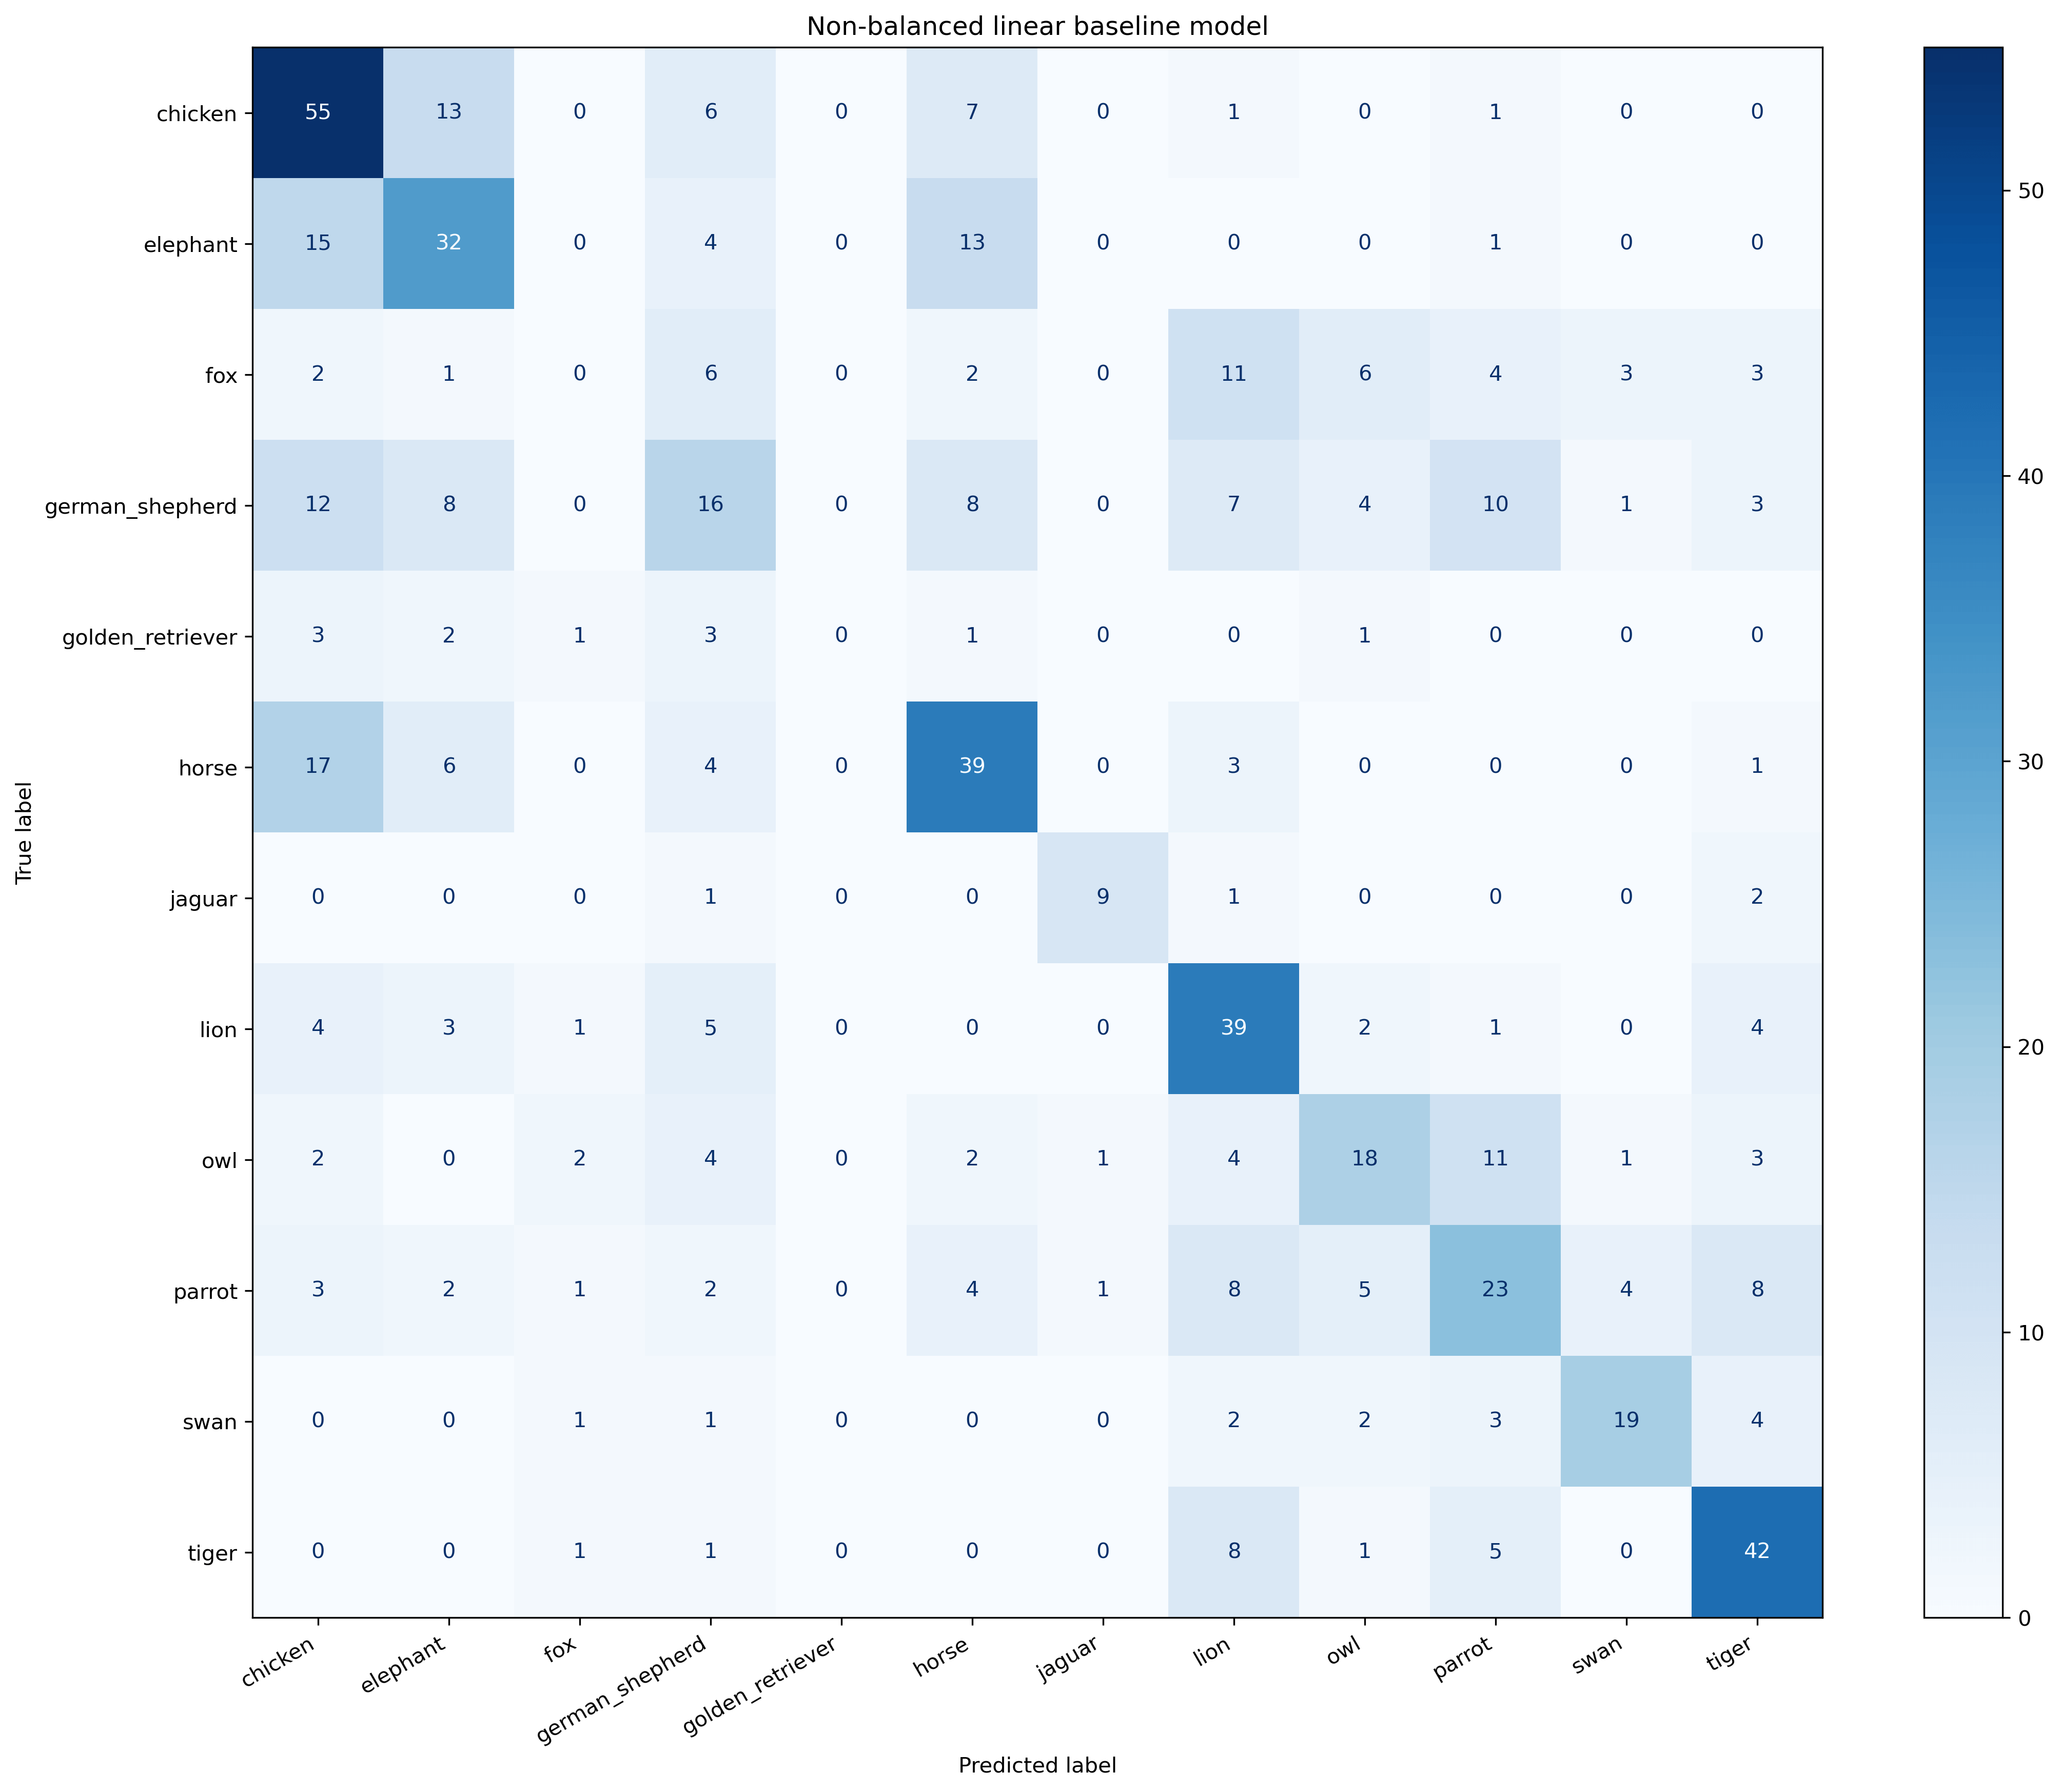
\includegraphics[width=\textwidth]{images/MA/MA_LBM_non_normalised.png}}
        \captionsetup{width=0.9\linewidth}
        \captionsetup{justification=centering}
        \caption{Non normalised CM.}
    \end{subfigure}
    \hspace{1cm}
    \begin{subfigure}{.45\textwidth}
        \centering
        \fbox{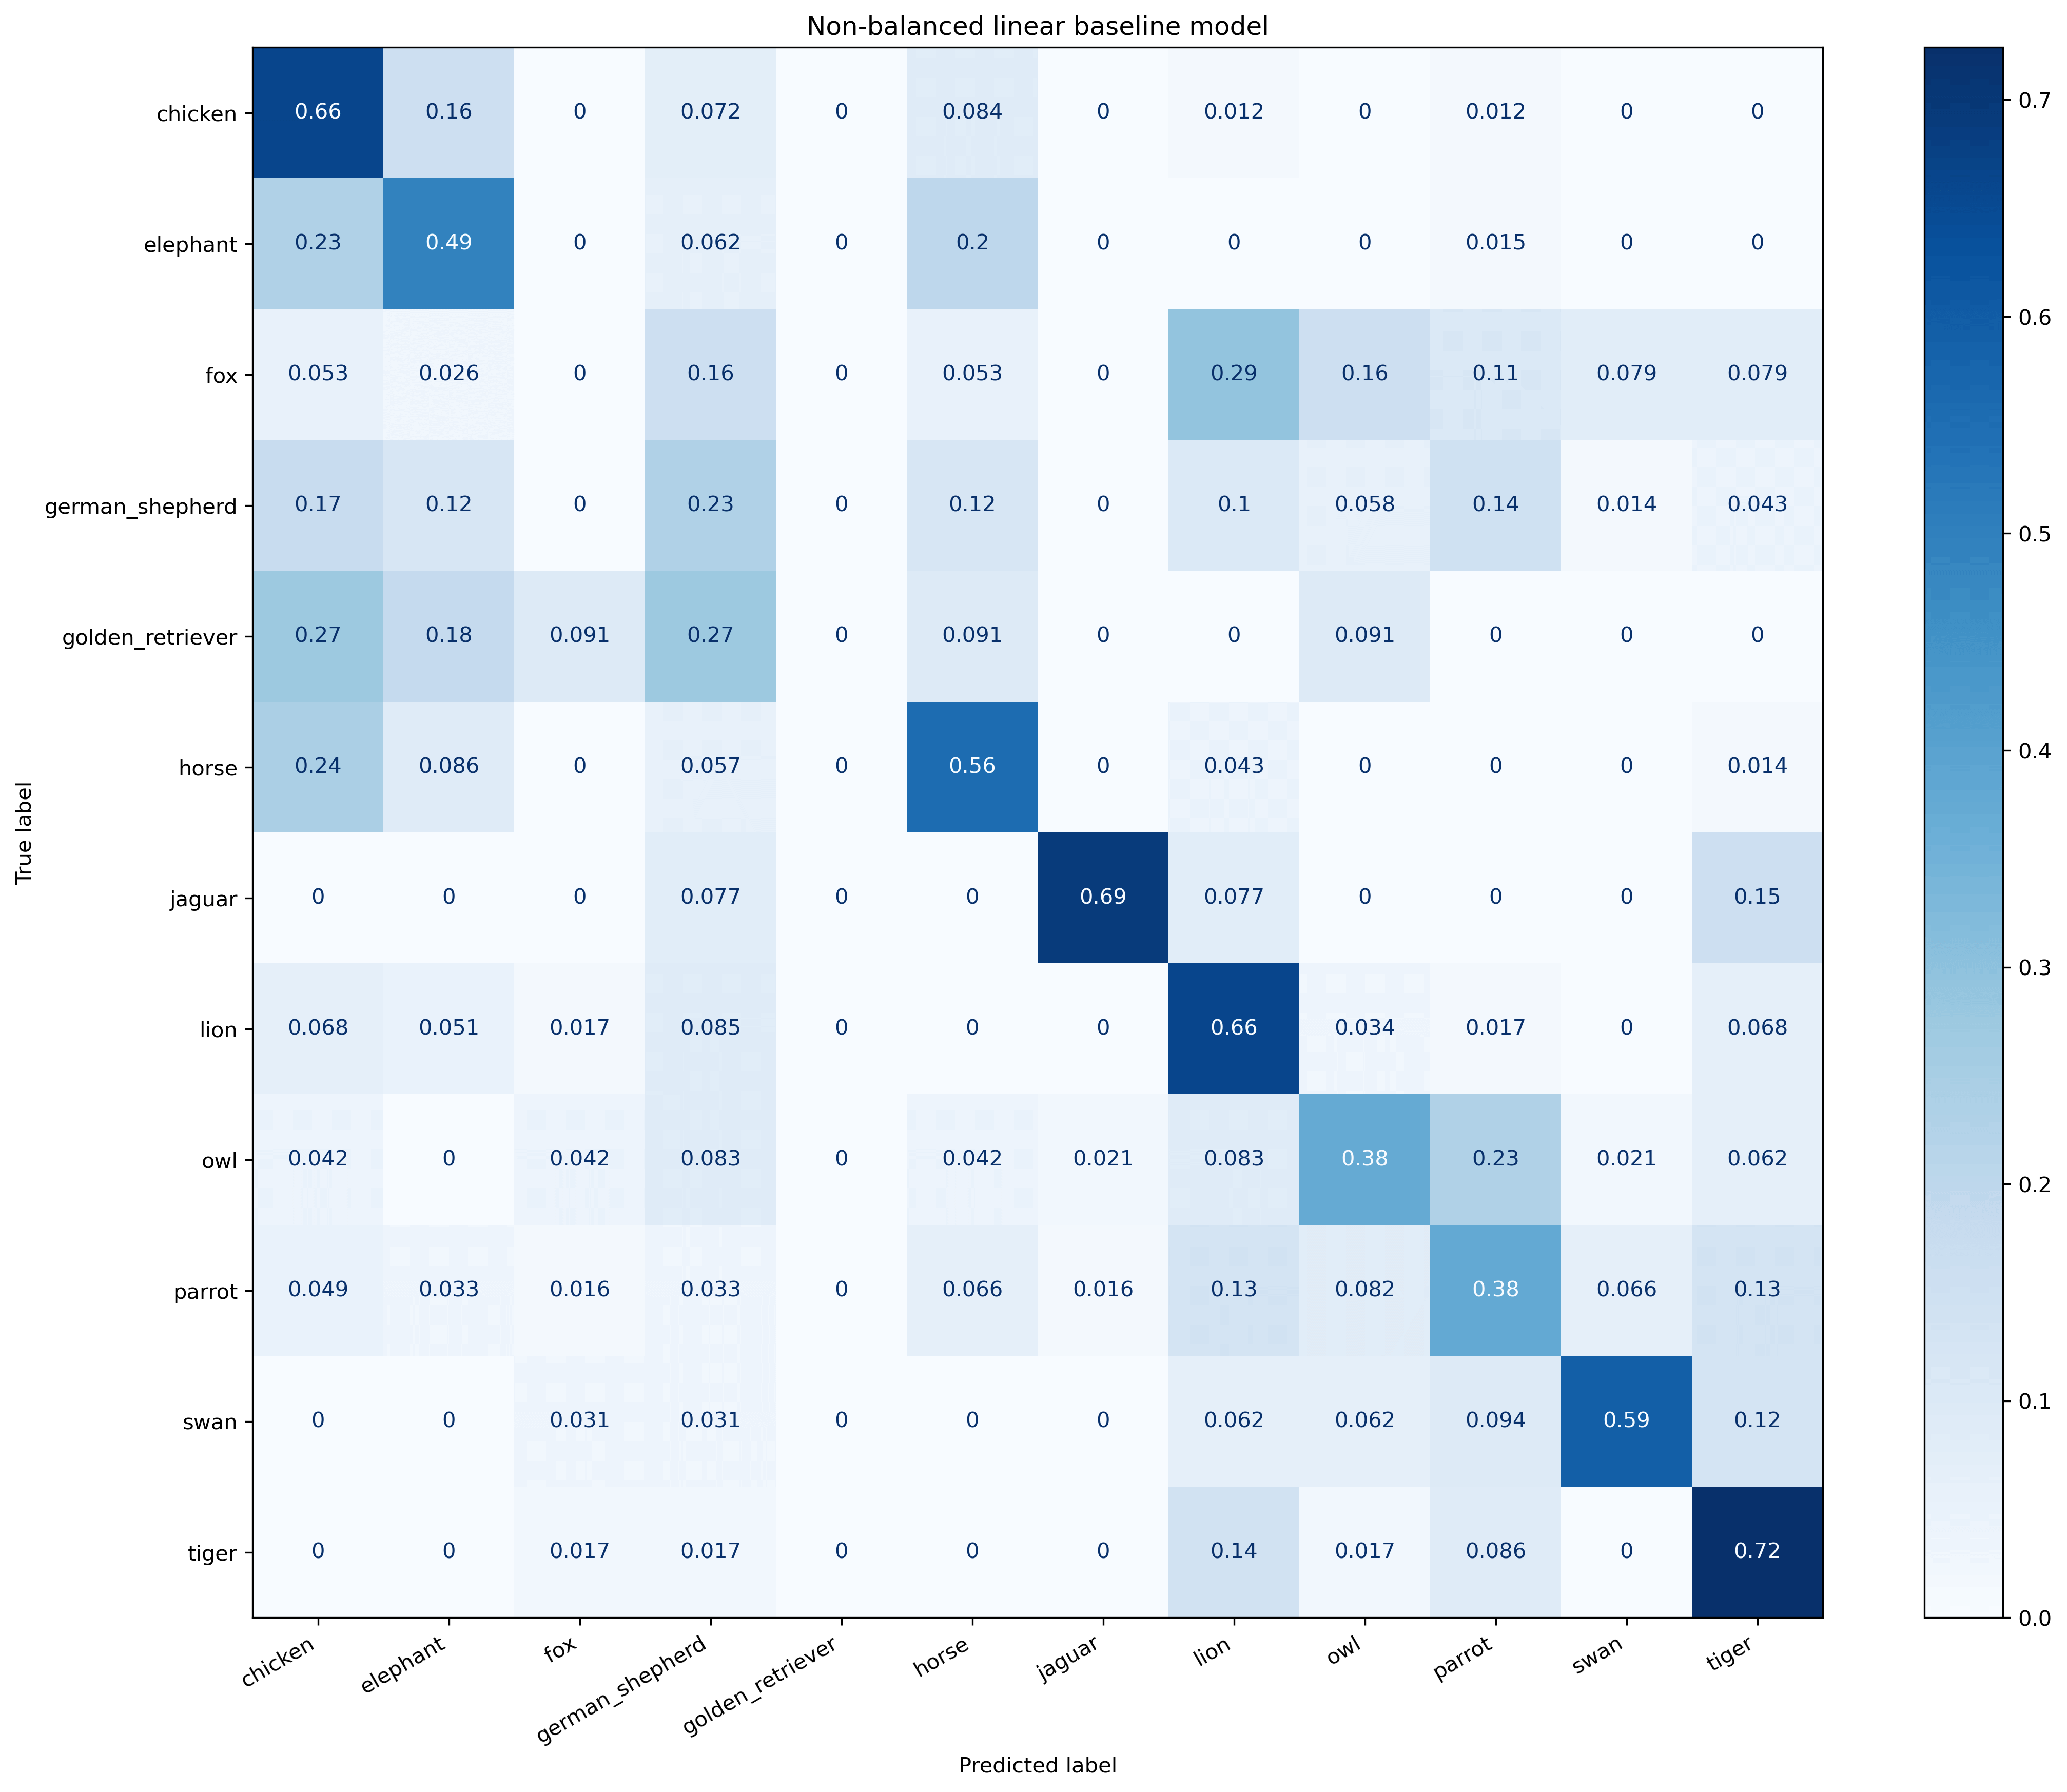
\includegraphics[width=\textwidth]{images/MA/MA_LBM_normalised.png}}
        \captionsetup{width=0.9\linewidth}
        \captionsetup{justification=centering}
        \caption{Normalised CM.}
    \end{subfigure}
    \captionsetup{width=0.8\linewidth}
    \captionsetup{justification=centering}
    \caption{Confusion matrices for the non-balanced linear baseline model.}
    \label{fig:ma_lbm_cm}
\end{figure*}

%------------------------------------

\section{Balanced linear baseline model}
\label{section:ma_lbm_balanced}

It was said in section \ref{section:LBM_finetuning_model} that it was weird the balanced LBM model received a worse MCLL score.
The confusion matrices given in figure \ref{fig:ma_lbm_cm_bal} shows a different story and teaches us multiple things, the most important of which are listed here:
\begin{itemize}
    \item The model now has some succession for each class, all be it low. This behaviour is more preferred and whilst it had a worse MCLL score it's confusion matrix shows it had a better understanding of the problem. The worse MCLL score is most likely due to the unbalance in the test set and when using CSV, the worse Kaggle score suggest the test data for the public leaderboard is also unbalanced.
    \item The correct classification of most classes has risen. These few that have dropped are classes with a high frequency suggesting it's better labelling was based on frequency bias instead of conceptual understanding for the non-balanced model. 
\end{itemize}

\begin{figure*}[ht]
    \centering
    \begin{subfigure}{.45\textwidth}
        \centering
        \fbox{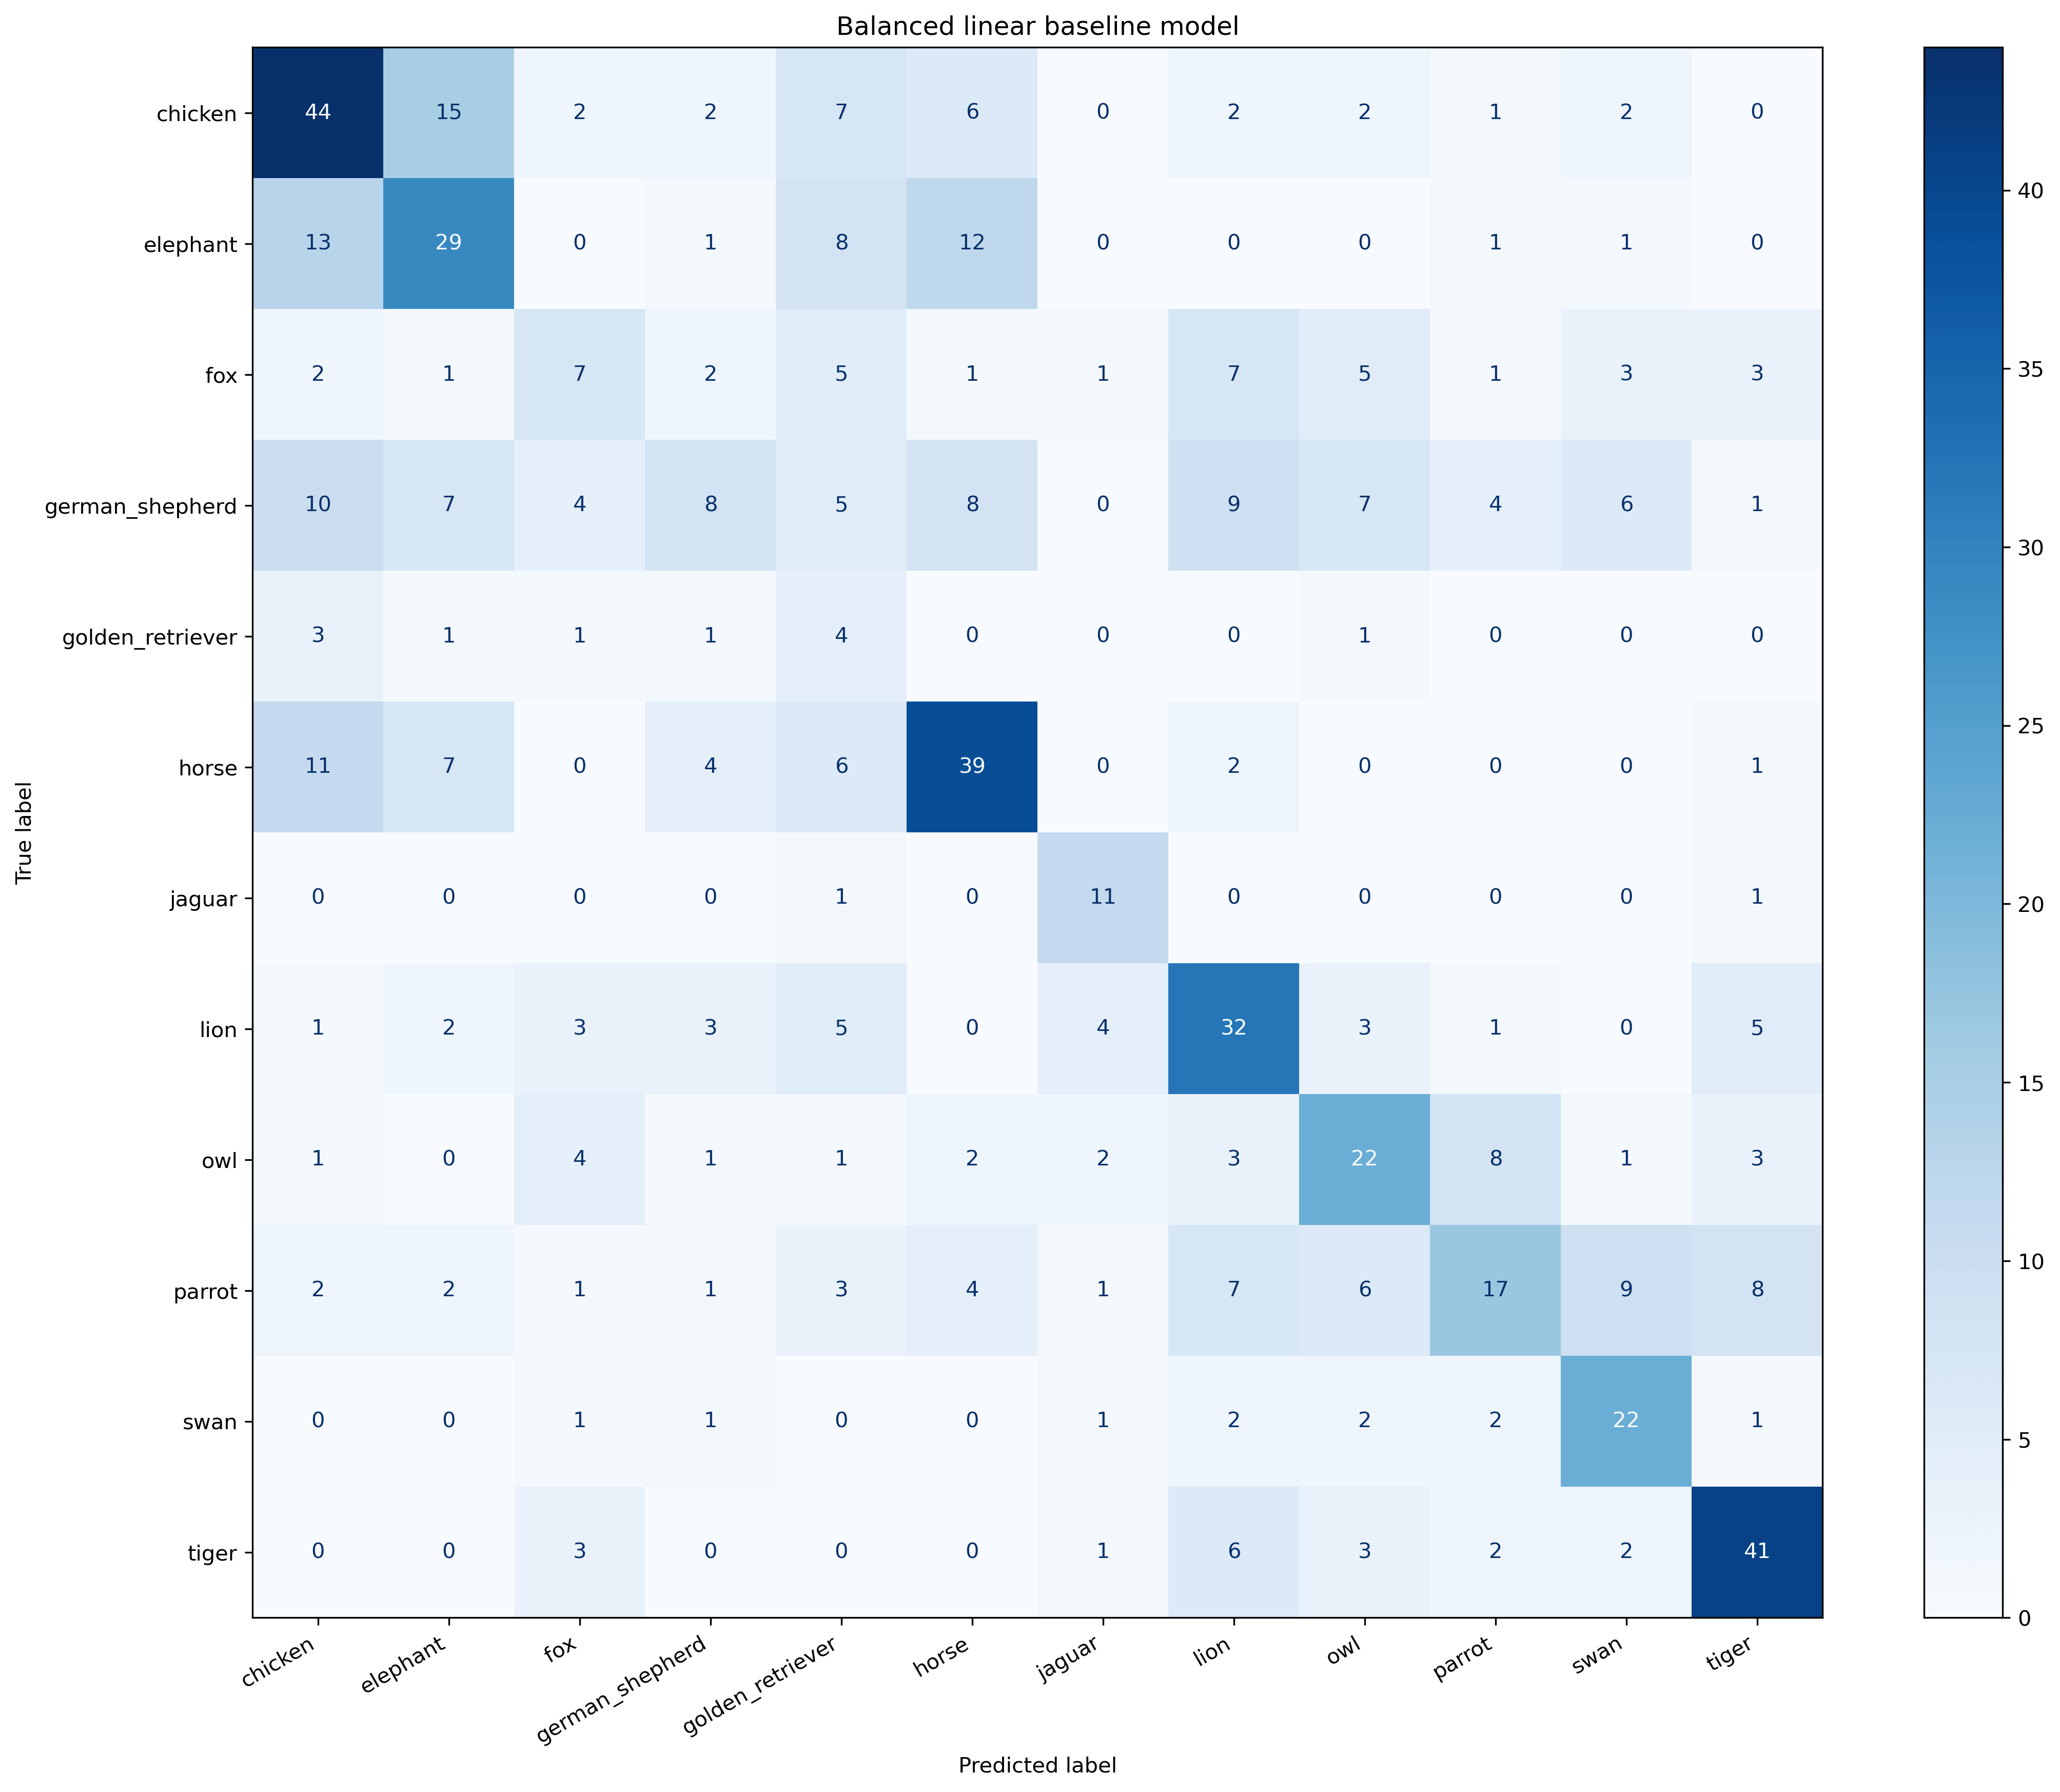
\includegraphics[width=\textwidth]{images/MA/MA_LBM_non_normalised_balanced.png}}
        \captionsetup{width=0.9\linewidth}
        \captionsetup{justification=centering}
        \caption{Non normalised CM.}
    \end{subfigure}
    \hspace{1cm}
    \begin{subfigure}{.45\textwidth}
        \centering
        \fbox{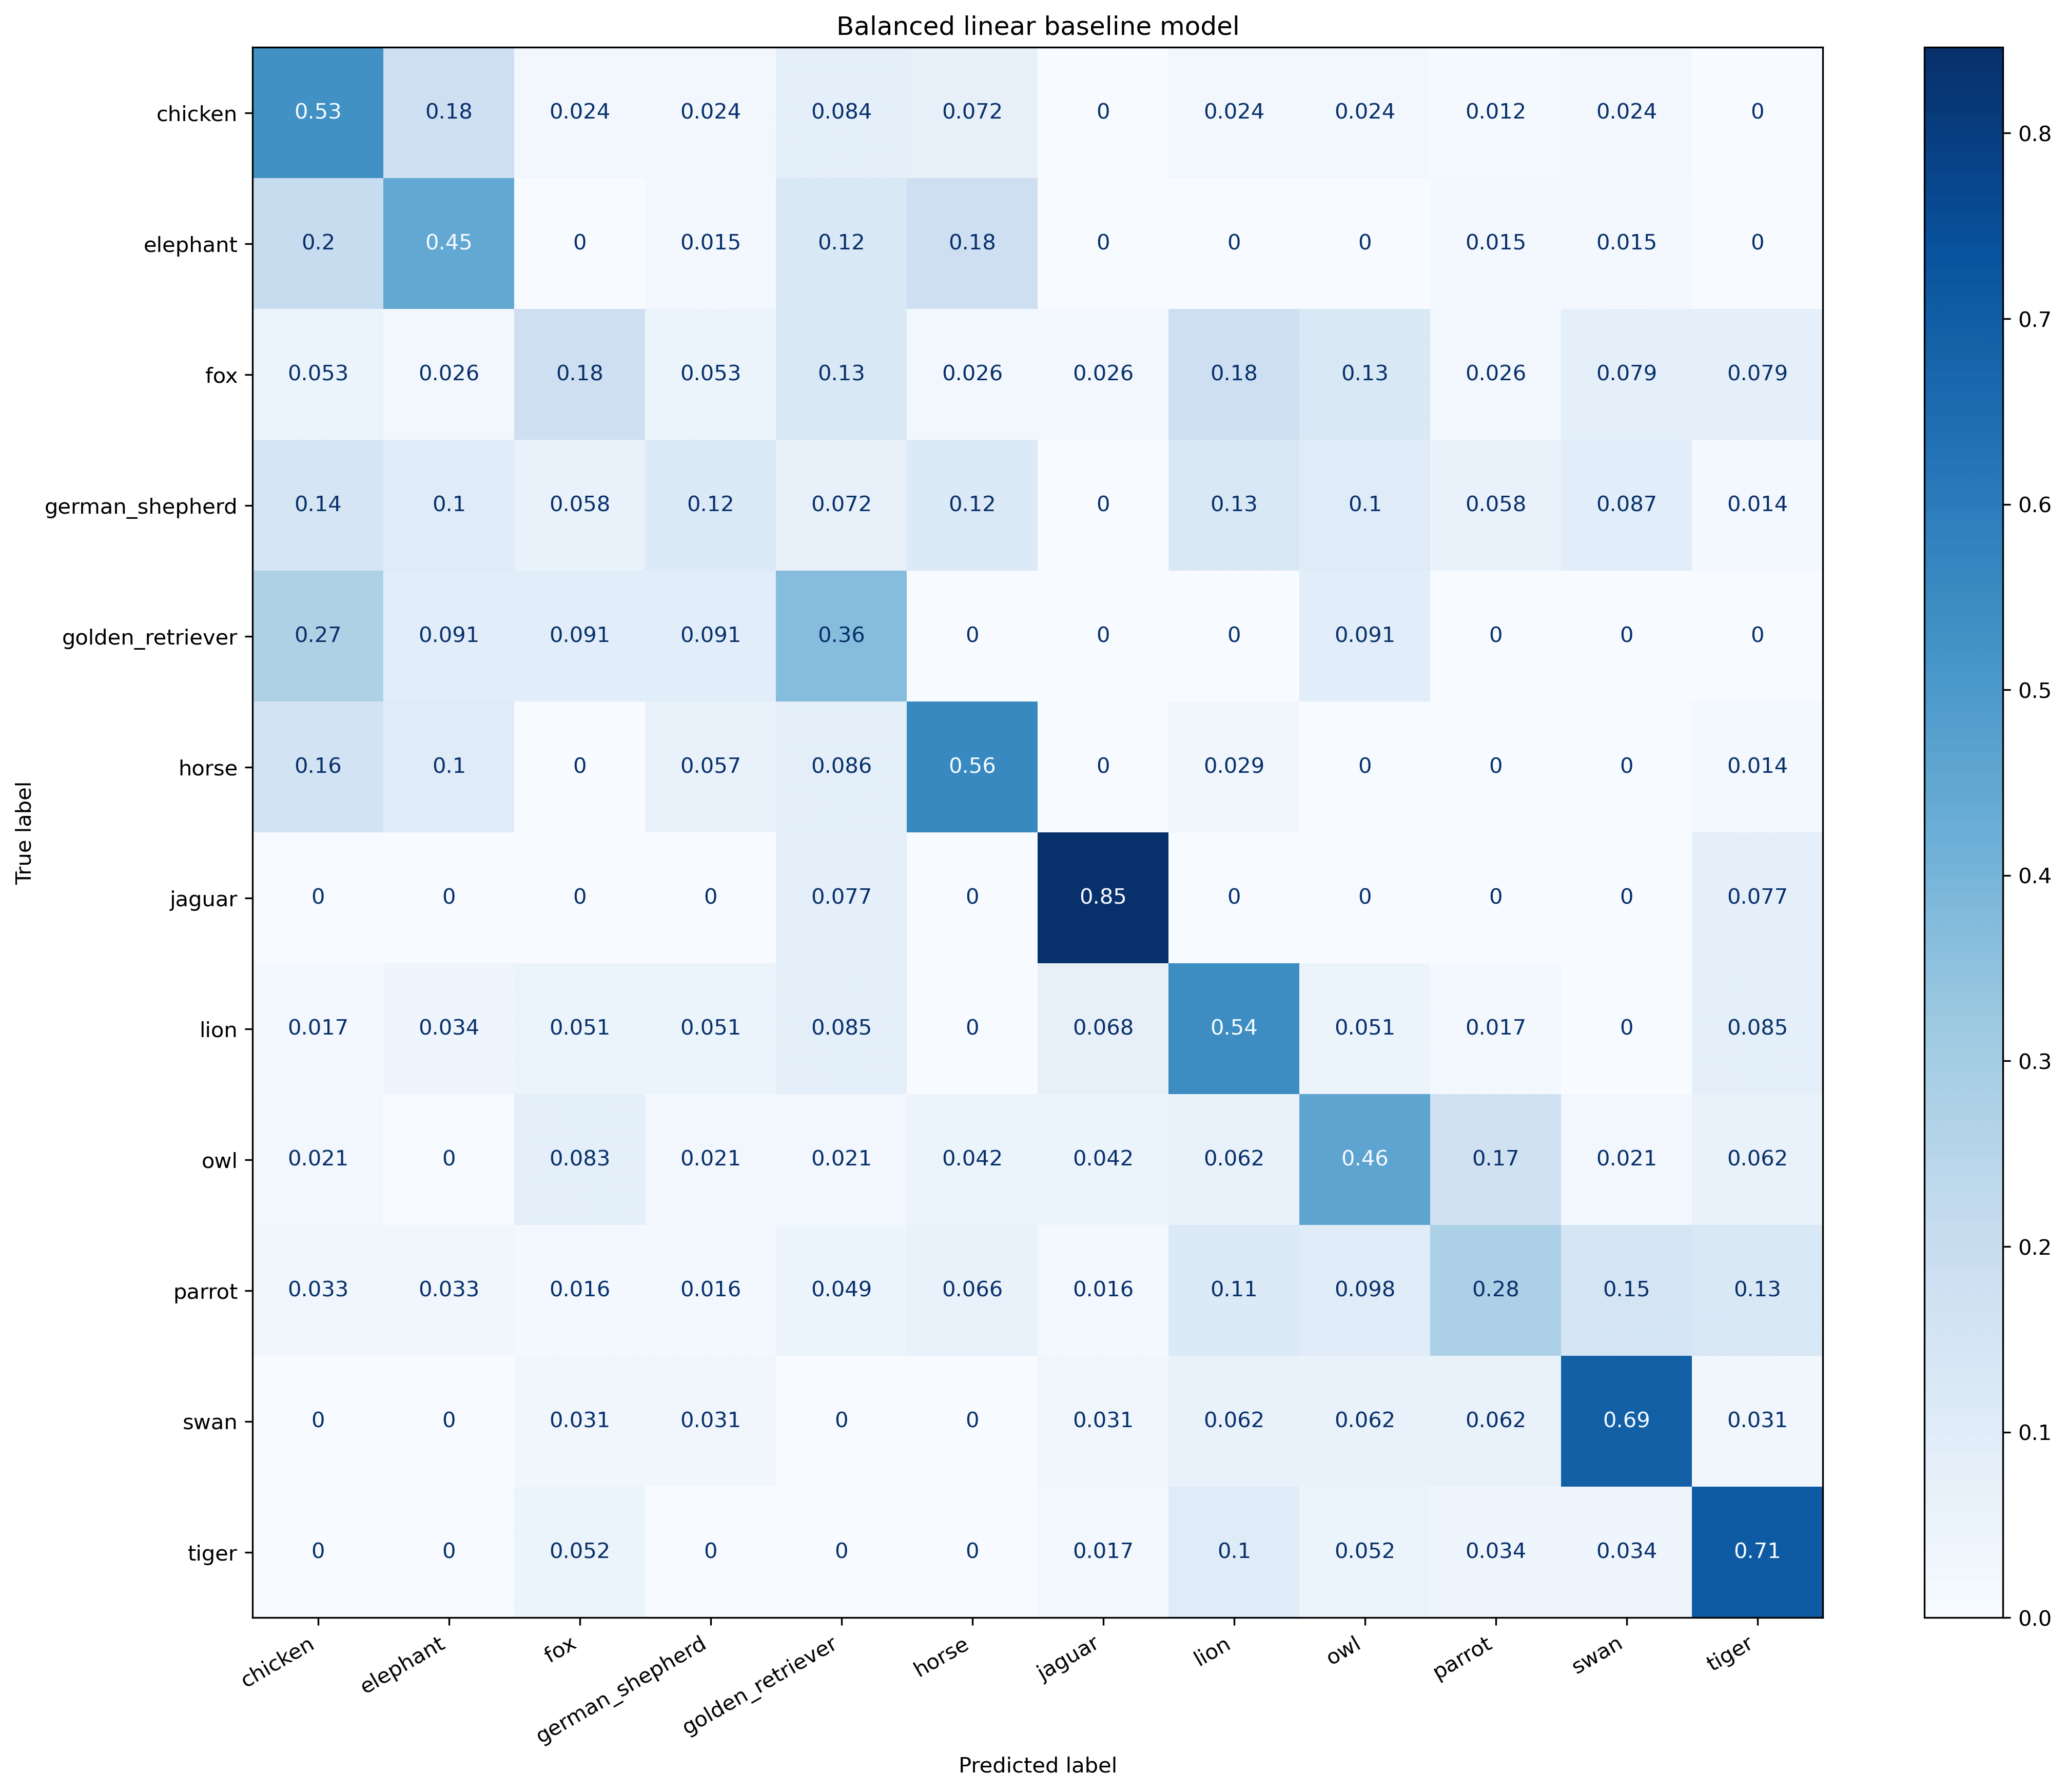
\includegraphics[width=\textwidth]{images/MA/MA_LBM_normalised_balanced.png}}
        \captionsetup{width=0.9\linewidth}
        \captionsetup{justification=centering}
        \caption{Normalised CM.}
    \end{subfigure}
    \captionsetup{width=0.8\linewidth}
    \captionsetup{justification=centering}
    \caption{Confusion matrices for the balanced linear baseline model.}
    \label{fig:ma_lbm_cm_bal}
\end{figure*}

%------------------------------------

\section{Support Vector Classifier model}
\label{section:ma_svc_balanced}

The Support Vector Classifier model was the best performing model.
This is shown in figure \ref{fig:ma_svc_cm} where the correct classification is considerably better than with the LBM. There are some important notes to be made:
\begin{itemize}
    \item The model is considerably worse at identifying golden retrievers and swans compared to the balanced LBM.
    \item The model outperforms the non-balanced LBM for almost all classes but classifying dogs and swans remains a difficult task.
    \item When wrongly classifying, the made error is comparable to the one for the balanced LBM, e.g. a fox is often misinterpreted as a lion. This suggests there's a correlation between these classes.
\end{itemize}

\begin{figure*}[ht]
    \centering
    \begin{subfigure}{.45\textwidth}
        \centering
        \fbox{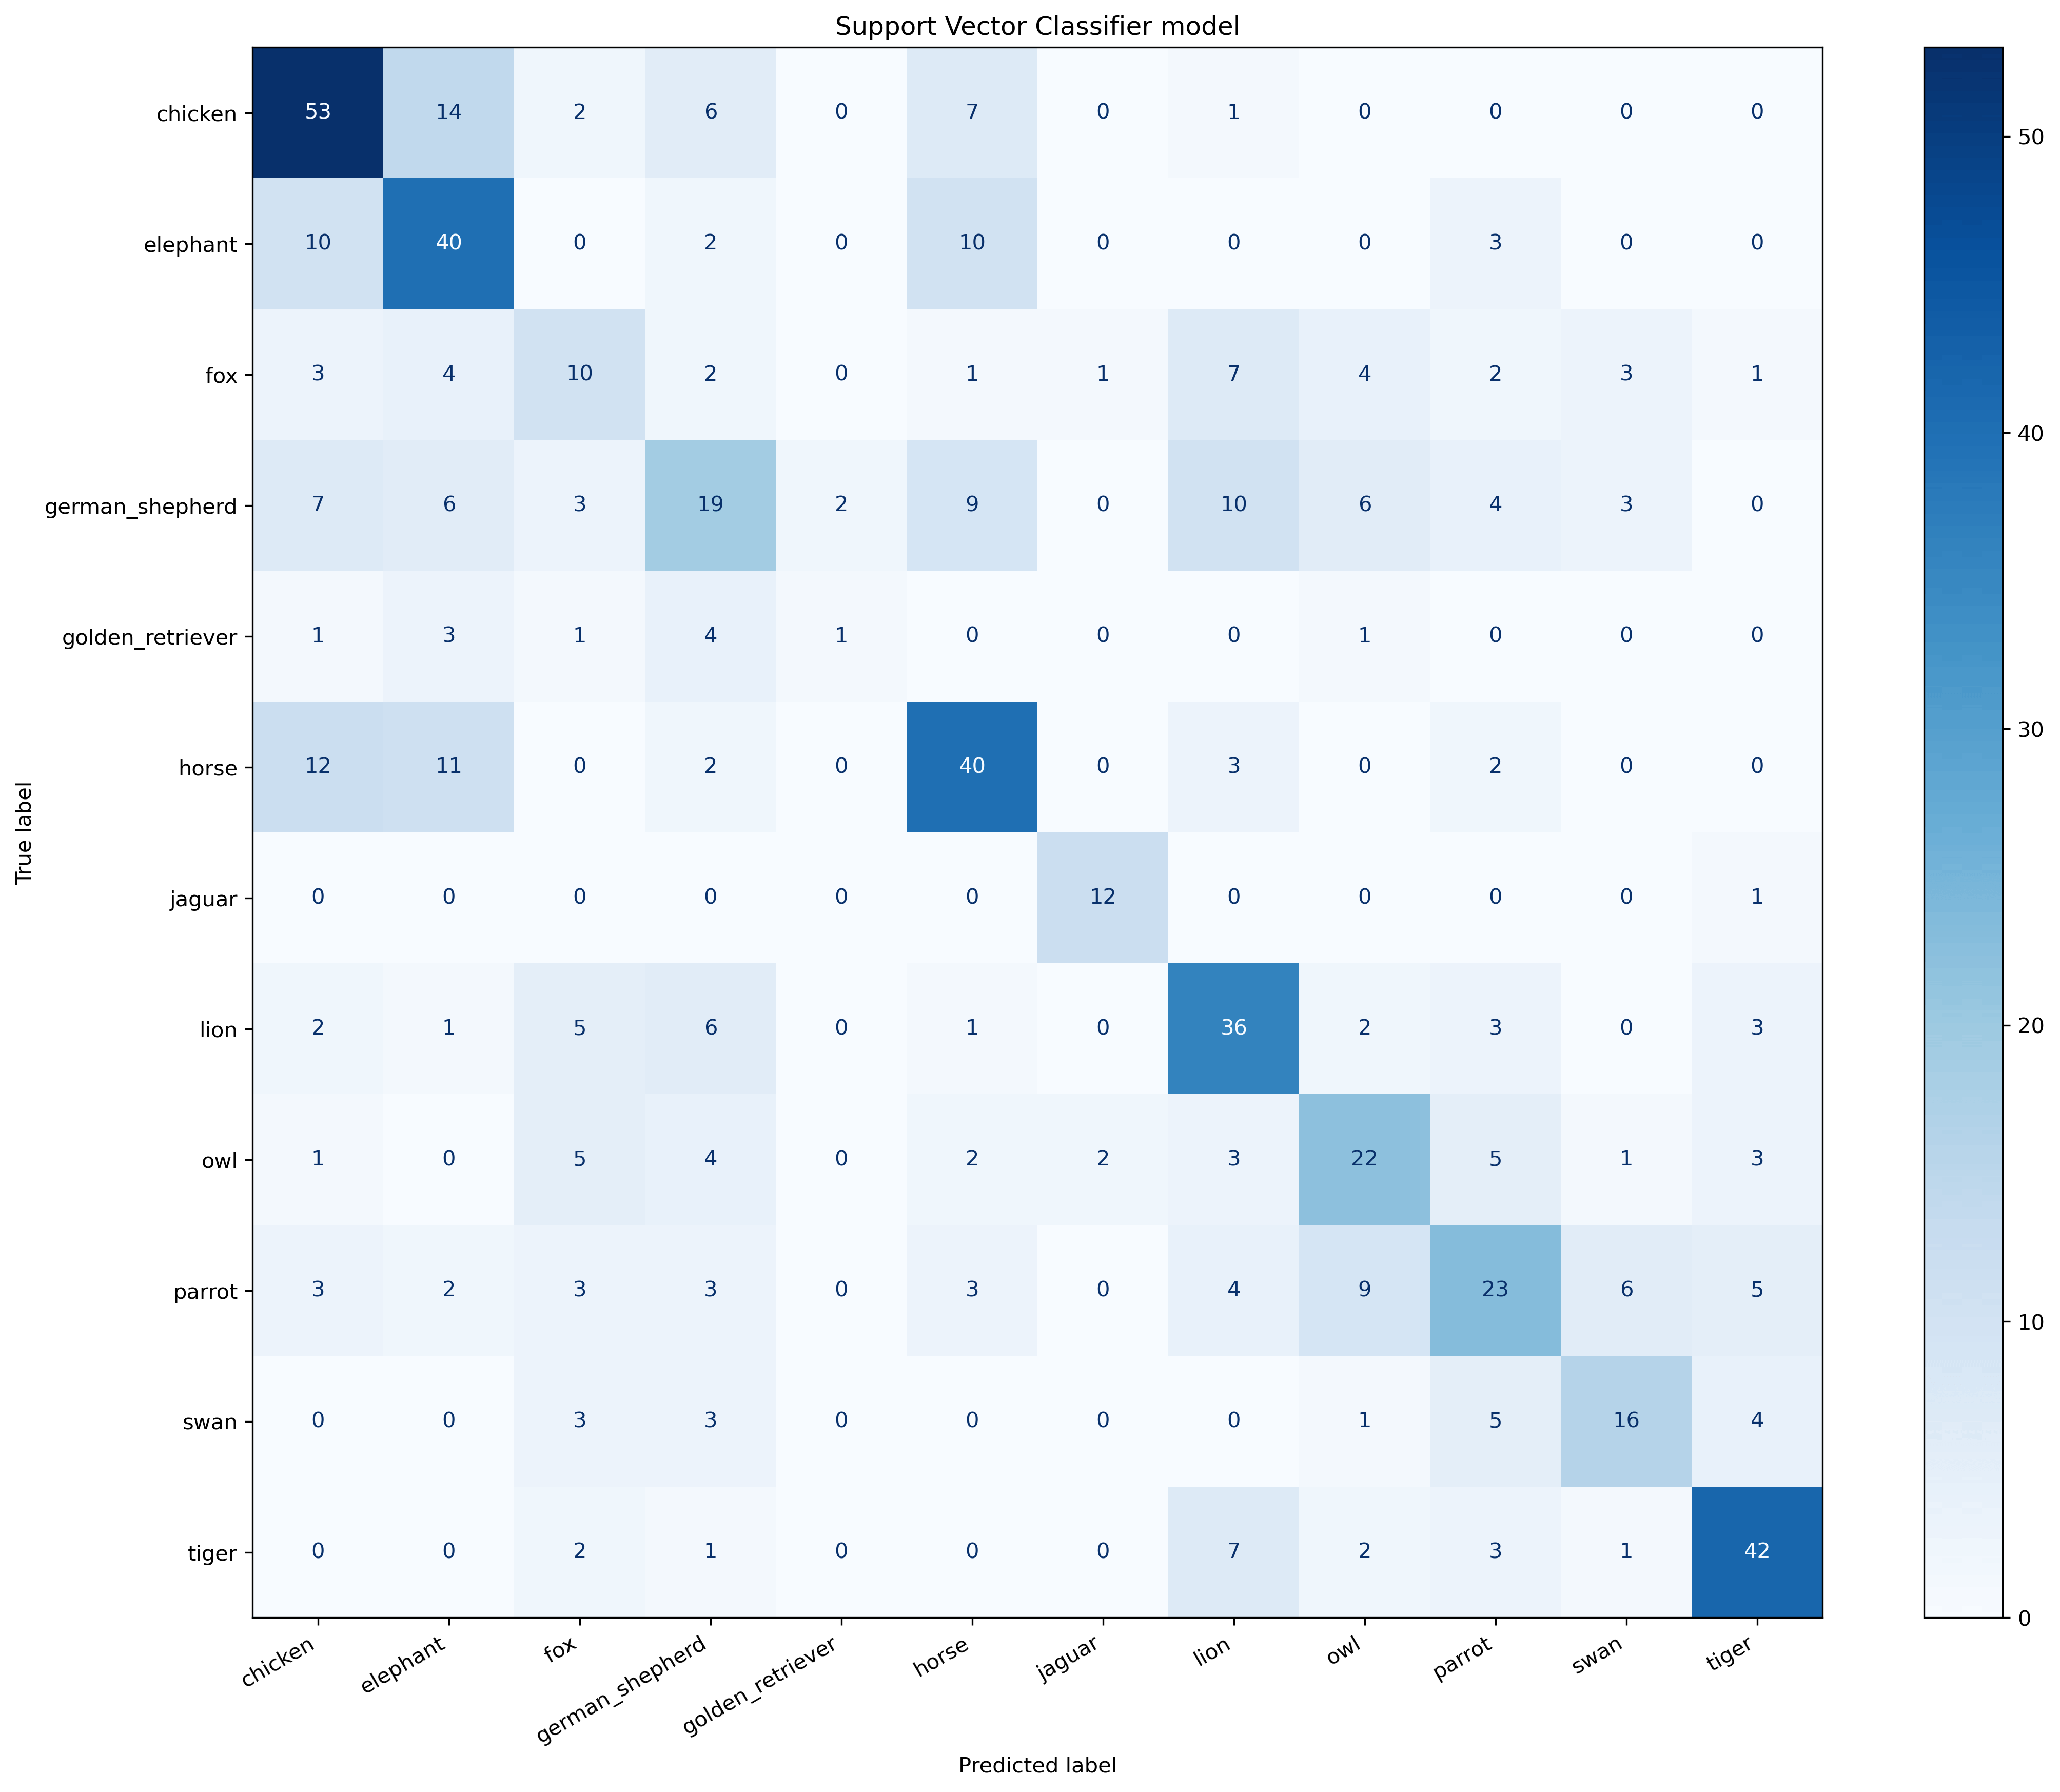
\includegraphics[width=\textwidth]{images/MA/MA_SVC_non_normalised.png}}
        \captionsetup{width=0.9\linewidth}
        \captionsetup{justification=centering}
        \caption{Non normalised CM.}
    \end{subfigure}
    \hspace{1cm}
    \begin{subfigure}{.45\textwidth}
        \centering
        \fbox{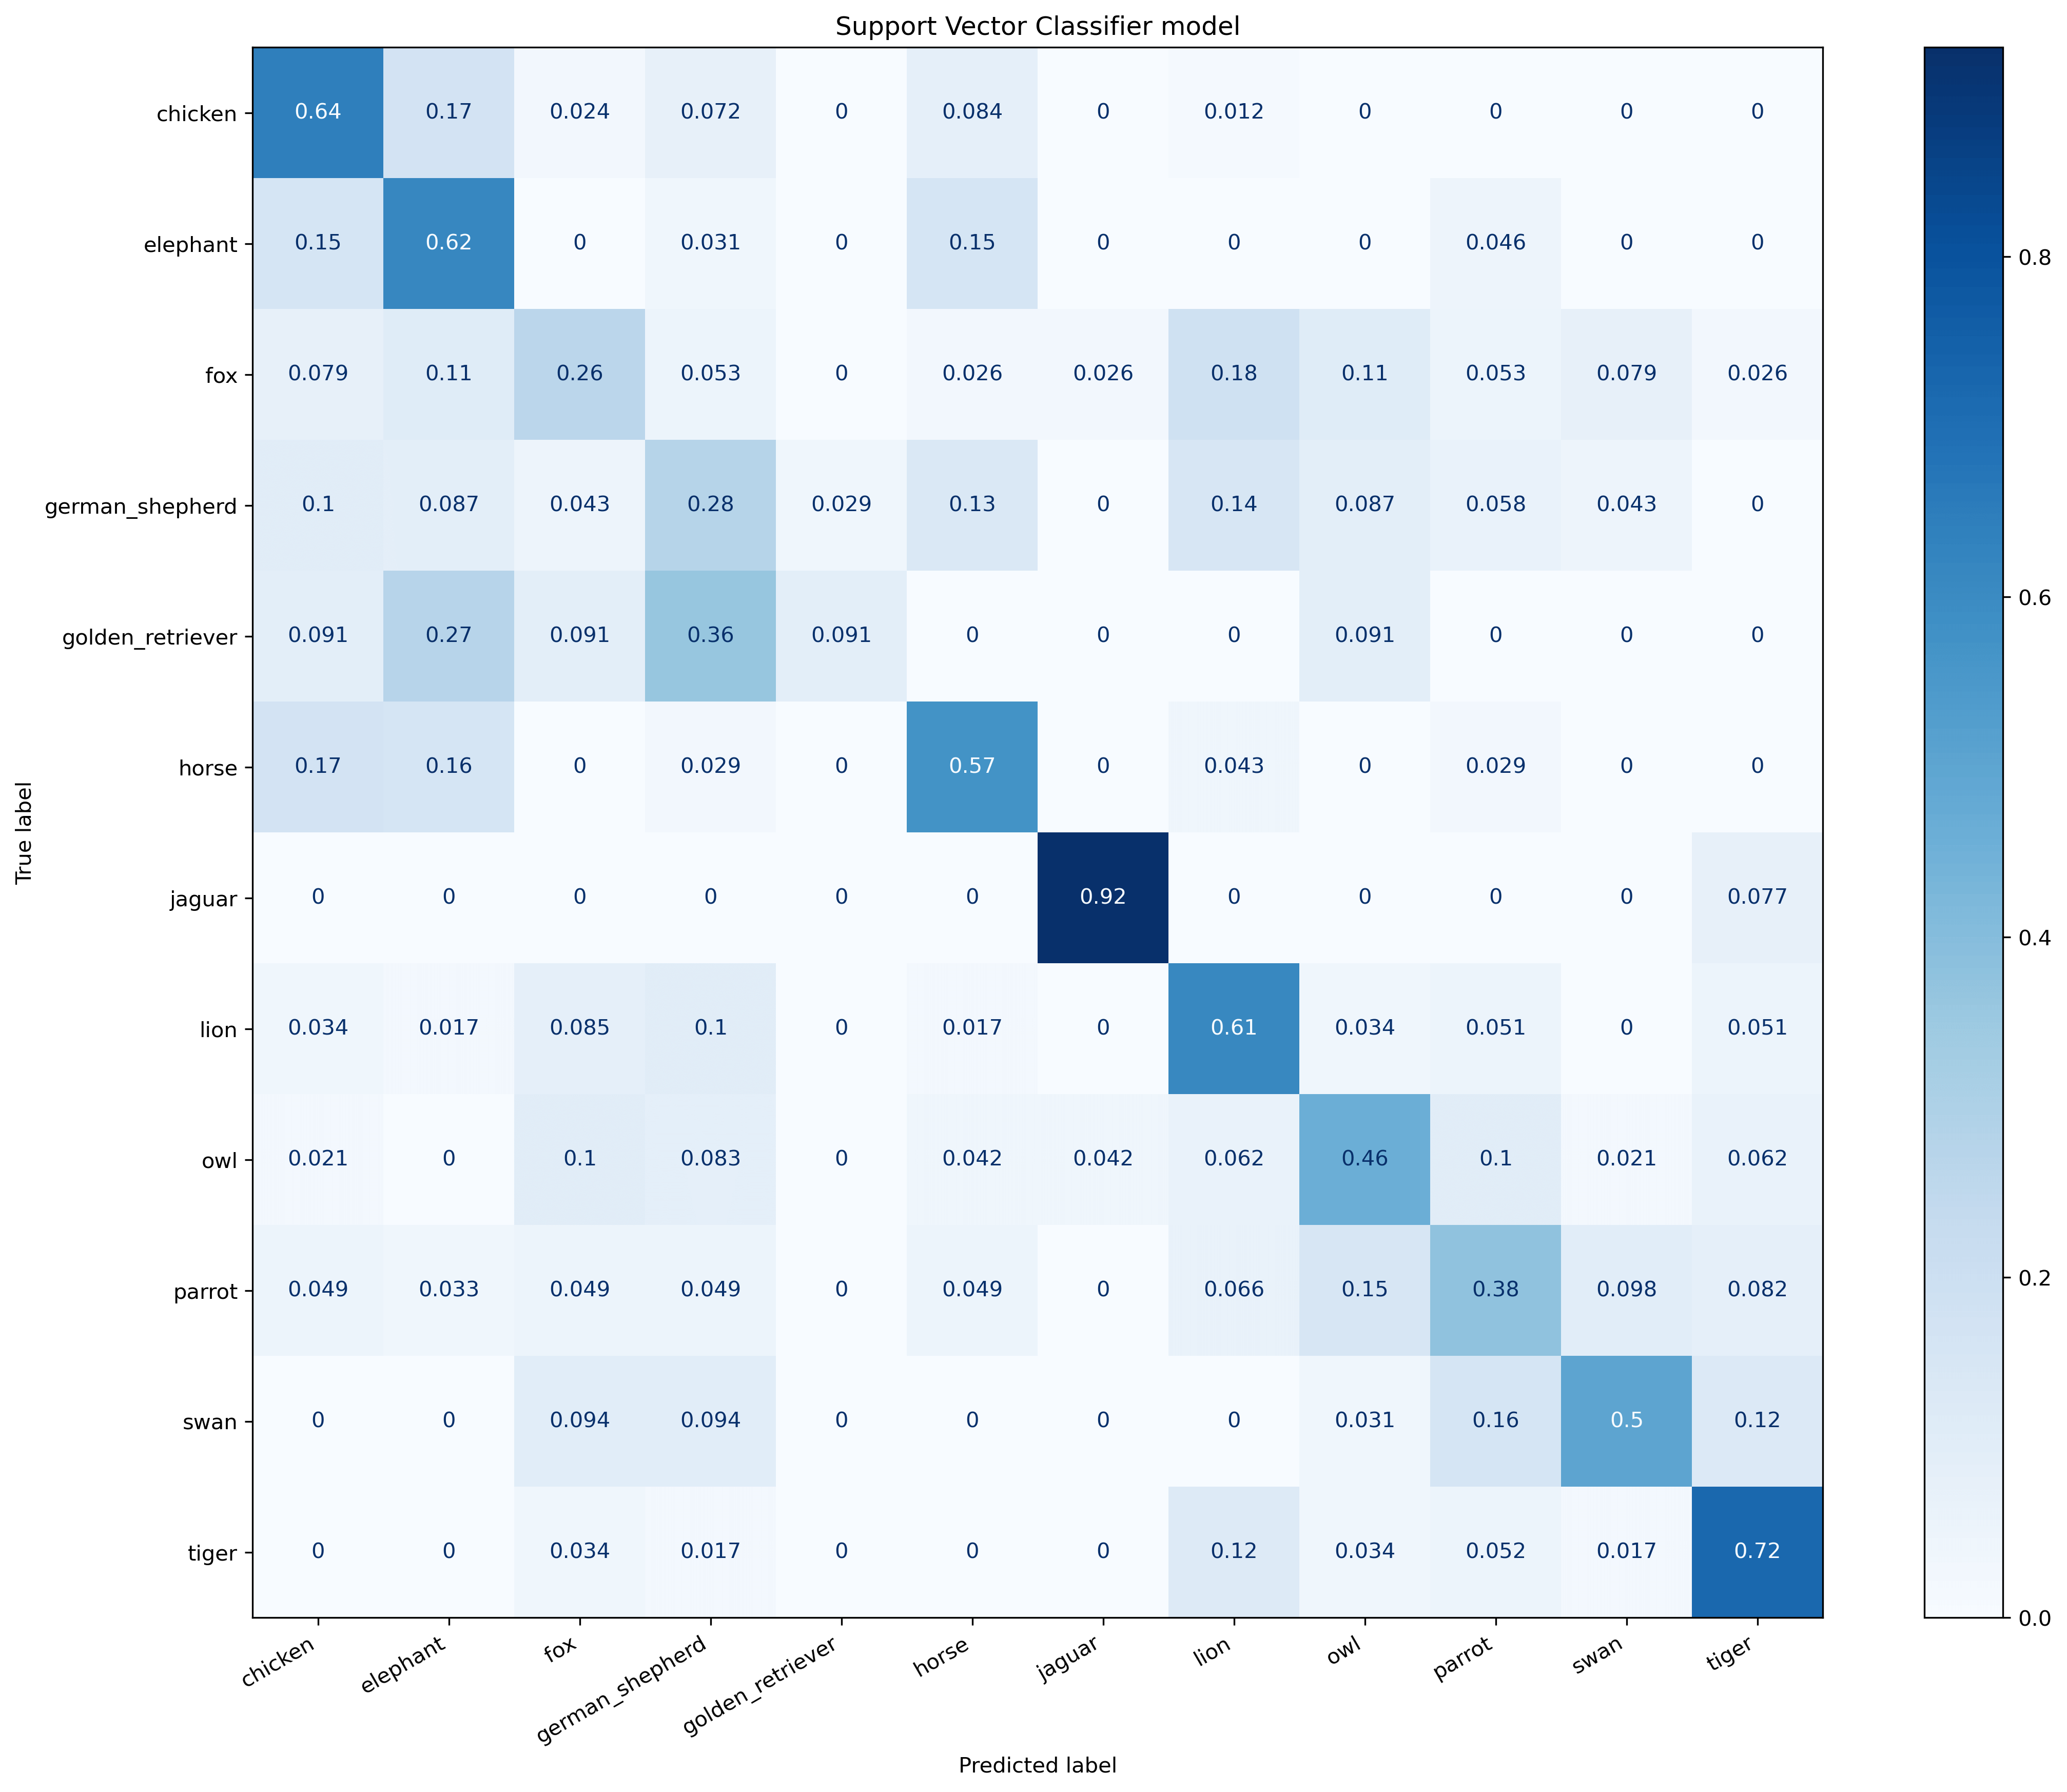
\includegraphics[width=\textwidth]{images/MA/MA_SVC_normalised.png}}
        \captionsetup{width=0.9\linewidth}
        \captionsetup{justification=centering}
        \caption{Normalised CM.}
    \end{subfigure}
    \captionsetup{width=0.8\linewidth}
    \captionsetup{justification=centering}
    \caption{Confusion matrices for the Support Vector Classifier model.}
    \label{fig:ma_svc_cm}
\end{figure*}


%------------------------------------

\section{Linear SVC and Gradient Boosting}
\label{section:ma_linSVC_grad_boost}

As discussed in part \ref{part:linear_svc}, the linear SVC variant performed worse than the just discussed SVC variant.
The confusion matrices reflect this by just performing worse overall with no noteworthy other differences.
For completeness the matrices are given in the extra's figures list (figure \ref{fig:ma_linsvc_cm}).

As discussed in part \ref{part:gradien_boost}, the Gradient Boosting model didn't perform that well.
This is also reflected in the confusion matrices, given in figure \ref{fig:ma_gb_cm}, with worse overall scores than both the SVC model and balanced LBM model.
One important thing to note is that the gradient boosting algorithm performed well on parrots compared to the other models, with an accuracy of 50\%.

\begin{figure*}[ht]
    \centering
    \begin{subfigure}{.45\textwidth}
        \centering
        \fbox{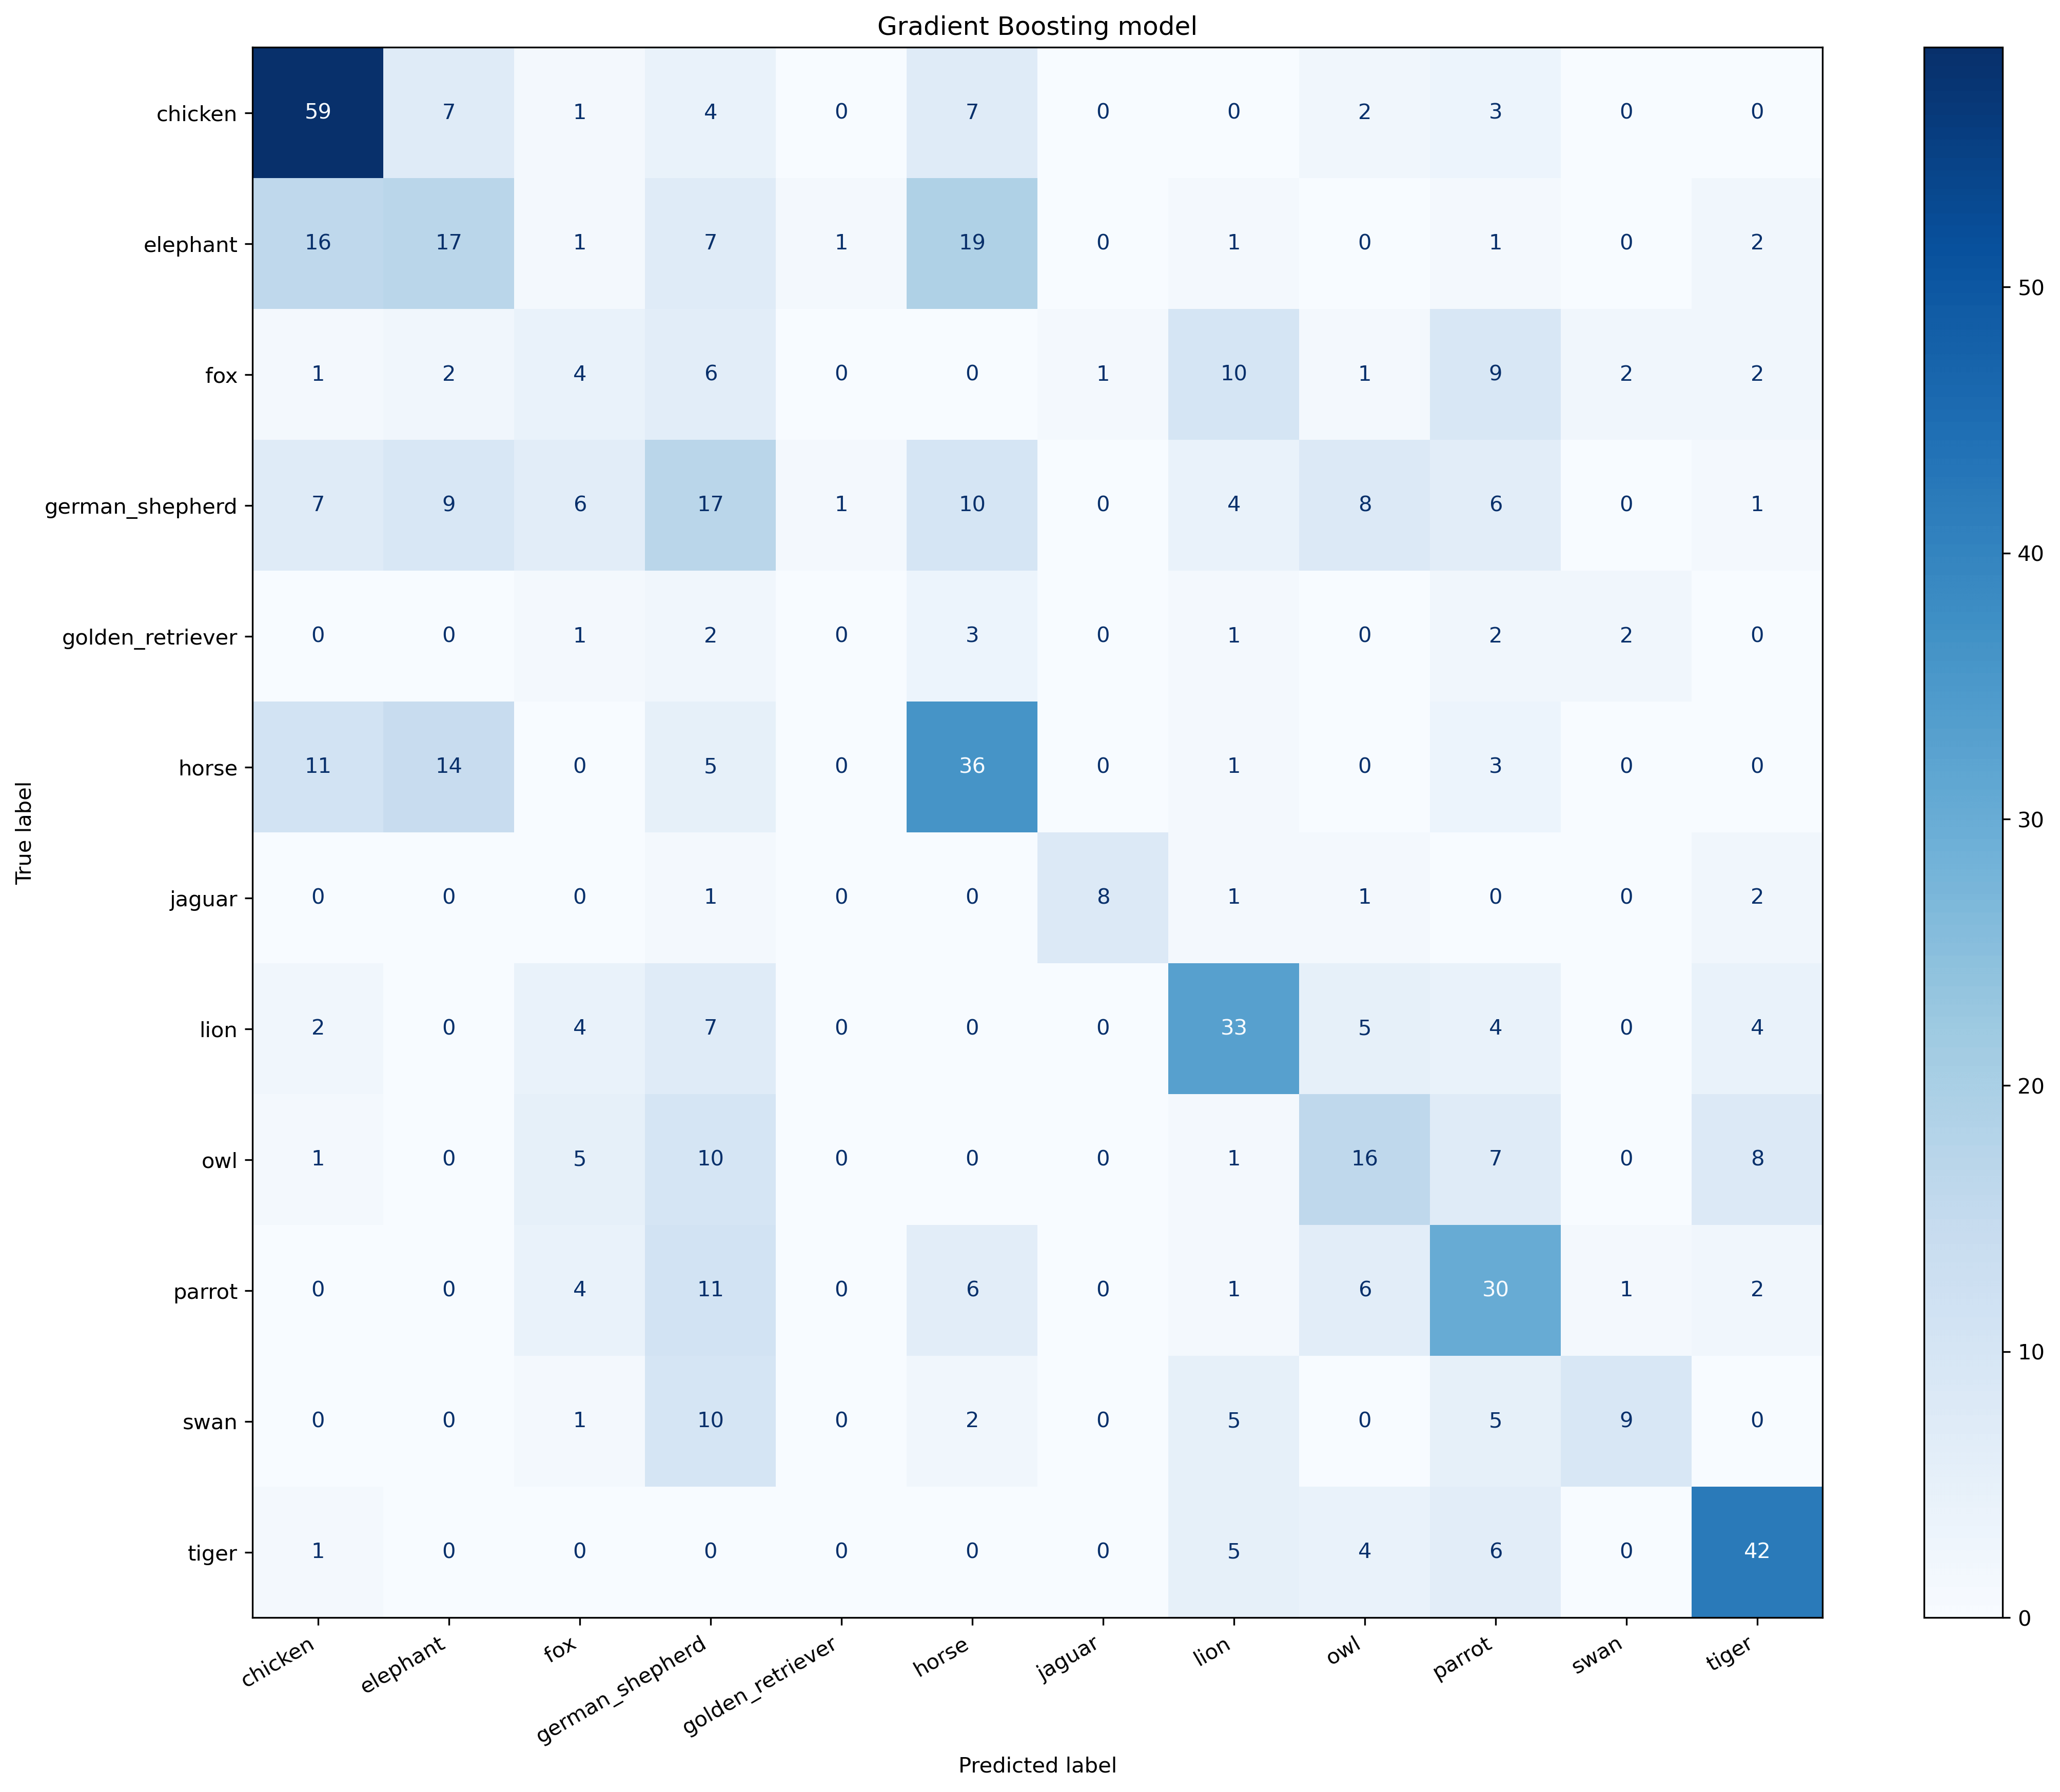
\includegraphics[width=\textwidth]{images/MA/MA_gb_non_normalised.png}}
        \captionsetup{width=0.9\linewidth}
        \captionsetup{justification=centering}
        \caption{Non normalised CM.}
    \end{subfigure}
    \hspace{1cm}
    \begin{subfigure}{.45\textwidth}
        \centering
        \fbox{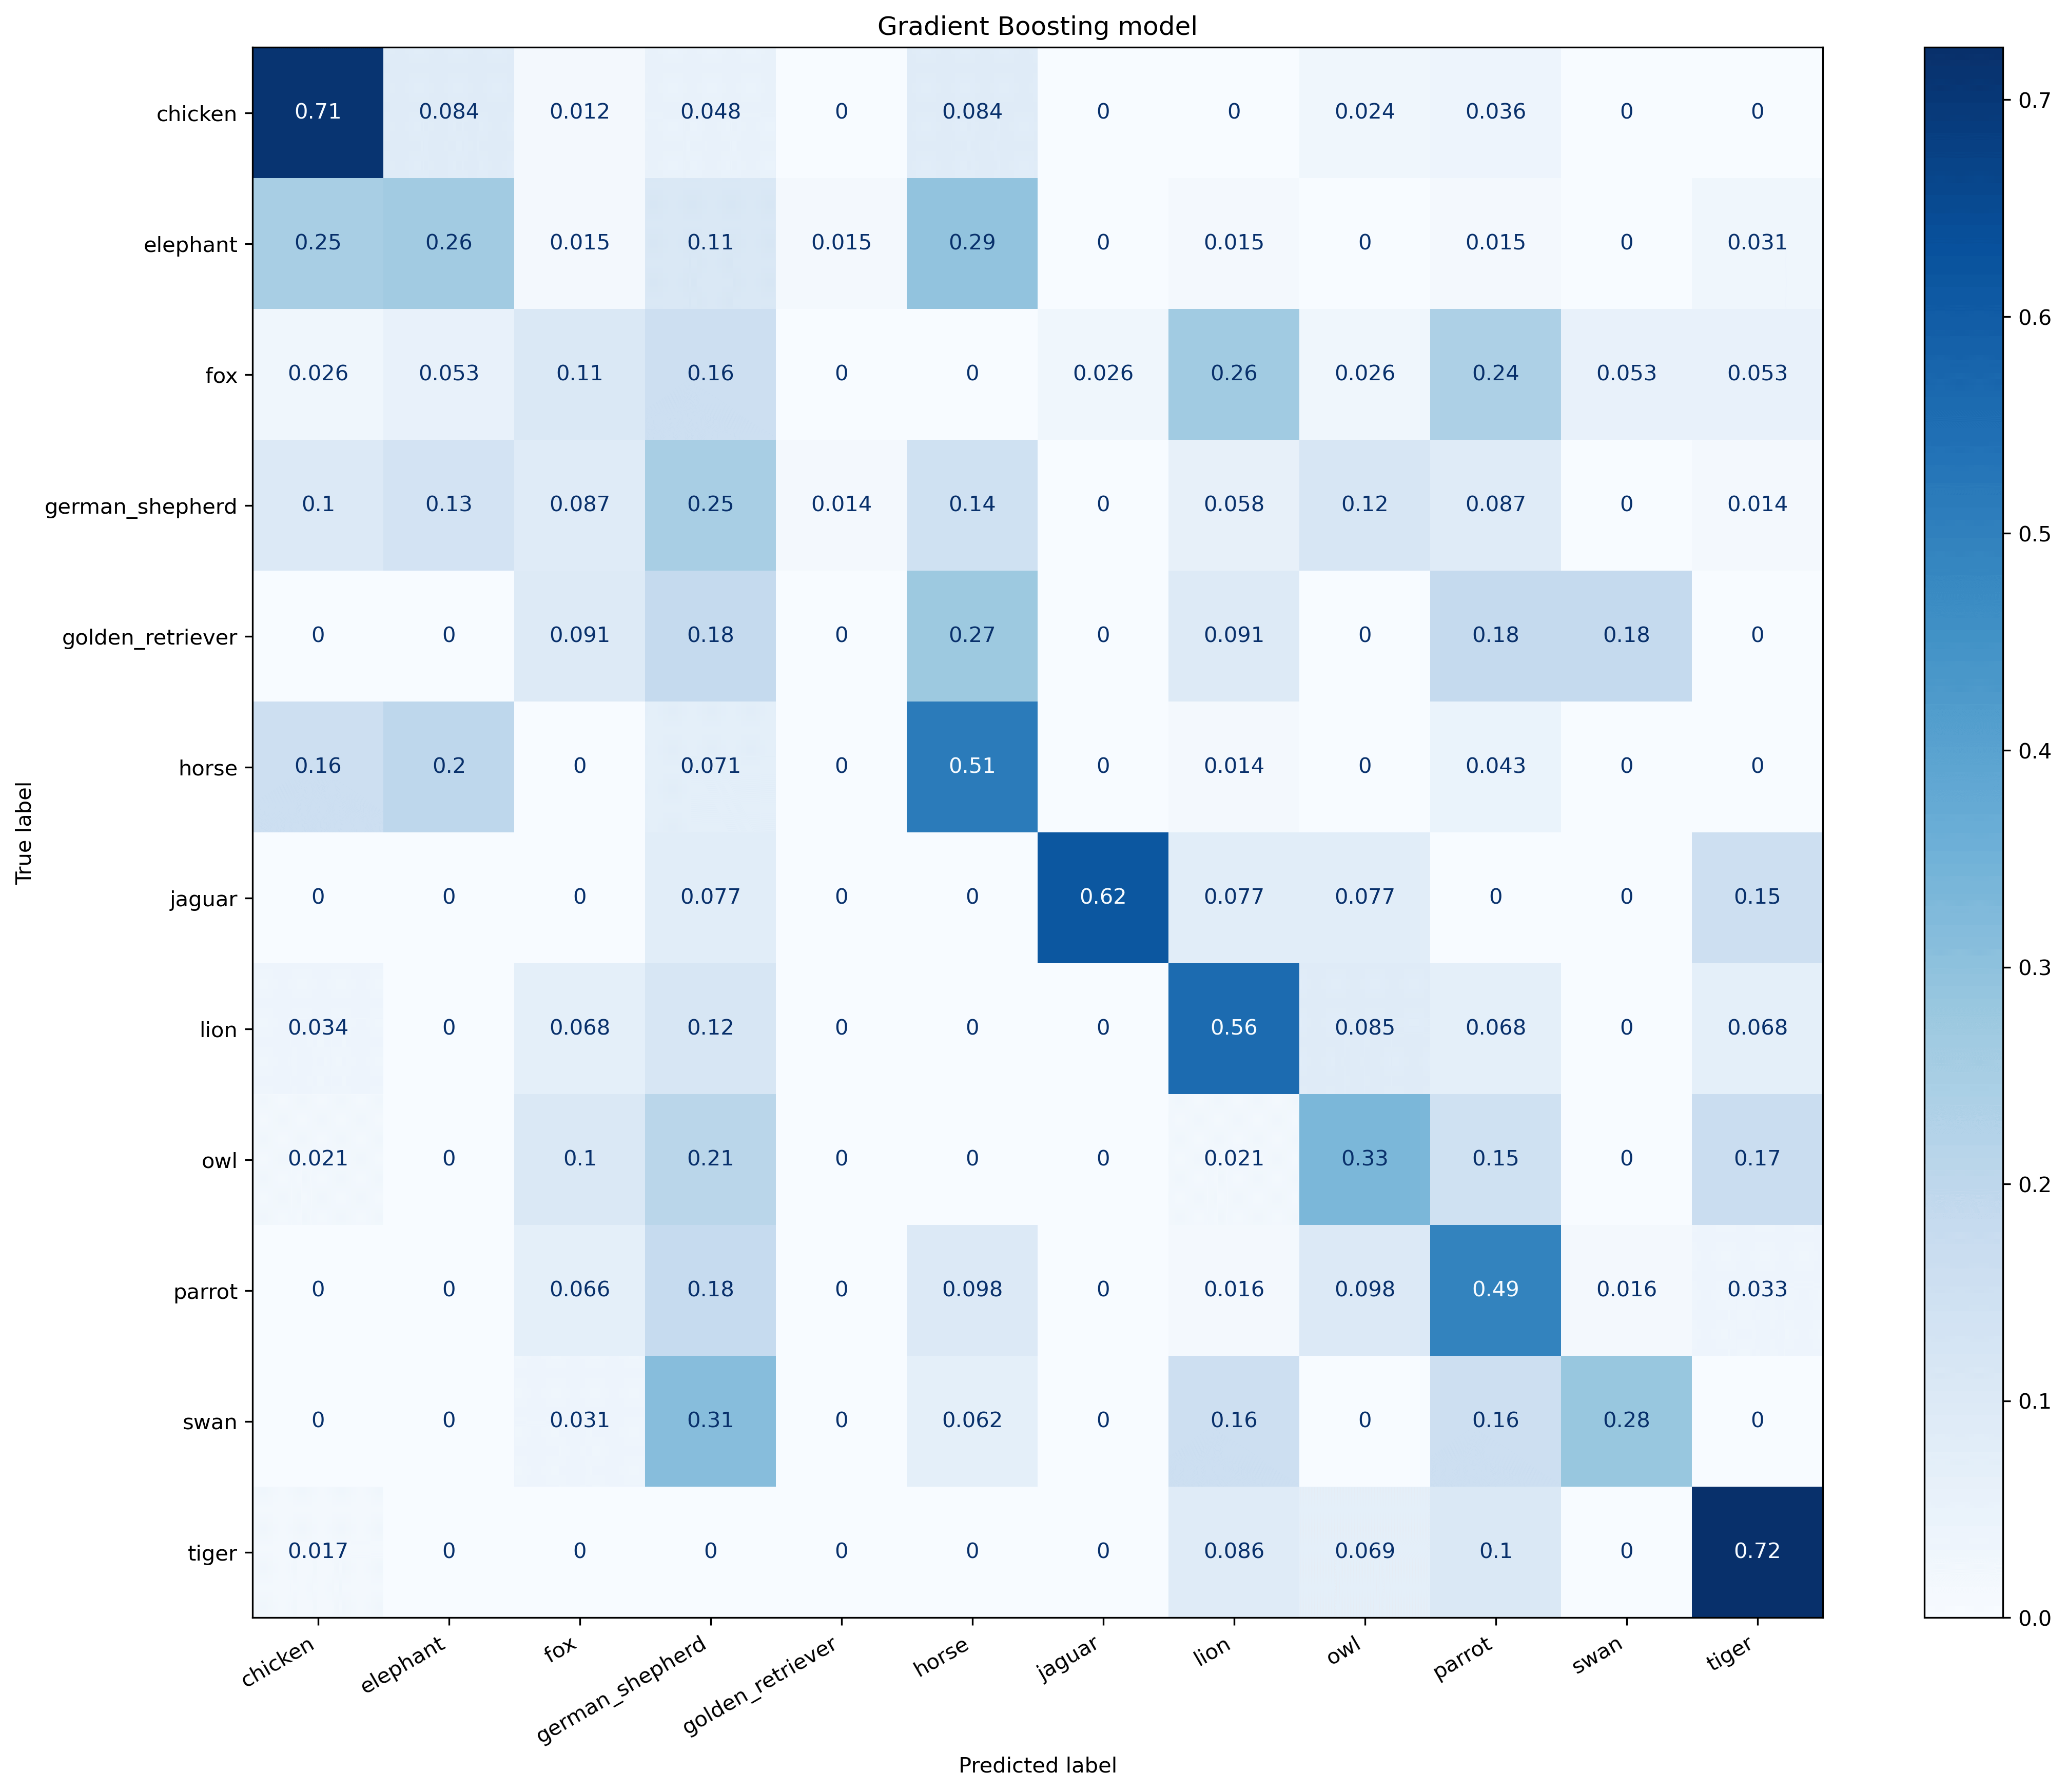
\includegraphics[width=\textwidth]{images/MA/MA_gb_normalised.png}}
        \captionsetup{width=0.9\linewidth}
        \captionsetup{justification=centering}
        \caption{Normalised CM.}
    \end{subfigure}
    \captionsetup{width=0.8\linewidth}
    \captionsetup{justification=centering}
    \caption{Confusion matrices for the Gradient Boosting model.}
    \label{fig:ma_gb_cm}
\end{figure*}

%START other optimisations
% todo CM in extra figures
\part{The final model}
\label{part:final_model}

%------------------------------------

\section{About this part}
\label{section:opt_about_part}

Whilst a great insight on the working of different models and a typical AI pipeline has been achieved with the experiments discussed so far, many things were left unexplored.
This is mostly due to limited computational power and time available.
A final attempt is made to make a better performing model using the further insight received from experiments up until now.
Things that were not tried but which are \textit{assumed} to increase performance are also listed here.
This part will only briefly discuss all steps to avoid repetition and an even longer document. 
The Notebooks corresponding with this part are \texttt{final\_model\_exploration.ipynb}, \texttt{final\_model.ipynb}, \texttt{svc\_large.ipynb},  \texttt{clustering.ipynb} and \texttt{more\_helpers.py}.
The Notebooks provide inline comments on the found results.

%------------------------------------

\section{Making a better individual model}
\label{section:opt_better_model}

Firstly, some of the made decisions early on, such as the used descriptor and cluster amount, are reconsidered.
The following things were tried to make a better performing LBM and SVC model: 
\begin{itemize}
    \item Different scalers and transformers were tried as preprocessing (after clustering). The SVC model did not benefit from this but applying the polynomial features transformer on the LBM model significantly increased the performance by 0.1 on the test set and Kaggle (now 1.57203)!
    \item The train set was balanced and overfitted, neither of which increased global or individual performance. The balanced train set does give a more representative MCLL score and thus will be used to determine the weighted probabilities for the final model.
    \item Neither \texttt{AdaBoostClassifier} or the \texttt{BaggingClassifier} to make an ensemble of the LBM and SCV models performed well. This can be expected since such ensembles work well when combining \textit{weak models}, which SVC and the LBM are not.
    \item The SIFT descriptor with 100 clusters was used as the default for this report, this is now reconsidered by testing SVC with more clusters. It was found that giving SVC more clusters drastically improved its performance without seeming to lose generality based on the confusion matrix. 1250 clusters seemed optimal.
    \item The \texttt{createCodebook} helper function uses \texttt{MiniBatchKMeans} for a given cluster amount, according to \citet{kmeansvsmini}, using this faster variant over regular K-Means results in worse performance. This was explored and it was found opting for regular K-Means does indeed increase model performance, all be it with the cost of a tremendous slower clustering. Some different clustering algorithms, such as \texttt{GaussianMixture} were also tried, but this didn't yield an increase in performance.
    \item Preprocessing after and before clustering was also considered. One of which is using \textit{RootSIFT} as proposed by \citet{rootsift}. Opting to use root-sift combined with \texttt{PowerTransformer} yielded in an even bigger increase of model performance. Special attention needs to be paid that the scaler and clustering used for the test data are the same as the one used for the training. 
\end{itemize}

%------------------------------------
%todo hieronder
\section{Combining powers}
\label{section:opt_ensemble}

Multiple models are now finalised, each having some strengths and weaknesses.
Some classes are easier to distinguish than others.
The ensembles discussed in part \ref{part:gradien_boost} suggest \textit{cleverly combining} multiple models and \textit{submodels} can increase performance, especially for the unbalanced classes.

As a final approach, a model is made which uses multiple models and submodels under the hood.
This final model is represented by the custom class \texttt{FinalModel} which has a \texttt{fit}, \texttt{predict} and a \texttt{predict\_proba} function.
Since this isn't a scikit classifier, another way of generating confusion matrices is considered by editing open-source code by \citet{pretty_cm}.
The weight given to certain classifiers is determined from their confusion matrix.
All of the confusion matrices for the underlying models are given in the extra figures list.
The general flow of the final model is as follows:

\begin{itemize}
    \item When fitting the model, multiple underlying models are fitted. These models are:
    \begin{itemize}
        \item The Linear Baseline Model (LBM) and Support Vector Classifier (SVC) for all of the input data.
        \item The LBM and SVC model to distinguish between 5 merged classes based on similarity from mislabelling:
        \begin{itemize}
            \item Chicken.
            \item Big: horse and elephant.
            \item Catish: fox, lion, tiger and jaguar.
            \item Dog: German shepherd and golden retriever.
            \item Flying: owl, parrot and swan.
        \end{itemize}
        \item The LBM and SVC to distinguish between \textit{dogs or others}.
        \item The LBM and SVC sub-model for classifying a subset:
        \begin{itemize}
            \item Big: horse and elephant.
            \item Catish: fox, lion, tiger and jaguar.
            \item Dog: German shepherd and golden retriever.
            \item Flying: owl, parrot and swan.
        \end{itemize}
    \end{itemize}
    \item When predicting proabilities, the following steps occur:
    \begin{itemize}
        \item The \texttt{predict\_proba} function for all underlying models is called and the results are saved.
        \item The final probabilities to return is determined as follows:
        \clearpage
        \begin{itemize}
            \item If the SVC or LBM model's \texttt{predict\_proba} is very certain, 96\%+ and 98\%+ respectively, it's probabilities are returned.
            \item If SVC or LBM model for distinguishing the merged classes:
            \begin{itemize}
                \item Is very certain (92\% to 95\%+), then
                \item The scores received from the related sub-models are added to the scores for all animals, then
                \item The resulting probabilities are renormalized, thus
                \item The animals from the merged class have \textit{boosted} probabilities (by a factor of 4)
            \end{itemize}
            \item If SVC or LBM model for distinguishing the merged classes:
            \begin{itemize}
                \item Is somewhat certain (82\% to 86\%+), then
                \item The scores received from the related sub-models are added to the scores for all animals, then
                \item The resulting probabilities are renormalized, thus
                \item The animals from the merged class have \textit{boosted} probabilities (by a factor of 0.5)
            \end{itemize}
            \item If all of the above didn't yield a result, the classifier (SVC or LBM) that has the highest certainty after weighing with accuracy, is chosen.
        \end{itemize}
    \end{itemize}
\end{itemize}

%------------------------------------

\section{Unexplored possibilities}
\label{section:opt_unexplored}

Whilst the achieved model performance is above average when looking at the Kaggle leader board, some interesting possible optimisations that came to mind could improve it even more.
To show that these were thought of and as possible further extensions some unexplored possibilities are listed here:
\begin{itemize}
    \item Fine-tuning and preprocessing the SIFT descriptor, although trivial actions such as resizing are expected to have minimal impact since SIFT determines interesting points in a manner which is not directly dependent on orientation or size.
    \item Perhaps making a selection of the found features and clusters might further aid performance. For example: Using the correlation matrix to remove disruptive features or clusters.
    \item Using a different descriptor such as HoG (Histogram of Gradients) which is said to work well with humans and animals.
    \item Trying more models such as XGBoost, a modification on the tried Gradient Boosting model said to work well with animals.
    \item Only the LBM model was explored with different descriptors and cluster amounts. The SVC model with rbf kernel was also tested with varying cluster amounts. Ideally, all models should be tested with all descriptors and varying cluster amounts, but this is (very!) time-consuming and increasing cluster amounts increases the risk of overfitting.
    \item The parameters for the sub-models could be further fine-tuned.
\end{itemize}

%------------------------------------
\clearpage
\section{The final models and received score}
\label{section:opt_score}

The two models that will be submitted for the Kaggle submission are the best performing SVC model and the final model discussed in this part.
These models differ quite a lot when looking at the confusion matrices given in figure \ref{fig:final_model_cm}.
The SVC model reaches higher peaks when looking at the best performance on a certain class while the final model seems more balanced.
The Kaggle score of the best SVC model is 1.35777, the score of the best final model is 1.40394. 
This again suggests the data for the public leaderboard isn't that balanced.

\begin{figure*}[ht]
    \centering
    \begin{subfigure}{.45\textwidth}
        \centering
        \fbox{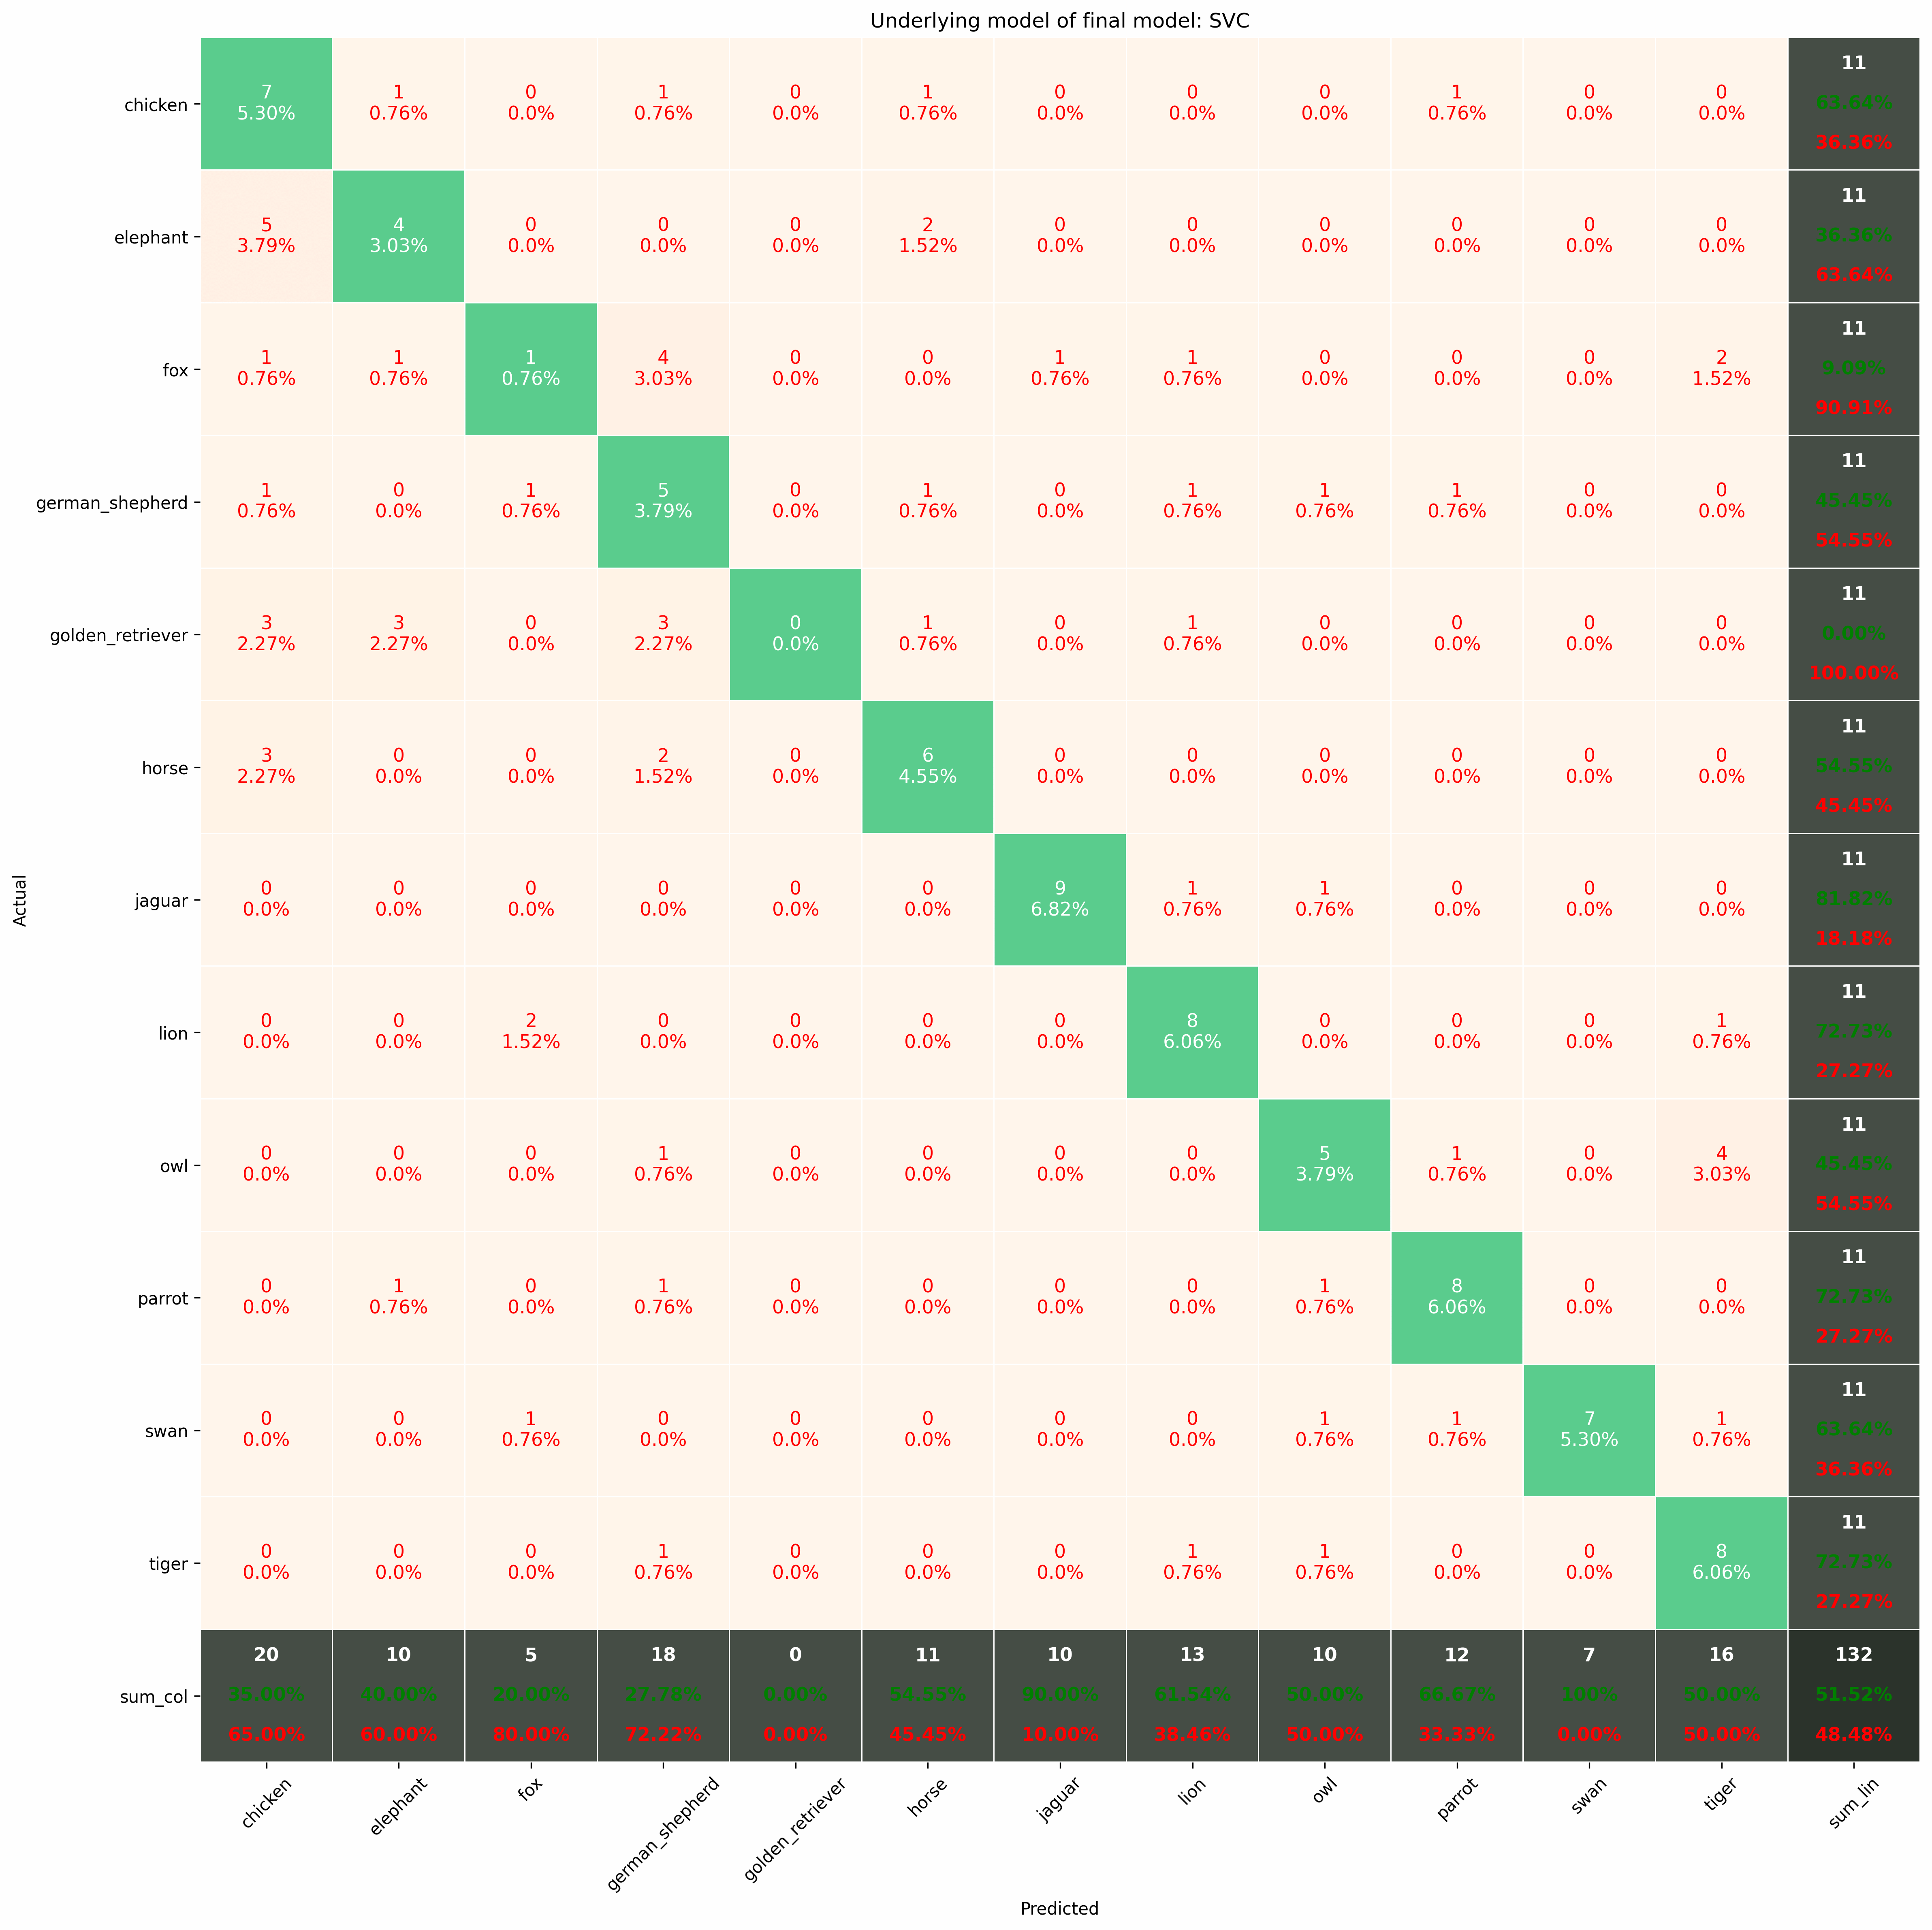
\includegraphics[width=\textwidth]{images/final/underlying_SVC.png}}
        \captionsetup{width=0.9\linewidth}
        \captionsetup{justification=centering}
        \caption{CM of the final model's underlying SVC model.}
    \end{subfigure}
    \hspace{1cm}
    \begin{subfigure}{.45\textwidth}
        \centering
        \fbox{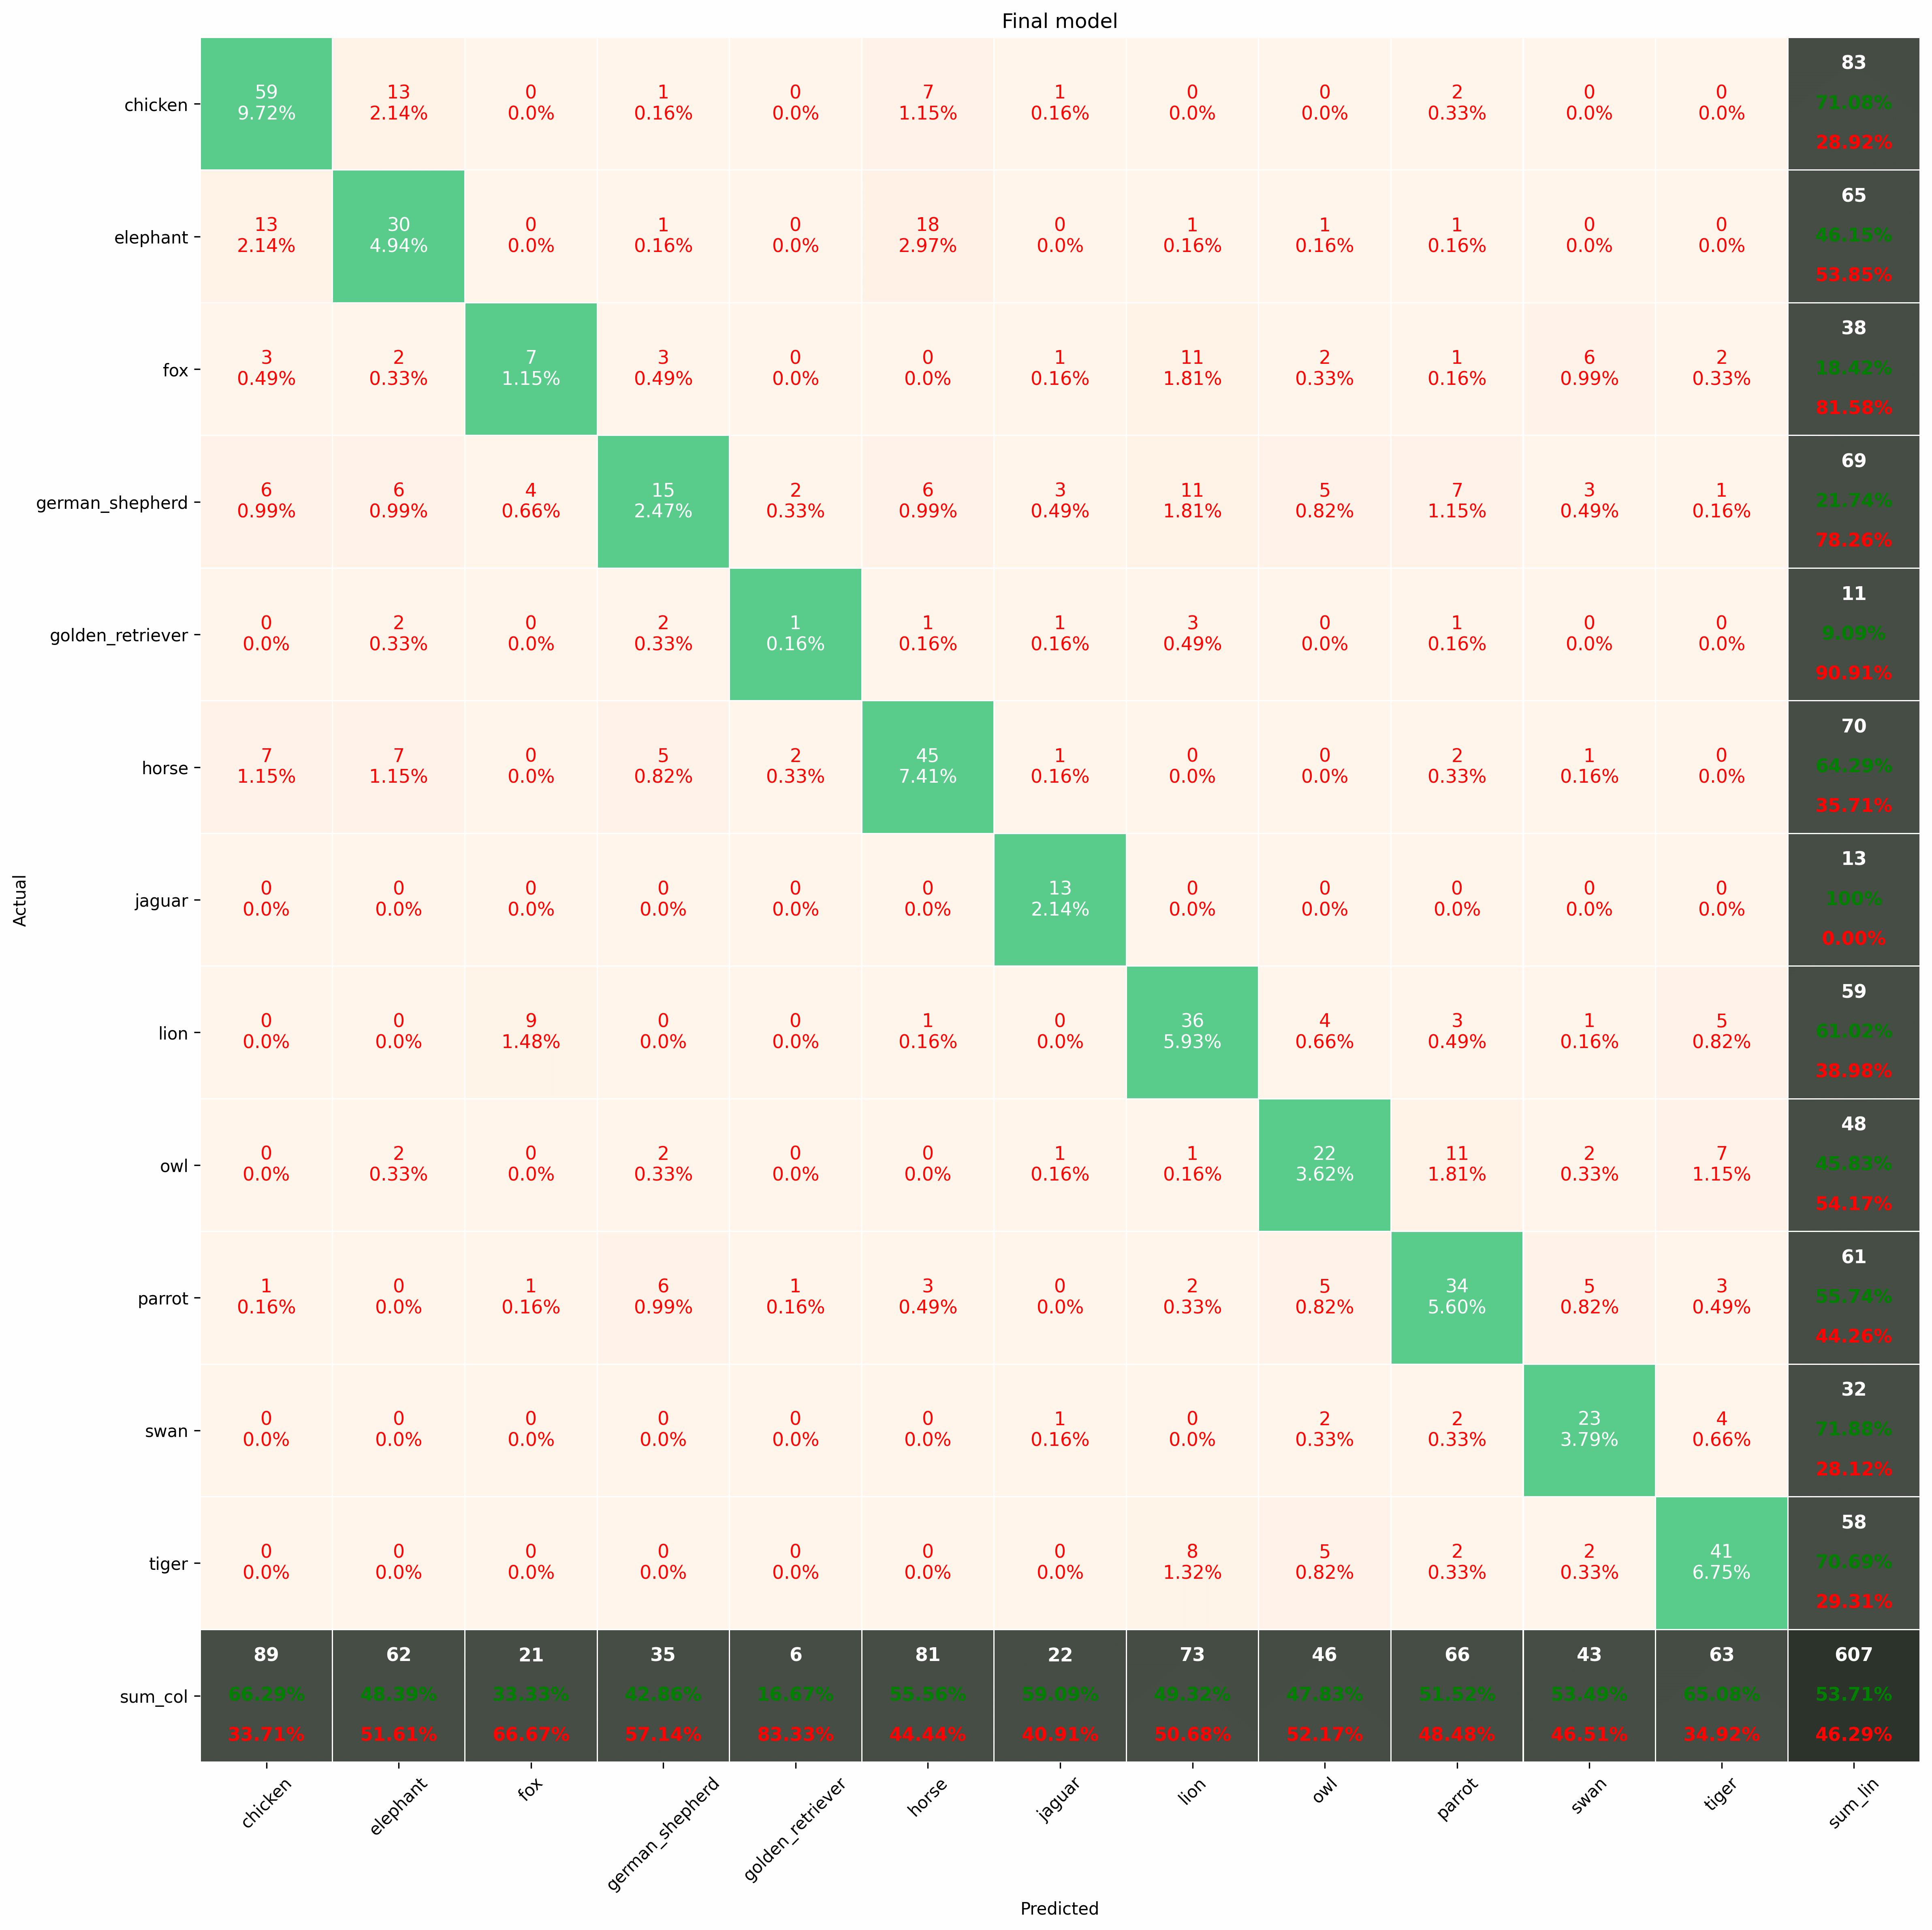
\includegraphics[width=\textwidth]{images/final/final_cm.png}}
        \captionsetup{width=0.9\linewidth}
        \captionsetup{justification=centering}
        \caption{CM of the final model.}
    \end{subfigure}
    \captionsetup{width=0.8\linewidth}
    \captionsetup{justification=centering}
    \caption{Confusion matrices of the final model and its underlying SVC model.}
    \label{fig:final_model_cm}
\end{figure*}

%START conclusion
% TODO volledig
\part{Conclusion}
\label{part:conclusion}

%------------------------------------

\section{What is learned}
\label{section:con_achieved}

TODO XXX

%------------------------------------

\section{The hurdles}
\label{section:con_hurdles}

TODO XXX

%------------------------------------

\section{Further extensions}
\label{section:con_extensions}

TODO XXX

%START figures
\chapter*{More figures}
\addcontentsline{toc}{chapter}{More figures}

Some figures are referred to in the text but not placed directly under the text. These are included in this list. All figures are high resolution thus zooming in the PDF should be viable to get a clearer view.

%------------------------------------

\section*{Overview of training set}

\begin{figure}[H]
    \begin{center}
        \fbox{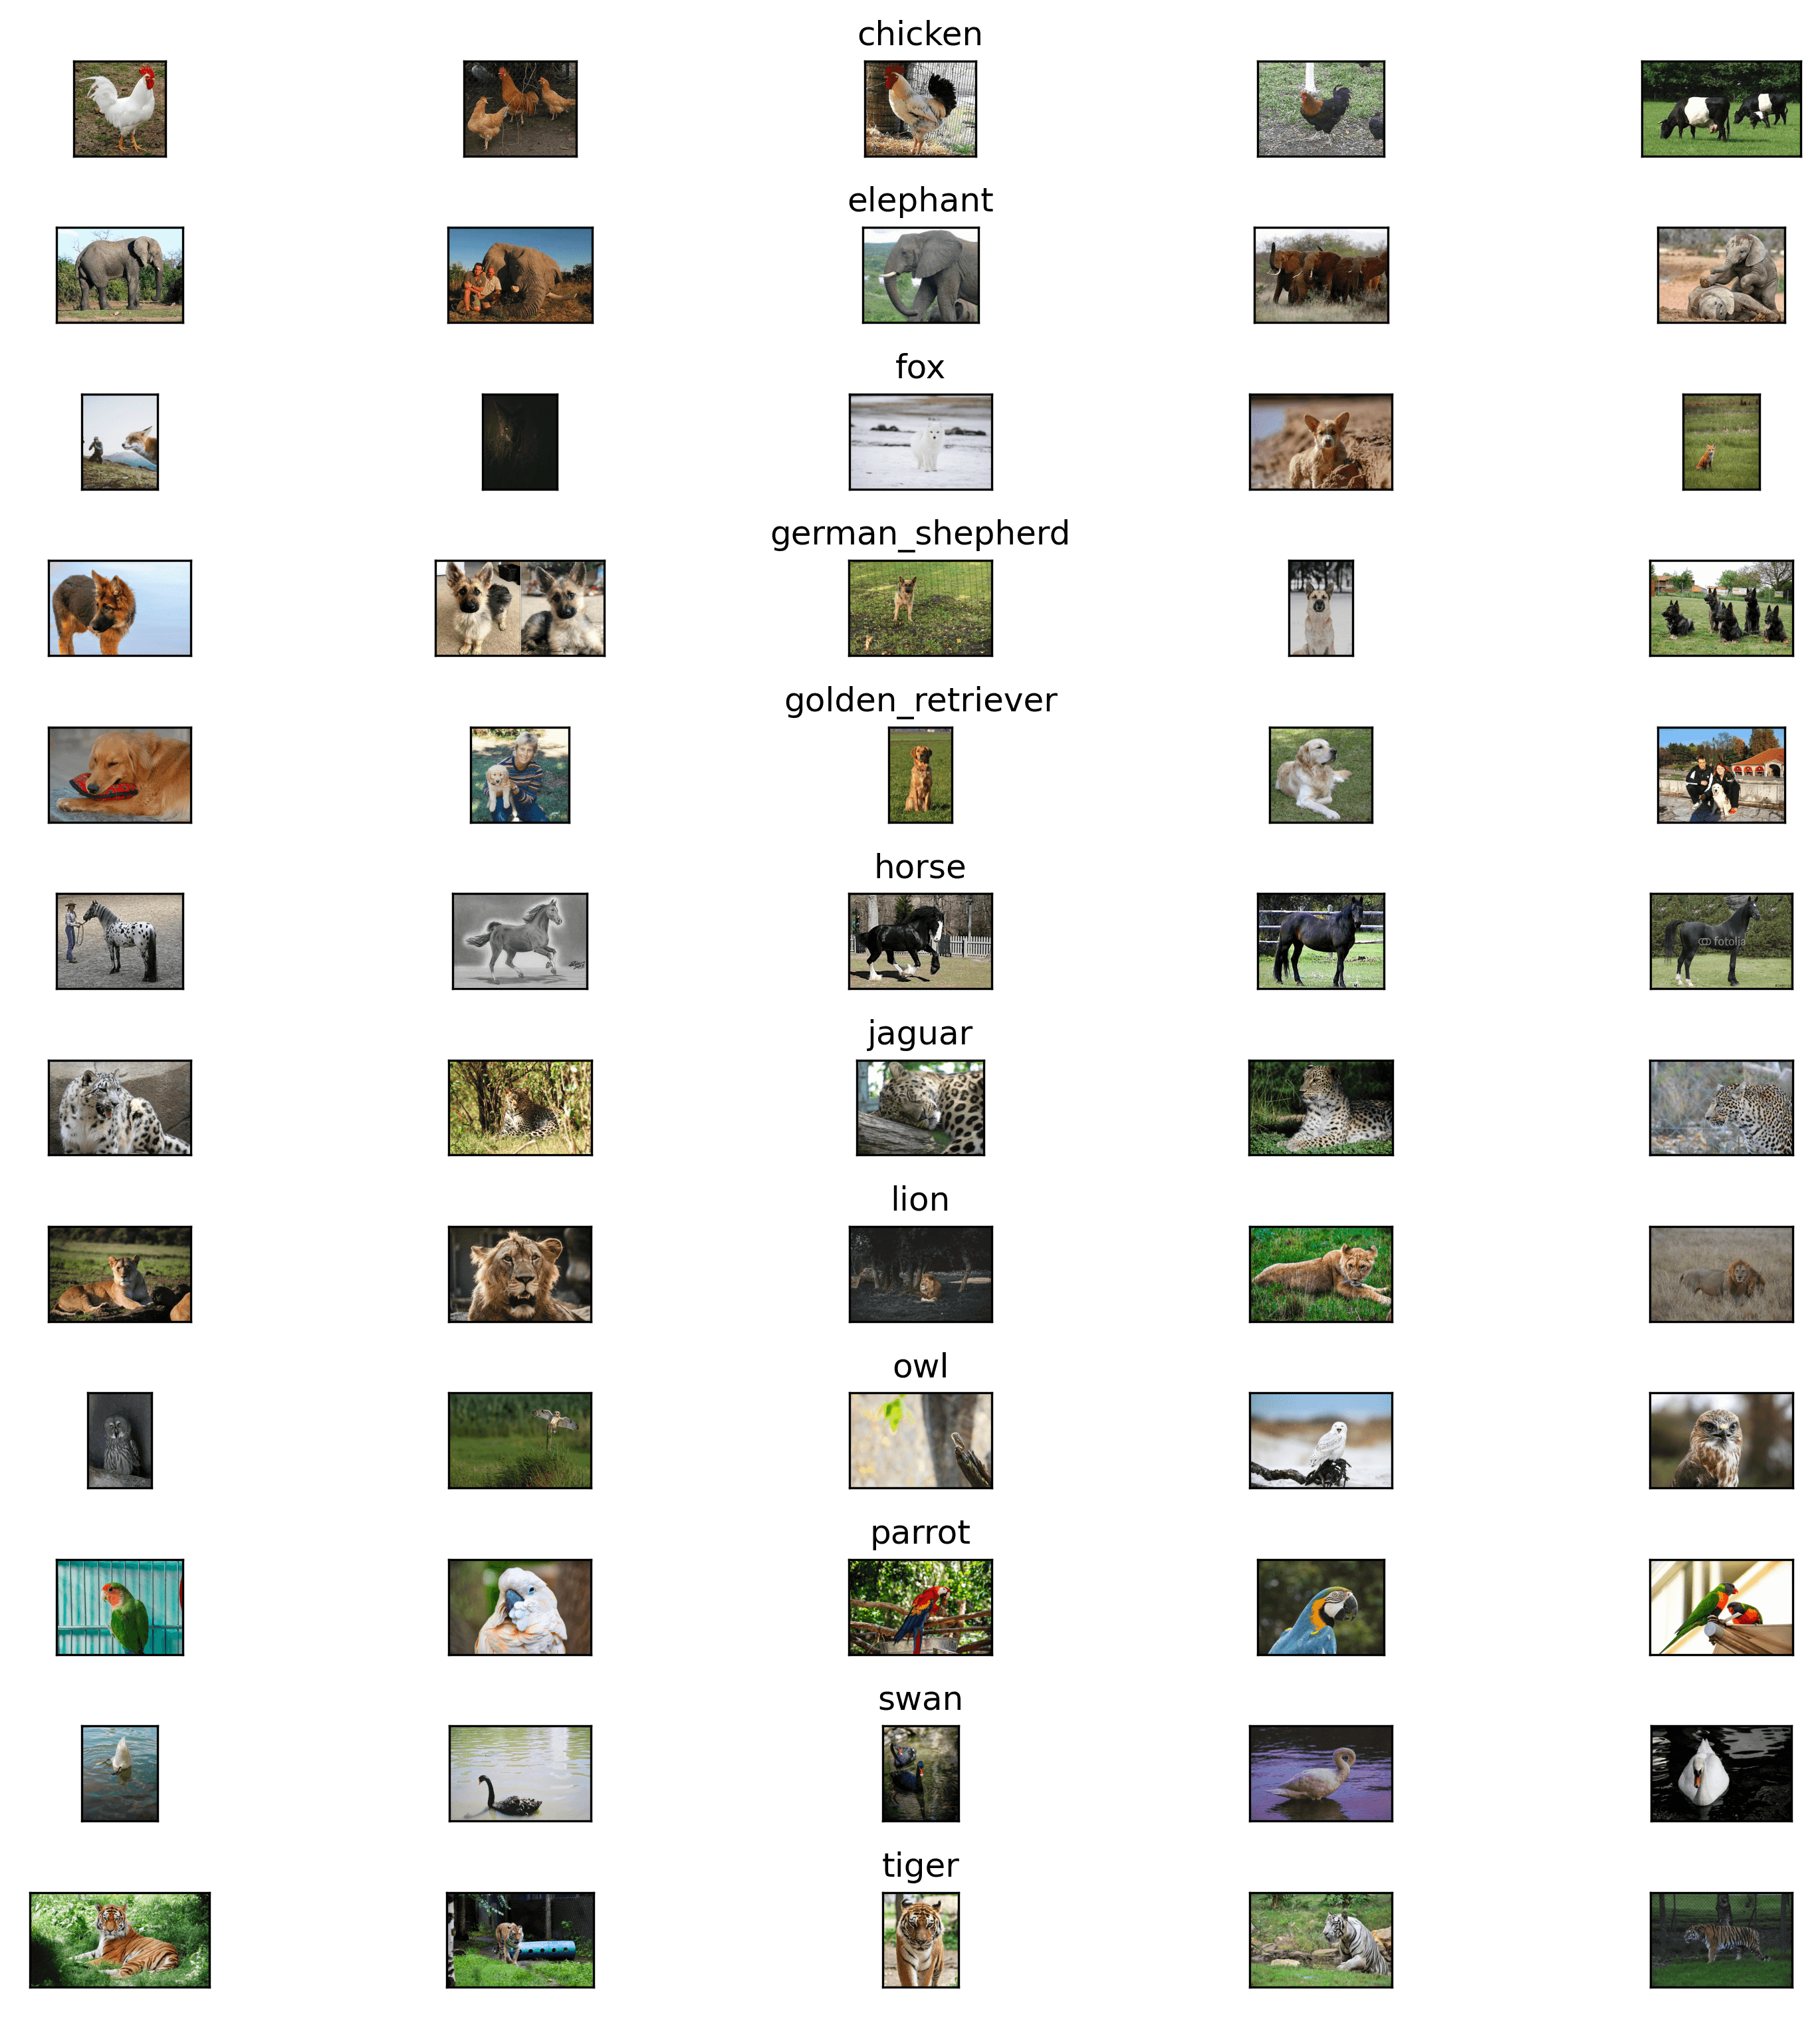
\includegraphics[width=0.70\linewidth]{images/1-data_analysis-labeled_data_overview.png}}
    \end{center}
    \captionsetup{width=0.65\linewidth}
    \captionsetup{justification=centering}
    \caption{An overview of the supplied data per class.}
    \label{fig:1-data_analysis-labeled_data_overview.png}
\end{figure}

%------------------------------------

\section*{Overview of features data}

\begin{figure}[H]
    \fbox{\includegraphics[width=1\linewidth]{images/1-data_analysis-feature_representation.png}}
    \captionsetup{width=0.85\linewidth}
    \captionsetup{justification=centering}
    \caption{An overview of the first 30 features data from a SIFT descriptor.}
    \label{fig:1-data_analysis-feature_representation}
\end{figure}

%------------------------------------

\section*{Linear baseline model - input optimisation (small)}

\begin{figure}[H]
  \centering
  \begin{minipage}[b]{0.4\textwidth}
    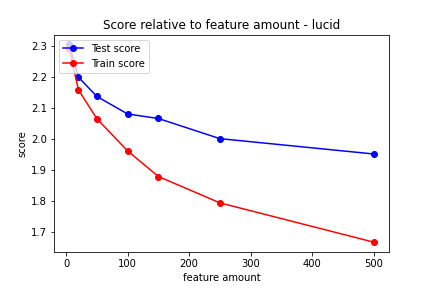
\includegraphics[width=\textwidth]{images/2-LBM-feature_amount_lucid_small_values.png}
  \end{minipage}
  \hfill
  \begin{minipage}[b]{0.4\textwidth}
    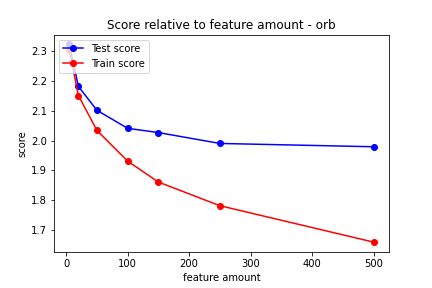
\includegraphics[width=\textwidth]{images/2-LBM-feature_amount_orb_small_values.png}
  \end{minipage}
\end{figure}

\begin{figure}[H]
  \centering
  \begin{minipage}[b]{0.4\textwidth}
    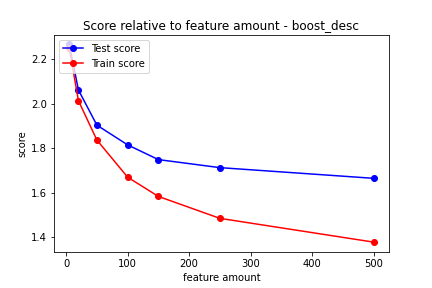
\includegraphics[width=\textwidth]{images/2-LBM-feature_amount_boost_desc_small_values.png}
  \end{minipage}
  \hfill
  \begin{minipage}[b]{0.4\textwidth}
    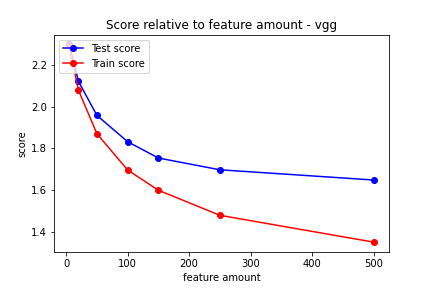
\includegraphics[width=\textwidth]{images/2-LBM-feature_amount_vgg_small_values.png}
  \end{minipage}
\end{figure}

\begin{figure}[H]
  \centering
  \begin{minipage}[b]{0.4\textwidth}
    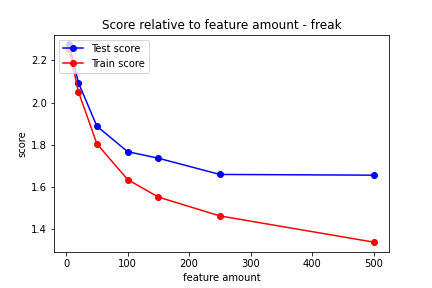
\includegraphics[width=\textwidth]{images/2-LBM-feature_amount_freak_small_values.png}
  \end{minipage}
  \hfill
  \begin{minipage}[b]{0.4\textwidth}
    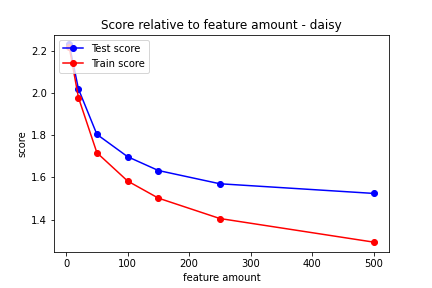
\includegraphics[width=\textwidth]{images/2-LBM-feature_amount_daisy_small_values.png}
  \end{minipage}
\end{figure}

\begin{figure}[H]
  \centering
  \begin{minipage}[b]{0.4\textwidth}
    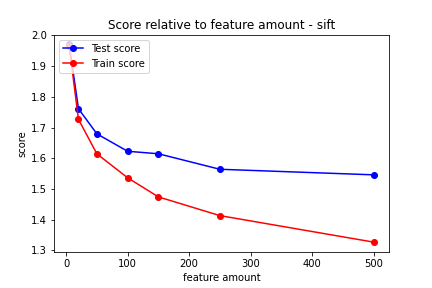
\includegraphics[width=\textwidth]{images/2-LBM-feature_amount_sift_small_values.png}
  \end{minipage}
\end{figure}

%------------------------------------

\section*{Linear baseline model - input optimisation (large)}

\begin{figure}[H]
  \centering
  \begin{minipage}[b]{0.4\textwidth}
    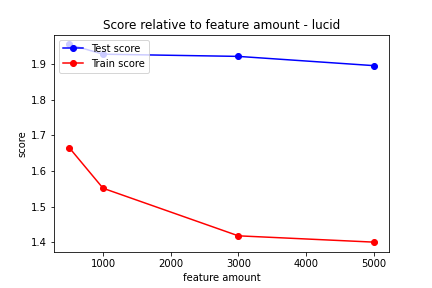
\includegraphics[width=\textwidth]{images/2-LBM-feature_amount_lucid_large_values.png}
  \end{minipage}
  \hfill
  \begin{minipage}[b]{0.4\textwidth}
    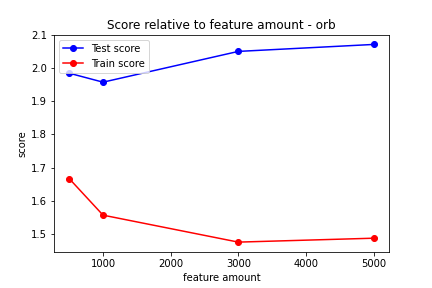
\includegraphics[width=\textwidth]{images/2-LBM-feature_amount_orb_large_values.png}
  \end{minipage}
\end{figure}

\begin{figure}[H]
  \centering
  \begin{minipage}[b]{0.4\textwidth}
    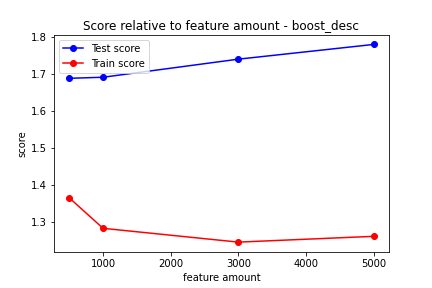
\includegraphics[width=\textwidth]{images/2-LBM-feature_amount_boost_desc_large_values.png}
  \end{minipage}
  \hfill
  \begin{minipage}[b]{0.4\textwidth}
    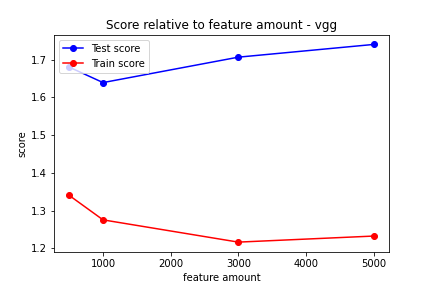
\includegraphics[width=\textwidth]{images/2-LBM-feature_amount_vgg_large_values.png}
  \end{minipage}
\end{figure}

\begin{figure}[H]
  \centering
  \begin{minipage}[b]{0.4\textwidth}
    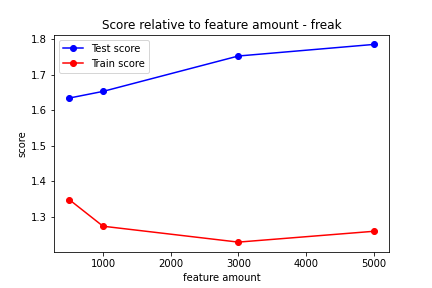
\includegraphics[width=\textwidth]{images/2-LBM-feature_amount_freak_large_values.png}
  \end{minipage}
  \hfill
  \begin{minipage}[b]{0.4\textwidth}
    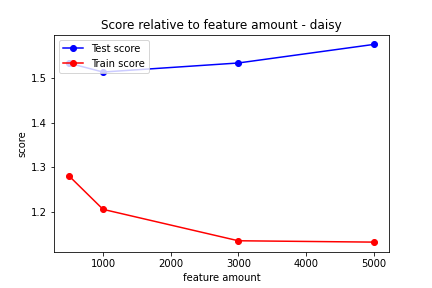
\includegraphics[width=\textwidth]{images/2-LBM-feature_amount_daisy_large_values.png}
  \end{minipage}
\end{figure}

\begin{figure}[H]
  \centering
  \begin{minipage}[b]{0.4\textwidth}
    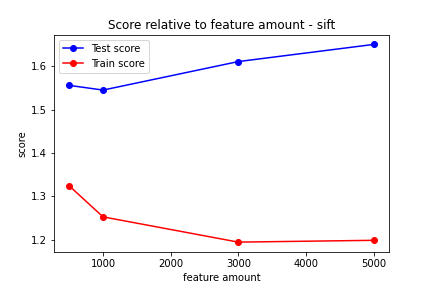
\includegraphics[width=\textwidth]{images/2-LBM-feature_amount_sift_large_values.png}
  \end{minipage}
\end{figure}

%------------------------------------

\section*{Linear baseline model - optimal DAISY}

\begin{figure}[H]
    \fbox{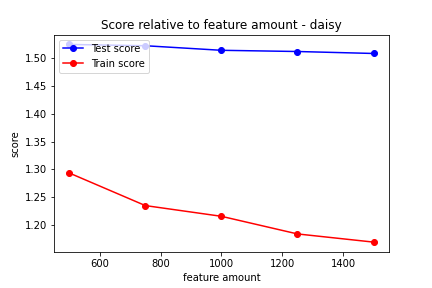
\includegraphics[width=1\linewidth]{images/2-LBM-feature_amount_daisy_daisy_optimal.png}}
    \captionsetup{width=0.85\linewidth}
    \captionsetup{justification=centering}
    \caption{An extra test for finding the optimal feature amounts for the DAISY descriptor.}
    \label{fig:2-LBM-feature_amount_daisy_daisy_optimal}
\end{figure}

%------------------------------------

\section*{Linear baseline model - class weight parameter}

\begin{figure}[H]
    \fbox{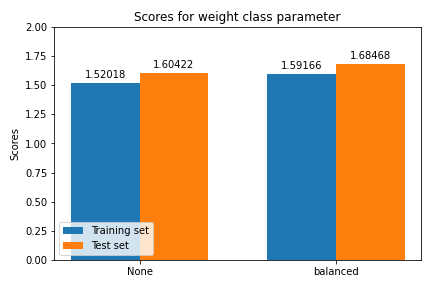
\includegraphics[width=1\linewidth]{images/2-LBM-model_weight_class.png}}
    \captionsetup{width=0.85\linewidth}
    \captionsetup{justification=centering}
    \caption{Average multi-class Log Loss score over 10 iterations.}
    \label{fig:2-LBM-model_weight_class}
\end{figure}

%------------------------------------

\section*{Linear baseline model - fit intercept parameter}

\begin{figure}[H]
    \fbox{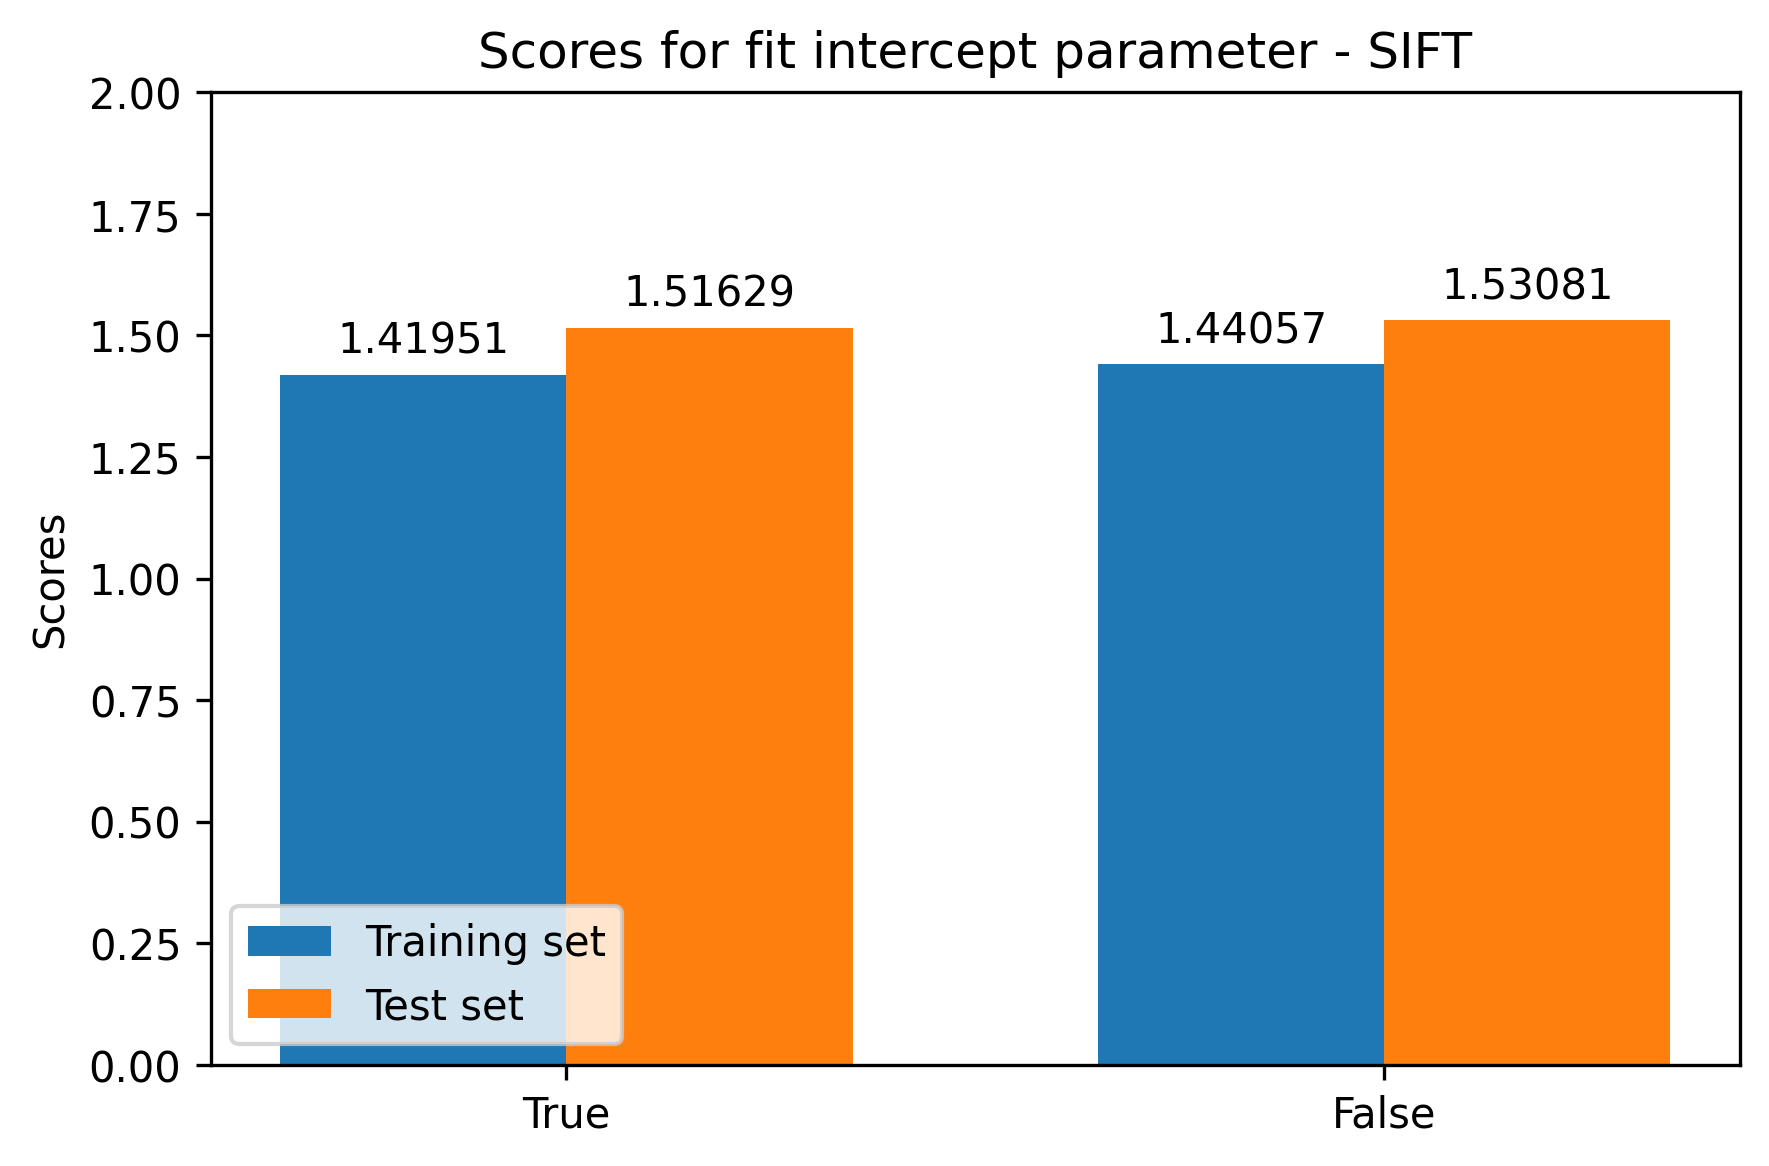
\includegraphics[width=1\linewidth]{images/2-LBM-model_fit_intercept.png}}
    \captionsetup{width=0.85\linewidth}
    \captionsetup{justification=centering}
    \caption{Average multi-class Log Loss score over 5 iterations.}
    \label{fig:2-LBM-model_fit_intercept}
\end{figure}

%references list
\nocite{*}
\printbibliography[heading=bibintoc, title={References}]

%START appendix
\chapter*{Appendix A: Working and representation of the descriptors}
\addcontentsline{toc}{chapter}{Appendix A: Working and representation of the descriptors}

\section*{Feature extraction}

Some feature extraction has already been provided.
In short, images are converted from there typical RGB representation to a numerical representation of interesting points, which can be used as input for our model.
How this is done and could be optimized is briefly discussed here since it consists of provided code for the Kaggle competition.

Instead of using the whole image as data, only a select few of \textit{interesting points} of the image are taken into consideration.
These interesting points of an image are often found by using the \emph{Shi-Tomasi corner detector}, but some descriptors have different implementations.
As the name suggests, these interesting points are \textit{strong corners on an image}.

Shown in figure \ref{fig:1-poi} is an example output of interesting points found by the Shi-Tomasi corner detector.
It's clear that its performance varies a lot, but finding interesting points isn't an easy task and thus the results are better then they might seem on first sight.
It's also noted that SIFT is used for the models in this report, which uses a different, patented, technique for interesting point detection.

\begin{figure*}[ht]
    \centering
    \begin{subfigure}{.35\textwidth}
        \centering
        \fbox{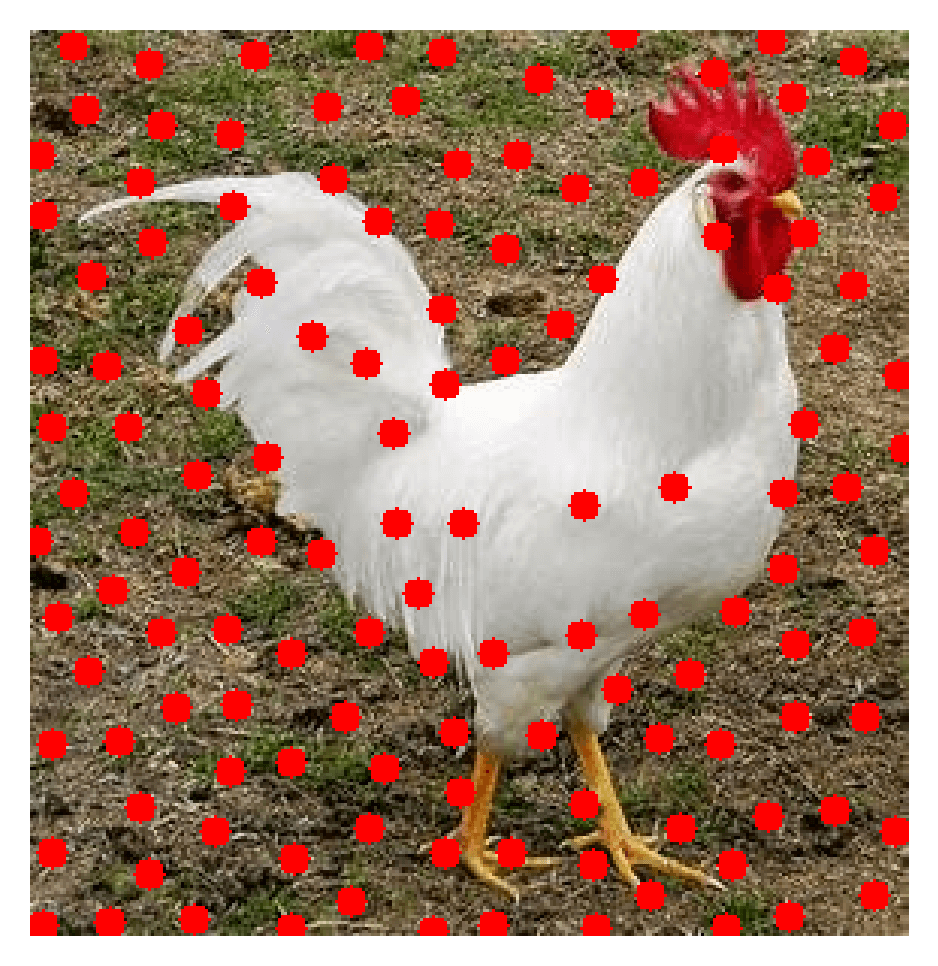
\includegraphics[width=0.9\textwidth]{images/1/1-data_analysis-POI_chicken.png}}
        \captionsetup{width=0.9\linewidth}
        \captionsetup{justification=centering}
        \caption{First chicken in data.}
    \end{subfigure}
    \hspace{1cm}
    \begin{subfigure}{.52\textwidth}
        \centering
        \fbox{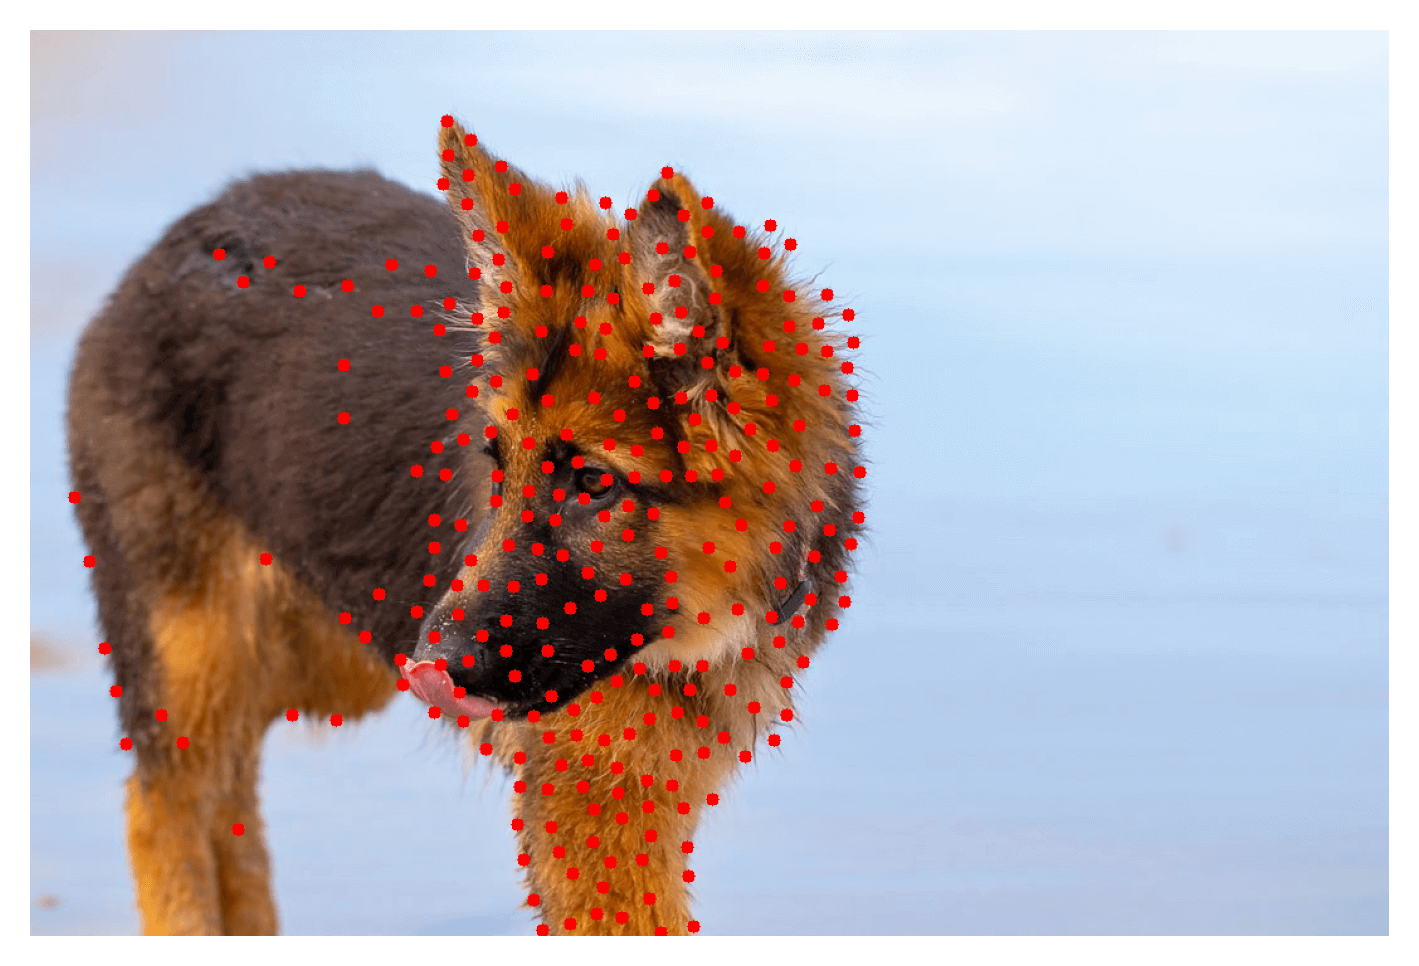
\includegraphics[width=0.9\textwidth]{images/1/1-data_analysis-POI_german_shepherd.png}}
        \captionsetup{width=0.9\linewidth}
        \captionsetup{justification=centering}
        \caption{First German shepherd in train data}
    \end{subfigure}
    \captionsetup{width=0.8\linewidth}
    \captionsetup{justification=centering}
    \caption{Points of interest found by the Shi-Tomasi corner detector.}
    \label{fig:1-poi}
\end{figure*}


%------------------------------------

\section*{The numerical representation}

These interesting points now need to be represented by numerical values that have actual meaning.
Remember from section \ref{section:DA_deeper_look_data} that the provided images differ a lot.
Thus the numerical representation, generated by a descriptor, has to be so that it minifies the impact of different lighting, scaling...
afterwards, these values can be clustered together using the \texttt{createCodebook} function which uses Mini-Batch K-Means clustering.
This could also benefit from fine-tuning.

An overview showing histograms for each word (cluster) and a corresponding correlation matrix when opting for SIFT with 30 clusters is shown in figure \ref{fig:1-cm}.
It is visible that the values are normalized.
This would have to be checked for all descriptors used and perhaps some outliers would need to be removed.
The correlation between these clusters doesn't seem too dramatic in this case ($|$correlation value$| \neq 1 $).
A low correlation between clusters is mostly positive for model building since it suggests each cluster represent a distinct concept.
This is again something that would have to be checked for different parameters.

\begin{figure}[H]
    \centering
    \begin{subfigure}{.45\textwidth}
        \centering
        \fbox{\includegraphics[width=0.7\textwidth]{images/1/1-data_analysis-feature_representation.png}}
        \captionsetup{width=0.9\linewidth}
        \captionsetup{justification=centering}
        \caption{Histogram for each cluster.}
    \end{subfigure}
    \hspace{1cm}
    \begin{subfigure}{.45\textwidth}
        \centering
        \fbox{\includegraphics[width=0.8\textwidth]{images/1/1-data_analysis-correlation_matrix.png}}
        \captionsetup{width=0.9\linewidth}
        \captionsetup{justification=centering}
        \caption{Correlation matrix for all clusters.}
    \end{subfigure}
    \captionsetup{width=0.8\linewidth}
    \captionsetup{justification=centering}
    \caption{Data analysis of encoded images using SIFT with 30 clusters.}
    \label{fig:1-cm}
\end{figure}


%------------------------------------------------------------------------------------------------------------------------------------------------


\chapter*{Appendix B: Important LBM parameters}
\addcontentsline{toc}{chapter}{Appendix B: Important LBM parameters}

As found in the documentation of the \texttt{LogisticRegression} function available in the SciKit Learn library there are multiple (optional) parameters \citep{scikit_learn}.
The most interesting ones are:

\begin{itemize}
    \item \emph{solver}
    \begin{itemize}
        \item Specifies which solver should be used for the optimization problem in the model.
        \item \emph{lbfgs} is used as default and whilst a little slow, this parameter doesn't require further fine-tuning.
    \end{itemize}
    \item \emph{penalty}
    \begin{itemize}
        \item Since the \emph{lbfgs} solver is used, the default \emph{l2} penalization norm is the only one that can be used.
    \end{itemize}
    \item \emph{class\_weight}
    \begin{itemize}
        \item This parameter defaults to None but can be set to balanced to take into account the unbalance in our data, as discussed in section \ref{section:DA_data_distribution}.
        \item The results with this parameter set to balanced will be studied.
    \end{itemize}
    \item \emph{C}
    \begin{itemize}
        \item The regularisation hyperparameter C defaults to 1. Fine-tuning this could boost performance.
    \end{itemize}
    \item \emph{max\_iter}
    \begin{itemize}
        \item This parameter can be changed so that convergence might be found, which is not the case right now.
    \end{itemize}
    \item \emph{fit\_intercept}
    \begin{itemize}
        \item Boolean that specifies if a constant (a.k.a. bias or intercept) should be added to the decision function.
        \item The results with this parameter set to true and false should be checked.
    \end{itemize}
\end{itemize}

%------------------------------------------------------------------------------------------------------------------------------------------------

\end{document}
